\begin{center}
    \section{Homología}
\end{center}
\subsection{Motivación}
\begin{ejercicio}
    % ID: 60
Verificar que $R(S)$ tiene la \textit{propiedad universal de un $R$-módulo libre}; es decir, considerando la inclusión $\iota \colon S \hookrightarrow R(S)$ dada por $\iota(s) = 1s \equiv s$, dado cualquier $R$-módulo $M$ y una función $f \colon S \to M$, existe un único homomorfismo de $R$-módulos $\bar{f} \colon R(S) \to M$ tal que $\bar{f} \circ \iota = f$:
\[
\begin{tikzcd}[row sep=large, column sep=large]
S \arrow[r, "\iota", hook] \arrow[dr, "f"'] & R(S) \arrow[d, "\bar{f}", dashed] \\
& M
\end{tikzcd}
\]
\end{ejercicio}
Sea $M$ una variedad suave y consideremos subvariedades $V_i \subset M$, donde todas son \textit{variedades compactas sin frontera}. Siguiendo la idea de Betti, se consideran sumas formales de la forma
\[
k_1 V_1 + k_2 V_2 + \dots + k_r V_r, \;\; k_i \in \mathbb{Z} \quad (k_i > 0, \; k_i < 0).
\]
\[
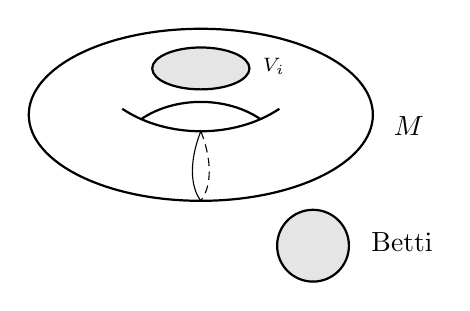
\begin{tikzpicture}[scale=0.95]
    % Variedad ambiente M (toro)
    \draw[thick] (0,0) ellipse (2.3 and 1.15);
    \draw[thick] (-1.05, 0.08) .. controls (-0.45, -0.32) and (0.45, -0.32) .. (1.05, 0.08);
    \draw[thick] (-0.8, -0.06) .. controls (-0.35, 0.25) and (0.35, 0.25) .. (0.8, -0.06);

    % Subvariedad V_i dentro de M
    \fill[gray!20] (0, 0.62) ellipse (0.65 and 0.28);
    \draw[thick] (0, 0.62) ellipse (0.65 and 0.28);
    \node[right] at (0.7, 0.65) {$\scriptstyle V_i$};

    % Curva meridiana inferior
    \draw[thin] (0, -0.22) .. controls (-0.15, -0.6) and (-0.15, -0.95) .. (0, -1.15);
    \draw[thin, densely dashed] (0, -0.22) .. controls (0.15, -0.6) and (0.15, -0.95) .. (0, -1.15);

    \node[right] at (2.45, -0.15) {$M$};

    % Disco / subvariedad aparte (Betti)
    \begin{scope}[shift={(1.5, -1.75)}]
        \fill[gray!20] (0,0) circle (0.48);
        \draw[thick] (0,0) circle (0.48);
        \node[right] at (0.65, 0.05) {Betti};
    \end{scope}
\end{tikzpicture}
\]

Sea ahora $K$ un complejo simplicial y consideremos un $q$-simplejo $s = \{v_0, v_1, \dots, v_q\}$. La \textit{frontera} de $s$ consiste en sus $(q-1)$-caras, es decir, la suma formal
\[
\{\hat{v}_0, v_1, \dots, v_q\} + \{v_0, \hat{v}_1, \dots, v_q\} + \dots + \{v_0, v_1, \dots, v_{q-1}, \hat{v}_q\},
\]
donde $\hat{v}_i$ indica que el vértice $v_i$ se omite. Por ejemplo, para un $2$-simplejo $s = \{v_0, v_1, v_2\}$ tenemos:
\begin{equation}
\label{diag:2_simplejo}
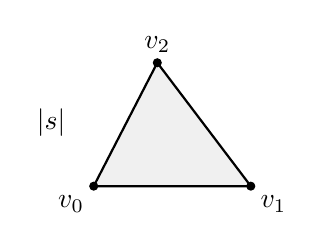
\begin{tikzpicture}[baseline=(current bounding box.center), scale=0.95]
    \coordinate (V0) at (0, 0);
    \coordinate (V1) at (2.1, 0);
    \coordinate (V2) at (0.85, 1.65);

    \fill[gray!12] (V0) -- (V1) -- (V2) -- cycle;
    \draw[thick] (V0) -- (V1) -- (V2) -- cycle;

    \filldraw (V0) circle (1.5pt) node[below left] {$v_0$};
    \filldraw (V1) circle (1.5pt) node[below right] {$v_1$};
    \filldraw (V2) circle (1.5pt) node[above] {$v_2$};

    \node[left] at (-0.25, 0.85) {$|s|$};
\end{tikzpicture}
\qquad \qquad
\{v_1, v_2\} + \{v_0, v_2\} + \{v_0, v_1\}.
\end{equation}

\begin{definicion}
Denotamos por $K_q$ al conjunto de los $q$-simplejos de $K$ y consideramos el $\mathbb{Z}_2$-módulo libre $\mathbb{Z}_2(K_q)$, cuyos elementos son de la forma
\[
\sum_{s \in K_q} r_s s, \;\; r_s \in \mathbb{Z}_2.
\]
\end{definicion}
\begin{definicion}
Definimos el \textit{operador frontera} $\partial_q \colon \mathbb{Z}_2(K_q) \to \mathbb{Z}_2(K_{q-1})$ mediante
\[
\partial_q\big(\{v_0, v_1, \dots, v_q\}\big) = \sum_{i=0}^q \{v_0, v_1, \dots, \hat{v}_i, \dots, v_q\},
\]
donde $\hat{v}_i$ indica que se omite el vértice $v_i$.
\end{definicion}

%%%% Clase 30 del 19/10/26 inciada el 18/11/26 terminada el 18/11/2026

%%%% Clase 31 del 21/10/26 inciada el 17/11/26

\begin{ejemplo}
Consideremos el $2$-simplejo $\{v_0, v_1, v_2\}$ \ref{diag:2_simplejo}.
Calculando los operadores frontera con coeficientes en $\mathbb{Z}_2$, tenemos:
\begin{align*}
\partial_2\big(\{v_0, v_1, v_2\}\big) &= \{v_1, v_2\} + \{v_0, v_2\} + \{v_0, v_1\}, \\[1ex]
\partial_1 \partial_2\big(\{v_0, v_1, v_2\}\big) &= \partial_1\big(\{v_1, v_2\}\big) + \partial_1\big(\{v_0, v_2\}\big) + \partial_1\big(\{v_0, v_1\}\big) \\
&= v_1 + v_2 + v_0 + v_2 + v_0 + v_1 = 0.
\end{align*}
\end{ejemplo}

\begin{ejercicio}
    % ID: 61
Verificar que ${\partial_{q-1} \circ \partial_q = 0}$.
\end{ejercicio}
\begin{ejemplo}
Consideremos $S^2$ y la triangulación $S^2 \cong |Q|$, donde $V_Q = \{v_0, v_1, v_2, v_3\}$:
\[
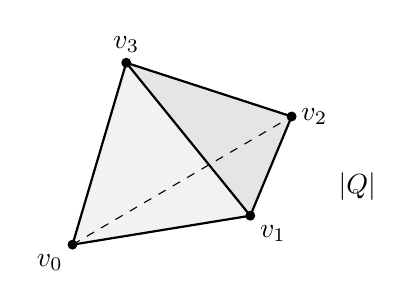
\begin{tikzpicture}[baseline=(current bounding box.center), scale=1.05]
    \coordinate (V0) at (0, 0);
    \coordinate (V1) at (2.15, 0.35);
    \coordinate (V2) at (2.65, 1.55);
    \coordinate (V3) at (0.65, 2.2);

    % Caras frontales con sombreado suave
    \fill[gray!10] (V0) -- (V1) -- (V3) -- cycle;
    \fill[gray!20] (V1) -- (V2) -- (V3) -- cycle;

    % Arista oculta
    \draw[dashed, thin] (V0) -- (V2);

    % Aristas visibles
    \draw[thick] (V0) -- (V1) -- (V2) -- (V3) -- cycle;
    \draw[thick] (V1) -- (V3);

    % Vértices y etiquetas
    \filldraw (V0) circle (1.5pt) node[below left] {$v_0$};
    \filldraw (V1) circle (1.5pt) node[below right] {$v_1$};
    \filldraw (V2) circle (1.5pt) node[right] {$v_2$};
    \filldraw (V3) circle (1.5pt) node[above] {$v_3$};

    \node[right] at (3.1, 0.7) {$|Q|$};
\end{tikzpicture}
\]
Tomamos la cadena $C(Q)$ formada por los simplejos de dimensión $2$:
\[
C(Q) = \{v_0, v_1, v_3\} + \{v_1, v_2, v_3\} + \{v_0, v_1, v_2\} + \{v_0, v_2, v_3\}.
\]
Al aplicar el operador frontera $\partial_2$, cada $1$-simplejo aparece exactamente dos veces, por lo que se cancelan en $\mathbb{Z}_2$:
\begin{align*}
\partial_2 C(Q) &= \overset{1}{\{v_1, v_3\}} + \overset{2}{\{v_0, v_3\}} + \overset{3}{\{v_0, v_1\}} + \overset{4}{\{v_2, v_3\}} + \overset{1}{\{v_1, v_3\}} + \overset{5}{\{v_1, v_2\}} \\[0.5ex]
&\phantom{=} + \underset{5}{\{v_1, v_2\}} + \underset{6}{\{v_0, v_2\}} + \underset{3}{\{v_0, v_1\}} + \underset{4}{\{v_2, v_3\}} + \underset{2}{\{v_0, v_3\}} + \underset{6}{\{v_0, v_2\}} = 0.
\end{align*}
\end{ejemplo}

\begin{nota}
Sea $M^n$ una \textit{variedad suave}, \textit{compacta}, \textit{conexa} y \textit{sin frontera}. Sea $Q$ una triangulación de $M$, es decir, $|Q| \xrightarrow[\;\cong\;]{\;h\;} M^n$. Entonces $Q$ satisface:
\begin{enumerate}
    \item Todo simplejo de $Q$ es cara de un $n$-simplejo.
    \item Dado $s$ un $(n-1)$-simplejo de $Q$, entonces $s$ es cara de \textit{exactamente dos} $n$-simplejos de $Q$.
\end{enumerate}
\end{nota}
\begin{prop}
Sea $Q$ una triangulación de una variedad $M^n$ suave, compacta, conexa y sin frontera. Entonces la cadena
\[
C(Q) = \sum_{s \in Q_n} s \in \mathbb{Z}_2(Q)
\]
satisface $\partial_n\big(C(Q)\big) = 0$.
\end{prop}

\begin{dem}
Aplicando el operador frontera, tenemos que
\[
\partial_n\big(C(Q)\big) = \partial_n\Big( \sum_{s \in Q_n} s \Big) = \sum_{s \in Q_n} \partial_n(s).
\]
Los elementos de esta cadena son los $(n-1)$-simplejos de $Q$ y cada uno aparece exactamente dos veces, pues cada $(n-1)$-simplejo es cara de exactamente dos $n$-simplejos por la Nota anterior. Como cada elemento tiene orden $2$, se obtiene que
\[
\sum_{s \in Q_n} \partial_n(s) = 0, \; \text{es decir,} \; C(Q) \in \ker \partial_n.
\]
\end{dem}

\begin{definicion}
A los elementos de $\ker \partial_n$ se les llama \textit{$n$-ciclos}, y a cada variedad de dimensión $n$ suave, compacta, conexa y sin frontera le asociamos el \textit{$n$-ciclo} $C(Q)$.
\end{definicion}

\begin{definicion}
Sea $K$ un complejo simplicial y consideremos la familia de $\mathbb{Z}_2$-módulos y homomorfismos
\[
\cdots \longrightarrow \mathbb{Z}_2(K_{q+1}) \xrightarrow{\;\partial_{q+1}\;} \mathbb{Z}_2(K_q) \xrightarrow{\;\partial_q\;} \mathbb{Z}_2(K_{q-1}) \longrightarrow \cdots \xrightarrow{\;\partial_1\;} \mathbb{Z}_2(K_0).
\]
Por el ejercicio anterior, $\partial_q \circ \partial_{q+1} = 0$; por lo tanto, $\operatorname{Im} \partial_{q+1} \subset \ker \partial_q$. A esta familia se le llama un \textit{complejo de cadenas de $\mathbb{Z}_2$-módulos}. Definimos
\[
H_q(K; \mathbb{Z}_2) = \raisebox{0.2ex}{$\ker \partial_q$} \big/ \raisebox{-0.2ex}{$\operatorname{Im} \partial_{q+1}$}
\]
como la \textit{$q$-homología simplicial con coeficientes en $\mathbb{Z}_2$} de $K$.
\end{definicion}

\begin{nota}
Notemos que si este módulo es $0$, lo que nos dice es que cualquier $q$-ciclo es \textit{frontera} de una $(q+1)$-cadena. Si el módulo es distinto de $0$, hay un $q$-ciclo que no es frontera.

En particular, si $M^n$ es una variedad suave como antes y $|Q| \cong M$, entonces $[C(Q)] \in H_n(Q; \mathbb{Z}_2)$. Se puede probar que $[C(Q)] \neq 0$ y es el generador de $H_n(Q; \mathbb{Z}_2) \cong \mathbb{Z}_2$.
\end{nota}

\begin{definicion}
Un \textit{complejo simplicial ordenado} es un complejo simplicial $K$ junto con un orden parcial $<$ en sus vértices, de manera que cada simplejo de $K$ está totalmente ordenado. Esto se puede hacer dando un orden total a los vértices o considerando la \textit{subdivisión baricéntrica} de $K$.
\end{definicion}

\begin{definicion}
Sea $K$ un complejo simplicial. La \textit{subdivisión baricéntrica} de $K$, denotada por $\operatorname{sd} K$, es el complejo simplicial dado por $V_{\operatorname{sd} K} = K$, que está parcialmente ordenado por la inclusión de los simplejos. Un $q$-simplejo de $\operatorname{sd} K$ es de la forma
\[
\{ s_0 \subsetneq s_1 \subsetneq \dots \subsetneq s_q \},
\]
donde los $s_i$ son simplejos de $K$.
\end{definicion}

\begin{ejemplo}
En la subdivisión baricéntrica de un $2$-simplejo $\{v_0, v_1, v_2\}$, el $2$-simplejo sombreado corresponde a la cadena de inclusiones indicada:
\[
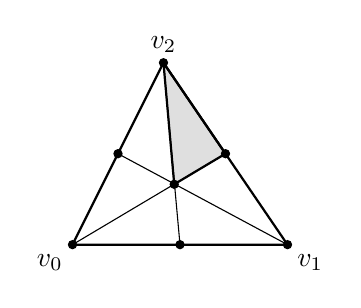
\begin{tikzpicture}[baseline=(current bounding box.center), scale=1.05]
    % Vértices principales
    \coordinate (V0) at (0, 0);
    \coordinate (V1) at (2.6, 0);
    \coordinate (V2) at (1.1, 2.2);

    % Baricentros de las 1-caras (puntos medios)
    \coordinate (M01) at (1.3, 0);
    \coordinate (M12) at (1.85, 1.1);
    \coordinate (M02) at (0.55, 1.1);

    % Baricentro del 2-simplejo
    \coordinate (B) at (1.23, 0.73);

    % Sombreado del 2-simplejo {{v_2} \subsetneq {v_2, v_1} \subsetneq {v_0, v_1, v_2}}
    \fill[gray!25] (V2) -- (M12) -- (B) -- cycle;

    % Líneas de la subdivisión baricéntrica
    \draw[thin] (V0) -- (M12);
    \draw[thin] (V1) -- (M02);
    \draw[thin] (V2) -- (M01);

    % Aristas del 2-simplejo sombreado resaltadas
    \draw[thick] (V2) -- (M12) -- (B) -- cycle;

    % Contorno exterior del 2-simplejo original
    \draw[thick] (V0) -- (V1) -- (V2) -- cycle;

    % Vértices de sd K
    \foreach \p in {V0, V1, V2, M01, M12, M02, B} {
        \filldraw (\p) circle (1.4pt);
    }

    % Etiquetas
    \node[below left] at (V0) {$v_0$};
    \node[below right] at (V1) {$v_1$};
    \node[above] at (V2) {$v_2$};
\end{tikzpicture}
\; \; \;
\big\{ \{v_2\} \subsetneq \{v_2, v_1\} \subsetneq \{v_0, v_1, v_2\} \big\} \in \operatorname{sd} K.
\]
\end{ejemplo}

\begin{nota}
Se tiene que $|\operatorname{sd} K| \cong |K|$.
\end{nota}
\begin{definicion}
Sea $K$ un complejo simplicial ordenado. Definimos el $R$-módulo
\[
C_q^<(K; R) = R\Big( \big\{ (v_0, v_1, \dots, v_q) \;\big|\; \{v_0, v_1, \dots, v_q\} \in K_q \; \text{y} \; v_0 < v_1 < \dots < v_q \big\} \Big),
\]
donde la base son los $q$-simplejos de $K$, con \textit{operador frontera} $\partial_q^< \colon C_q^<(K; R) \to C_{q-1}^<(K; R)$ dado por
\[
\partial_q^<(v_0, v_1, \dots, v_q) = \sum_{i=0}^q (-1)^i (v_0, v_1, \dots, \hat{v}_i, \dots, v_q).
\]
\end{definicion}

\begin{ejercicio}
    % ID: 62
Verificar que $\partial_q^< \circ \partial_{q+1}^< = 0$; por lo tanto, $\operatorname{Im} \partial_{q+1}^< \subset \ker \partial_q^<$.
\end{ejercicio}

\begin{definicion}
Definimos el \textit{$R$-módulo de homología} de $K$ como
\[
H_q(K; R) = \raisebox{0.2ex}{$\ker \partial_q^<$} \Big/ \raisebox{-0.2ex}{$\operatorname{Im} \partial_{q+1}^<$}.
\]
\end{definicion}

\begin{ejercicio}
    % ID: 63
Sean $V_K = \{v_0, v_1, v_2\}$ y
\[
K = \big\{ \{v_0\}, \{v_1\}, \{v_2\}, \{v_0, v_1\}, \{v_1, v_2\}, \{v_0, v_2\} \big\},
\]
de modo que $|K| \cong S^1$. Verificar que
\[
H_q(K; R) \cong 
\begin{cases}
    R, & \text{si } q = 0 \; \text{o} \; 1, \\
    0, & \text{si } q \neq 0, 1.
\end{cases}
\]
\end{ejercicio}

\subsection{Complejos de cadena de $R$-módulos}

%%%% Clase 31 del 21/10/26 inciada el 18/11/26 terminada el 18/11/2026

%%%%%% Clase ????(32) del 23/10/2026 iniciada el 23/10/2026
\begin{definicion}
A una familia de $R$-módulos $C_* = \{C_q\}_{q \in \mathbb{Z}}$ y homomorfismos $\partial_q \colon C_q \to C_{q-1}$ tales que $\partial_q \circ \partial_{q+1} = 0$ se le llama \textit{complejo de cadenas de $R$-módulos}, y su \textit{homología} se define como
\[
H_q(C_*; R) = \raisebox{0.2ex}{$\ker \partial_q$} \big/ \raisebox{-0.2ex}{$\operatorname{Im} \partial_{q+1}$}.
\]
\end{definicion}
\begin{definicion}
Un \textit{morfismo de cadenas} $\psi \colon C_* \to C'_*$ es una colección de homomorfismos de $R$-módulos $\psi_q \colon C_q \to C'_q$ tales que conmuta el siguiente diagrama para cada $q$:
\[
\begin{tikzcd}[row sep=large, column sep=large]
C_q \arrow[r, "\partial_q"] \arrow[d, "\psi_q"'] & C_{q-1} \arrow[d, "\psi_{q-1}"] \\
C'_q \arrow[r, "\partial'_q"'] & C'_{q-1}
\end{tikzcd}
\]
\end{definicion}
\begin{definicion}
    Dado un morfismo de cadena $\psi:(C_*,\partial_*)\to(C_*',\partial_*')$. Definimos el homomorfismo
    \begin{equation*}
        \psi_*:H_q(C_*,\partial_*)\to H_q(C_*,\partial_*')
    \end{equation*}
    tal que $\psi_*[z]=[\psi(z)]$. Donde $[z]$ es la cadena de homología de $q$-ciclos $z\in Z_q=\ker\partial_q$ y los $q$-frontera $B_q=\im\partial_{q+1}.$
\end{definicion}
\begin{ejercicio}
    % ID: 64
    Ver que $\psi_*$ está bien definida.
\end{ejercicio}
\begin{ejemplo}
Un ejemplo importante de complejo de cadenas lo proporcionan los complejos ordenados. Dado un morfismo simplicial entre complejos ordenados $f \colon K^< \to L^<$, deseamos definir un morfismo de cadenas
\[
f_\# \colon C_q^<(K; R) \longrightarrow C_q^<(L; R).
\]
Si intentamos definirlo en los generadores básicos como
\[
f_\#\big((v_0, v_1, \dots, v_q)\big) = \big(f(v_0), f(v_1), \dots, f(v_q)\big) \quad \text{con } v_0 < v_1 < \dots < v_q,
\]
el problema que surge es que si $f$ no es inyectiva, la tupla resultante puede tener vértices repetidos y, por lo tanto, **no sería un $q$-simplejo de $L$**. En este caso, definimos
\[
f_\#((v_0, v_1, \dots, v_q)) = 0.
\]
\end{ejemplo}
\begin{ejemplo}
Un ejemplo importante de complejo de cadenas lo proporcionan los complejos ordenados. Dado un morfismo simplicial entre complejos ordenados $f \colon K^< \to L^<$, deseamos definir un morfismo de cadenas
\[
f_\# \colon C_q^<(K; R) \longrightarrow C_q^<(L; R).
\]
Si intentamos definirlo en los generadores básicos como
\[
f_\#(v_0, v_1, \dots, v_q) = (f(v_0), f(v_1), \dots, f(v_q)) \; \text{con } v_0 < v_1 < \dots < v_q,
\]
el problema que surge es que si $f$ no es inyectiva, la tupla resultante tiene vértices repetidos y no es un $q$-simplejo de $L$; en este caso, definimos $f_\#(v_0, v_1, \dots, v_q) = 0$. 

Por el contrario, si $f$ es inyectiva en los vértices, hay que escribir los vértices $f(v_i)$ en el orden $<'$ de $L$ y agregar un signo, definiendo:
\[
f_\#(v_0, v_1, \dots, v_q) = (-1)^{\operatorname{sgn}(\sigma)} (f(v_{i_0}), f(v_{i_1}), \dots, f(v_{i_q})),
\]
donde $\sigma$ es la permutación que transforma el orden original en el orden creciente $<'$ de $L$.
\end{ejemplo}
\begin{definicion}
Sea $K$ un complejo simplicial. Definimos el \textit{complejo de cadenas secuencial} de $K$, que denotamos por $\mathcal{C}_*(K; R)$, dado en cada grado $q$ por
\[
\mathcal{C}_q(K; R) = R(\{ (v_0, v_1, \dots, v_q) \mid \{v_0, v_1, \dots, v_q\} \in K \}),
\]
con operador frontera $\partial_q \colon \mathcal{C}_q(K; R) \to \mathcal{C}_{q-1}(K; R)$ definido mediante
\[
\partial_q(v_0, v_1, \dots, v_q) = \sum_{i=0}^q (-1)^i (v_0, v_1, \dots, \hat{v}_i, \dots, v_q).
\]
Este operador está bien definido, pues si $\{v_0, v_1, \dots, v_q\} \in K$, entonces $\{v_0, v_1, \dots, \hat{v}_i, \dots, v_q\} \in K$.
\end{definicion}

\begin{nota}
Se puede probar que
\[
H_q(\mathcal{C}_*(K; R), \partial_*) \cong H_q(C_*^<(K; R), \partial_*^<).
\]
\end{nota}
\begin{definicion}
    Sea $f:K\to L$ un morfismo simplicial. Definimos 
    \begin{align*}
        f_{\#}:\mathscr{C}_*(K,R)&\to\mathscr{C}_*(L,R)\\
        (v_0,\ldots,v_q)&\mapsto (f(v_1),\ldots,f(v_q))
    \end{align*}
\end{definicion}
\begin{ejercicio}
    % ID: 65
    Ver que $f_\#$ es un morfismo de cadena y, por lo tanto, define un homomorfismo en homología.
\end{ejercicio}

Se tiene la conjetura (Hauptvermutung): sea $K$ y $Q$ complejos simpliciales tales que $|K|\cong |Q|$, entonces existen \textit{subdivisiones} $K'$ y $Q'$ tales que $K'\cong Q'$. Esta conjetura es falsa (Milnor, 1961).

\begin{teorema}[S.W.Alexander, 1915]
Sea $K$ y $L$ complejos simpliciales tales que $|K|\cong |L|$, entonces $H_q(K,R)\cong H_q(L,R)$ %%%completar
\end{teorema}
\begin{coro}
Sea $X$ un espacio triangulable; entonces los módulos de homología simplicial son independientes, módulo isomorfismo, de la triangulación.
\end{coro}

\begin{dem}
Si tenemos dos triangulaciones
\[
|K| \xrightarrow[\;\cong\;]{\;f\;} X \xleftarrow[\;\cong\;]{\;g\;} |Q|,
\]
entonces $g^{-1} \circ f \colon |K| \xrightarrow{\;\cong\;} |Q|$ es un homeomorfismo. Por lo tanto,
\[
H_q(K; R) \cong H_q(Q; R).
\]
\end{dem}
\begin{nota}
Existe también un complejo de cadenas \textit{orientado} $(C_*(K; R), \partial_*)$. Dando un orden a $K$, se puede ver que la aplicación
\[
C_q^<(K; R) \xrightarrow[\;\cong\;]{\;\beta_q\;} C_q(K; R),
\]
definida como
\[
\beta_q(v_0, v_1, \dots, v_q) = [v_0, v_1, \dots, v_q], \; v_0 < v_1 < \dots < v_q,
\]
donde $[v_0, v_1, \dots, v_q]$ denota la \textit{clase de orientación} de un simplejo $s = \{v_0, v_1, \dots, v_q\}$, es un isomorfismo. El operador frontera está dado por
\[
\partial_q[v_0, v_1, \dots, v_q] = \sum_{i=0}^q (-1)^i [v_0, v_1, \dots, \hat{v}_i, \dots, v_q].
\]
\end{nota}
\begin{definicion}
Para cada $q \geq 0$, definimos el homomorfismo de $R$-módulos
\[
\varphi_q \colon C_q^<(K; R) \longrightarrow R(\operatorname{Map}(\Delta^q, |K|))
\]
sobre los generadores básicos $(v_0, v_1, \dots, v_q)$ (con $v_0 < v_1 < \dots < v_q$) mediante
\[
\varphi_q(v_0, v_1, \dots, v_q) = \sigma_{(v_0, v_1, \dots, v_q)} \in \operatorname{Map}(\Delta^q, |K|) \subset R(\operatorname{Map}(\Delta^q, |K|)),
\]
y extendiéndolo por linealidad. Se busca definir un operador frontera $\partial'_q$ que haga conmutar el siguiente diagrama:
\[
\begin{tikzcd}[row sep=large, column sep=large]
C_q^<(K; R) \arrow[r, "\varphi_q"] \arrow[d, "\partial_q^<"'] & \operatorname{Map}(\Delta^q, |K|) \arrow[r, phantom, "\subset"] &[-3.2em] R(\operatorname{Map}(\Delta^q, |K|)) \arrow[d, "\partial'_q", dashed] \\
C_{q-1}^<(K; R) \arrow[r, "\varphi_{q-1}"'] & \operatorname{Map}(\Delta^{q-1}, |K|) \arrow[r, phantom, "\subset"] & R(\operatorname{Map}(\Delta^{q-1}, |K|))
\end{tikzcd}
\]
donde el operador frontera $\partial_q^<$ está dado por
\[
\partial_q^<(v_0, v_1, \dots, v_q) = \sum_{i=0}^q (-1)^i (v_0, v_1, \dots, \hat{v}_i, \dots, v_q).
\]
\end{definicion}
\begin{definicion}
Para cada $0 \leq i \leq q$, definimos la \textit{inclusión de cara} $F_q^i \colon \Delta^{q-1} \hookrightarrow \Delta^q$ dada por
\[
F_q^i(t_0, \dots, t_{q-1}) = (t_0, \dots, t_{i-1}, 0, t_i, \dots, t_{q-1}),
\]
o bien, sobre los vértices de la base canónica, por
\[
F_q^i(e_j) =
\begin{cases}
    e_j, & \text{si } j < i, \\
    e_{j+1}, & \text{si } j \geq i.
\end{cases}
\]
\[
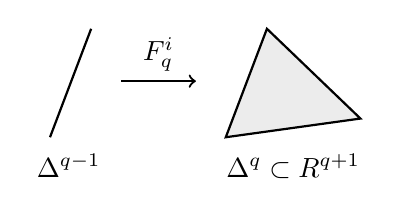
\begin{tikzpicture}[baseline=(current bounding box.center), scale=0.95]
    % Simplejo \Delta^{q-1}
    \draw[thick] (0, 0) -- (0.55, 1.45);
    \node[below] at (0.25, -0.1) {$\Delta^{q-1}$};

    % Flecha F_q^i
    \draw[->, thick] (0.95, 0.75) -- (1.95, 0.75) node[midway, above] {$F_q^i$};

    % Simplejo \Delta^q
    \coordinate (A) at (2.35, 0);
    \coordinate (B) at (4.15, 0.25);
    \coordinate (C) at (2.9, 1.45);

    \fill[gray!15] (A) -- (B) -- (C) -- cycle;
    \draw[thick] (A) -- (B) -- (C) -- cycle;
    \node[below] at (3.25, -0.1) {$\Delta^q \subset \mathbb{R}^{q+1}$};
\end{tikzpicture}
\]
\end{definicion}

\begin{lema}
Para cada $0 \leq i \leq q$, se cumple que
\[
\sigma_{(v_0, v_1, \dots, \hat{v}_i, \dots, v_q)} = \sigma_{(v_0, v_1, \dots, v_q)} \circ F_q^i.
\]
\end{lema}

\begin{dem}
Para todo $(t_0, t_1, \dots, t_{q-1}) \in \Delta^{q-1}$, tenemos que
\begin{align*}
(\sigma_{(v_0, v_1, \dots, v_q)} \circ F_q^i)(t_0, t_1, \dots, t_{q-1}) &= \sigma_{(v_0, v_1, \dots, v_q)}(t_0, \dots, t_{i-1}, 0, t_i, \dots, t_{q-1}) \\
&= t_0 v_0 + \dots + t_{i-1} v_{i-1} + t_i v_{i+1} + \dots + t_{q-1} v_q \\
&= \sigma_{(v_0, v_1, \dots, \hat{v}_i, \dots, v_q)}(t_0, t_1, \dots, t_{q-1}).
\end{align*}
\end{dem} 

\begin{definicion}
Denotamos $R(\operatorname{Map}(\Delta^q, |K|)) \equiv S_q(|K|)$. Sea $\sigma \colon \Delta^q \to |K|$ una función continua; definimos el operador frontera $\partial'_q \colon S_q(|K|) \to S_{q-1}(|K|)$ sobre los generadores mediante
\[
\partial'_q(\sigma) = \sum_{i=0}^q (-1)^i \sigma \circ F_q^i,
\]
\end{definicion}

\begin{prop}
$\varphi$ es un morfismo de cadenas; es decir, para cada $q$ conmuta el siguiente diagrama:
\[
\begin{tikzcd}[row sep=large, column sep=large]
C_q^<(K; R) \arrow[r, "\partial_q^<"] \arrow[d, "\varphi_q"'] & C_{q-1}^<(K; R) \arrow[d, "\varphi_{q-1}"] \\
S_q(|K|) \arrow[r, "\partial'_q"'] & S_{q-1}(|K|)
\end{tikzcd}
\]
\end{prop}
%%%% Clase 32 del 23/10/26 inciada el 23/10/26 terminada el 18/11/2026

%%%%%% Clase 33 del 26/10/2026 iniciada el 18/11/2026
\begin{dem}
Para verificar que el diagrama anterior conmuta, basta comprobar la igualdad sobre los generadores básicos $(v_0, v_1, \dots, v_q)$ de $C_q^<(K; R)$. Por un lado, se tiene que
\[
\partial'_q \varphi_q(v_0, v_1, \dots, v_q) = \partial'_q(\sigma_{(v_0, \dots, v_q)}) = \sum_{i=0}^q (-1)^i \sigma_{(v_0, \dots, v_q)} \circ F_q^i.
\]
Por otro lado, aplicando $\varphi_{q-1} \circ \partial_q^<$ y utilizando el lema anterior, obtenemos
\begin{align*}
\varphi_{q-1} \partial_q^<(v_0, v_1, \dots, v_q) &= \varphi_{q-1}\left( \sum_{i=0}^q (-1)^i (v_0, \dots, \hat{v}_i, \dots, v_q) \right) \\
&= \sum_{i=0}^q (-1)^i \sigma_{(v_0, \dots, \hat{v}_i, \dots, v_q)} \\
&{=} \sum_{i=0}^q (-1)^i \sigma_{(v_0, \dots, v_q)} \circ F_q^i.
\end{align*}
Por lo tanto, $\partial'_q \circ \varphi_q = \varphi_{q-1} \circ \partial_q^<$, y por linealidad $\varphi$ es un morfismo de cadenas.
\end{dem}

\begin{definicion}
La fórmula para $\partial'_q$ tiene sentido para cualquier espacio topológico $X$ y cualquier función continua $\sigma \colon \Delta^q \to X$. Definimos el $R$-módulo de \textit{$q$-cadenas singulares} (introducidas por Lefschetz) como
\[
S_q(X) \equiv R(\operatorname{Map}(\Delta^q, X)),
\]
con \textit{operador frontera} $\partial_q \colon S_q(X) \to S_{q-1}(X)$ dado sobre los generadores por
\[
\partial_q(\sigma) = \sum_{i=0}^q (-1)^i \sigma \circ F_q^i,
\]
\end{definicion}
 \begin{nota}
     A los elementos de $S_q(X)$ se le llama cadenas singulares con coeficientes en $R$.
 \end{nota}
 \begin{ejercicio}
    % ID: 66
     $F_q^i\circ F_{q-1}^i=F_q^j\circ F_{q-1}^{i-1}$ para todo $j<i$.
 \end{ejercicio}
 \begin{ejercicio}
    % ID: 67
 Ver que $\partial_q:S_q\to S_{q-1}$ satisface que $\partial_q\circ \partial_{q+1}=0$.
 \end{ejercicio}
 \begin{definicion}
     Definimos el $q$-módulo de homología singular de $X$ con coeficientes en $R$ como $H_q(X,R)=\ker \partial_q/\im\partial_{q-1}$. Además, $\ker\partial_q=Z_q(X)$ son los $q$-cíclos y $\im\partial_{q}$ %%%%% acompletar
 \end{definicion}

%%%%% FALTA

\begin{lema}
    $f_\#$ es un morfismo de cadena.
\end{lema} 
\begin{dem}
    Consideremos el siguiente diagrama
    \begin{equation*}
        \begin{tikzcd}[row sep=large, column sep=large]
            S_q(X)\arrow[r,"\partial_q^X"]\arrow[d,"f_\#"] & S_{q-1}(Y\arrow[d,"f_\#"]\\
            S_q(X)\arrow[r,"\partial_q^Y"] & S_{q-1}(Y)
        \end{tikzcd}
    \end{equation*}
    Sea $\sigma\in S_q(X)$. Entonces
    \begin{align*}
        \partial_q^Yf_\#(\sigma)&= \partial_q^Y(f\circ\sigma)\\
        &=\sum_{i=0}^q(-1)^i(f\circ \sigma)\circ F_q^i.
    \end{align*}
    Por otro lado, 
    \begin{align*}
        f_{\#}\partial_q^X(\sigma)&=f_\#\Big(\sum_{i=0}^q(-1)^i\sigma\circ F^i_q\Big)\\
        &=\sum_{i=0}^q(-1)^i(f\circ \sigma)\circ F_q^i\\
        &=\partial_q^Yf_\#(\sigma).
    \end{align*}
    Por un ejercicio anterior %% agregar eiqueta de ejercicio 
    $f_\#$ pasa a la homología y define $f_*:H_q(X,R)\to H_q(Y,R)$ dado por $f_*[z]=[f_\#(z)]$. Se sigue que la homología singular es un funtor $H_q:\Top\to \Mod$.
    %%%%%% acompletar H_q: Top-> R-mod
\end{dem}
\begin{coro}
    La homología singular es un invariante toplógico.
\end{coro}

\begin{teorema}
    $\varphi:C_*^<(K,R)\to S_q(|K|)$ es un morfismo de cadenas que induce un isomorfismo al pasar a la homología, i.e., existe un isomorfismo
    \begin{equation*}
        \varphi_*:H_q(K,R)\to H_q(|K|,R).
    \end{equation*}
    %%%% Creo es necesario detallar.
\end{teorema} 
\begin{coro}
    $H_*(K,R)$ es un invariante topológico.
\end{coro}
\begin{dem}
     Supongamos $|K|\cong_f |L|$, entonces 
     \begin{align*}
         H_q(K,R)&\equiv H_q(C_*^<(K,R))\\&
         \cong_{\varphi_*}H_q(|K|,R)\\
         &\cong_{f_*}H_q(|L|,R)\\
         &\cong_{\varphi_*}H_q(C_*^<(K,R))\\
         &\equiv H_q(L,R).
     \end{align*}
\end{dem}
\begin{coro}
    Sea $X$ un espacio triangulable, i.e., $|K|\cong_h X$, donde $\dim K=n$. Entonces $H_q(X,R)\cong 0$, siempre que $q>n$.
\end{coro}
\begin{dem}
    Tomemos $C_q^<(K,R)=0$ si $q>n$, por lo tanto,
    \begin{equation*}
        0\cong H_q(K,R)\cong_{\varphi_*} H_(|K|,R)\cong H_q(X,R).
    \end{equation*}
\end{dem}
\begin{prop}
    \begin{equation*}
        H_q(\{x\}.R)=\begin{cases}
            R, & \text{ si } q=0;\\
            0, & \text{ si } q>0. 
        \end{cases}
    \end{equation*}
\end{prop}
\begin{dem}
Consideremos el complejo de cadenas singulares de $\{x\}$:
\[
\begin{tikzcd}[column sep=1.7em, row sep=1.2em]
\cdots \arrow[r] & S_q(\{x\}) \arrow[r, "\partial_q"] \arrow[d, phantom, "\cong"{description, sloped, inner sep=1pt}] & S_{q-1}(\{x\}) \arrow[r] \arrow[d, phantom, "\cong"{description, sloped, inner sep=1pt}] & \cdots \arrow[r] & S_1(\{x\}) \arrow[r, "\partial_1"] \arrow[d, phantom, "\cong"{description, sloped, inner sep=1pt}] & S_0(\{x\}) \arrow[r] \arrow[d, phantom, "\cong"{description, sloped, inner sep=1pt}] & 0 \\
& R(\sigma_q) & R(\sigma_{q-1}) & & R(\sigma_1) & R(\sigma_0) &
\end{tikzcd}
\]
donde $\sigma_q \colon \Delta^q \to \{x\}$ es el único $q$-simplejo singular constante. Como para cada $0 \leq i \leq q$ conmuta el diagrama
\[
\begin{tikzcd}[column sep=2em, row sep=1.8em]
\Delta^{q-1} \arrow[r, "F_q^i"] \arrow[dr, "\sigma_{q-1}"'] & \Delta^q \arrow[d, "\sigma_q"] \\
& \{x\}
\end{tikzcd}
\]
se tiene $\sigma_q \circ F_q^i = \sigma_{q-1}$, por lo que el operador frontera satisface
\[
\partial_q(\sigma_q) = \sum_{i=0}^q (-1)^i \sigma_q \circ F_q^i = \sum_{i=0}^q (-1)^i \sigma_{q-1} =
\begin{cases}
    \sigma_{q-1}, & \text{si } q > 0 \text{ es par}, \\
    0, & \text{si } q \text{ es impar}.
\end{cases}
\]
De aquí se sigue que los módulos de ciclos y fronteras están dados por
\begin{align*}
Z_q(\{x\}) &\equiv \ker \partial_q =
\begin{cases}
    0, & \text{si } q > 0 \text{ es par}, \\
    S_q(\{x\}), & \text{si } q \text{ es impar},
\end{cases} \\[1ex]
B_q(\{x\}) &\equiv \operatorname{Im} \partial_{q+1} =
\begin{cases}
    0, & \text{si } q > 0 \text{ es par}, \\
    S_q(\{x\}), & \text{si } q \text{ es impar}.
\end{cases}
\end{align*}
Por lo tanto, $H_q(\{x\}; R) \cong 0$ si $q > 0$ (y trivialmente también para $q < 0$).

En el caso $q = 0$, tenemos
\[
\begin{tikzcd}[column sep=2.5em, row sep=1.2em]
S_1(\{x\}) \arrow[r, "\partial_1 = 0"] & S_0(\{x\}) \arrow[r] \arrow[d, phantom, "\cong"{description, sloped, inner sep=1pt}] & 0 \\
& R(\sigma_0) &
\end{tikzcd}
\]
por lo tanto, $H_0(\{x\}; R) \cong R$.
\end{dem}
\begin{prop}
Sea $X \neq \emptyset$ un espacio $0$-conexo; entonces $H_0(X; R) \cong R$.
\end{prop}

\begin{dem}
A partir del final del complejo de cadenas singulares
\[
S_1(X) \xrightarrow{\;\partial_1\;} S_0(X) \xrightarrow{\;\partial_0\;} 0,
\]
tenemos que
\[
H_0(X; R) = \raisebox{0.2ex}{$S_0(X)$} \big/ \raisebox{-0.2ex}{$\operatorname{Im} \partial_1$}.
\]
El módulo $S_0(X)$ es el $R$-módulo libre generado por las funciones continuas $\sigma \colon \Delta^0 = \{e_0\} \to X$, las cuales se identifican con los puntos de $X$ mediante $\sigma \longmapsto \sigma(e_0) = x \in X$. Por lo tanto, una $0$-cadena se escribe como $\sum_{x \in X} r_x x$, es decir, $S_0(X) = R(X)$.

Definimos el operador \textit{aumentación} $\varepsilon \colon S_0(X) \twoheadrightarrow R$ dado por
\[
\varepsilon\Big(\sum_{x \in X} r_x x\Big) = \sum_{x \in X} r_x \in R,
\]
el cual es un homomorfismo suprayectivo que induce el siguiente diagrama conmutativo:
\[
\begin{tikzcd}[column sep=2em, row sep=2.2em]
S_1(X) \arrow[r, "\partial_1"] & S_0(X) \arrow[r, two heads, "\varepsilon"] \arrow[d] & R \\
& S_0(X)/\ker \varepsilon \arrow[ur, dashed, "\bar{\varepsilon}", "\cong"'] &
\end{tikzcd}
\]
Queremos ver que $\ker \varepsilon = \operatorname{Im} \partial_1$.


%%%% Clase 33 del 26/10/26 inciada el 18/11/26 terminada el 18/11/2026

%%%%%% Clase 34 del 28/10/2026 iniciada el 18/11/2026

Veamos primero que $\operatorname{Im} \partial_1 \subset \ker \varepsilon$. Sea $\sum_\sigma r_\sigma \sigma \in S_1(X)$; recordando cómo actúan las inclusiones de cara $F_1^0, F_1^1 \colon \Delta^0 \hookrightarrow \Delta^1$:
\[
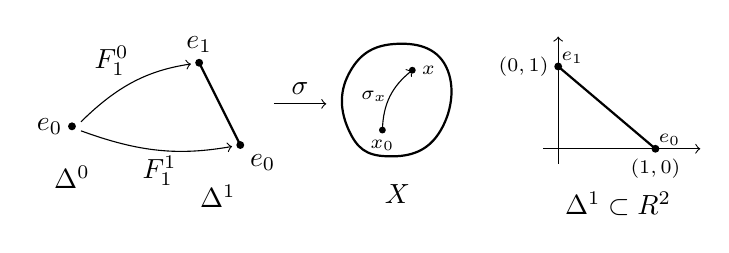
\begin{tikzpicture}[baseline=(current bounding box.center), scale=0.95]
    % Diagrama \Delta^0 -> \Delta^1 -> X
    \coordinate (D0) at (0, 0.5);
    \coordinate (E1) at (1.7, 1.35);
    \coordinate (E0) at (2.25, 0.25);

    \fill (D0) circle (1.5pt) node[left] {$e_0$};
    \node[below] at (0, 0.1) {$\Delta^0$};

    \draw[thick] (E1) -- (E0);
    \fill (E1) circle (1.5pt) node[above] {$e_1$};
    \fill (E0) circle (1.5pt) node[below right] {$e_0$};
    \node[below] at (1.95, -0.15) {$\Delta^1$};

    \draw[->, shorten >=3pt] (0.12, 0.56) to[bend left=18] node[above left, inner sep=2pt] {$F_1^0$} (E1);
    \draw[->, shorten >=3pt] (0.12, 0.44) to[bend right=15] node[below, inner sep=2pt] {$F_1^1$} (E0);

    \draw[->] (2.7, 0.8) -- (3.4, 0.8) node[midway, above] {$\sigma$};

    % Espacio X con trayectoria \sigma_x
    \draw[thick] plot[smooth cycle, tension=0.8] coordinates {(3.7, 0.45) (4.2, 0.1) (4.9, 0.4) (5.0, 1.3) (4.3, 1.6) (3.7, 1.2)};
    \node[below] at (4.35, -0.15) {$X$};

    \coordinate (X0) at (4.15, 0.45);
    \coordinate (XX) at (4.55, 1.25);
    \fill (X0) circle (1.3pt) node[below] {\scriptsize $x_0$};
    \fill (XX) circle (1.3pt) node[right] {\scriptsize $x$};
    \draw[->] (X0) to[bend left=25] node[left, inner sep=1pt] {\scriptsize $\sigma_x$} (XX);

    % Caso \Delta^1 \subset \mathbb{R}^2
    \begin{scope}[xshift=6.5cm, yshift=0.2cm]
        \draw[->] (-0.2, 0) -- (1.9, 0);
        \draw[->] (0, -0.2) -- (0, 1.5);
        \draw[thick] (0, 1.1) -- (1.3, 0);
        \fill (0, 1.1) circle (1.5pt) node[left] {\scriptsize $(0,1)$} node[above right, inner sep=1pt] {\scriptsize $e_1$};
        \fill (1.3, 0) circle (1.5pt) node[below] {\scriptsize $(1,0)$} node[above right, inner sep=1pt] {\scriptsize $e_0$};
        \node[below] at (0.8, -0.45) {$\Delta^1 \subset \mathbb{R}^2$};
    \end{scope}
\end{tikzpicture}
\]
obtenemos
\begin{align*}
\partial_1\left(\sum_\sigma r_\sigma \sigma\right) &= \sum_\sigma r_\sigma \partial_1(\sigma) \\
&= \sum_\sigma r_\sigma (\sigma \circ F_1^0 - \sigma \circ F_1^1) \\
&= \sum_\sigma r_\sigma (\sigma(e_1) - \sigma(e_0)) \\
&= \sum_\sigma r_\sigma \sigma(e_1) - \sum_\sigma r_\sigma \sigma(e_0).
\end{align*}
Por lo tanto,
\[
\varepsilon \partial_1\left(\sum_\sigma r_\sigma \sigma\right) = \varepsilon\left(\sum_\sigma r_\sigma \sigma(e_1) - \sum_\sigma r_\sigma \sigma(e_0)\right) = \sum_\sigma r_\sigma - \sum_\sigma r_\sigma = 0,
\]
de donde $\operatorname{Im} \partial_1 \subset \ker \varepsilon$. (Notemos que esta contención es válida para cualquier espacio $X$.)

Recíprocamente, veamos que $\ker \varepsilon \subset \operatorname{Im} \partial_1$. Sea $\sum_x r_x x \in S_0(X)$ tal que $\sum_x r_x = 0$. Fijemos un punto $x_0 \in X$; como $X$ es $0$-conexo, para cada $x \in X$ podemos tomar una trayectoria $\sigma_x \colon \Delta^1 \to X$ tal que $\sigma_x(e_0) = x_0$ y $\sigma_x(e_1) = x$. Consideremos ahora la $1$-cadena $\sum_x r_x \sigma_x \in S_1(X)$. Entonces,
\begin{align*}
\partial_1\left(\sum_x r_x \sigma_x\right) &= \sum_x r_x (\sigma_x(e_1) - \sigma_x(e_0)) \\
&= \sum_x r_x x - \left(\sum_x r_x\right) x_0 \\
&= \sum_x r_x x - 0 \cdot x_0 = \sum_x r_x x,
\end{align*}
lo que prueba que $\sum_x r_x x \in \operatorname{Im} \partial_1$. Así, $\ker \varepsilon = \operatorname{Im} \partial_1$, y en consecuencia
\[
H_0(X; R) = \raisebox{0.2ex}{$S_0(X)$} \big/ \raisebox{-0.2ex}{$\operatorname{Im} \partial_1$} = \raisebox{0.2ex}{$S_0(X)$} \big/ \raisebox{-0.2ex}{$\ker \varepsilon$} \cong R.
\]
\end{dem}
\begin{definicion}
Sea $\{(C_*^\alpha, \partial_*^\alpha)\}_{\alpha \in \Lambda}$ una familia de complejos de cadenas de $R$-módulos. Definimos el complejo de cadenas $\bigoplus_{\alpha \in \Lambda} C_*^\alpha$ dando en cada grado $q$ el $R$-módulo
\[
\left( \bigoplus_{\alpha \in \Lambda} C_*^\alpha \right)_q = \bigoplus_{\alpha \in \Lambda} C_q^\alpha,
\]
con operador frontera
\[
\partial_q^\oplus \colon \bigoplus_{\alpha \in \Lambda} C_q^\alpha \longrightarrow \bigoplus_{\alpha \in \Lambda} C_{q-1}^\alpha.
\]
Para definir $\partial_q^\oplus$ usamos la propiedad universal de $\bigoplus_{\alpha \in \Lambda} C_q^\alpha$; es decir, consideramos el siguiente diagrama para cada $\alpha \in \Lambda$:
\[
\begin{tikzcd}[column sep=3.2em, row sep=2.8em]
C_q^\alpha \arrow[r, "i_\alpha"] \arrow[d, "\partial_q^\alpha"'] \arrow[dr] & \displaystyle\bigoplus_{\alpha \in \Lambda} C_q^\alpha \arrow[d, dashed, "\partial_q^\oplus"] \\
C_{q-1}^\alpha \arrow[r, "j_\alpha"'] & \displaystyle\bigoplus_{\alpha \in \Lambda} C_{q-1}^\alpha
\end{tikzcd}
\]
Por la propiedad universal, existe un único homomorfismo $\partial_q^\oplus$ que hace conmutar el diagrama (de modo que $\partial_q^\oplus \circ i_\alpha = j_\alpha \circ \partial_q^\alpha$ para todo $\alpha \in \Lambda$). Claramente se cumple que $\partial_{q-1}^\oplus \circ \partial_q^\oplus = 0$.
\end{definicion}
\begin{ejercicio}
    % ID: 68
Ver que se tiene un isomorfismo
\begin{align*}
    \bigoplus_{\alpha \in \Lambda} H_q(C_*^\alpha, \partial_*^\alpha)&\xlongrightarrow[]{\cong} H_q\hspace{0.2mm}\bigg(\displaystyle\bigoplus_{\alpha \in \Lambda} C_*^\alpha, \partial_*^\oplus\bigg)\\
    \{[c_\alpha]\}_{\alpha \in \Lambda}&\longmapsto [\{[c_\alpha]\}_{\alpha \in \Lambda}]
\end{align*}
\end{ejercicio}

\begin{nota}
Consideremos los $R$-módulos libres $R(B_\alpha)$ para $\alpha \in \Lambda$. Entonces
\[
\bigoplus_{\alpha \in \Lambda} R(B_\alpha) \cong R\bigg(\coprod_{\alpha \in \Lambda} B_\alpha\bigg),
\]
y el isomorfismo está dado por la propiedad universal del módulo libre mediante el siguiente diagrama:
\[
\begin{tikzcd}[column sep=2.8em, row sep=2.4em]
\displaystyle\coprod_{\alpha \in \Lambda} B_\alpha \arrow[r, hook] \arrow[dr, "\psi"'] & R\bigg(\displaystyle\coprod_{\alpha \in \Lambda} B_\alpha\bigg) \arrow[d, dashed, "\overline{\psi}"] \\
& \displaystyle\bigoplus_{\alpha \in \Lambda} R(B_\alpha)
\end{tikzcd}
\]
donde $\psi$ se define como
\[
\psi(b, \alpha)(\beta) =
\begin{cases}
    1b, & \text{si } \beta = \alpha, \\
    0, & \text{si } \beta \neq \alpha,
\end{cases}
\]
la cual induce el isomorfismo $\overline{\psi}$.
\end{nota}

\begin{corolario}
Sea $X$ un espacio triangulable tal que $|K| \cong X$, donde $\dim K = n$. Entonces $H_q(X; R) \cong 0$ para todo $q > n$.
\end{corolario}

\begin{dem}
Tenemos que $C_q^<(K; R) = 0$ si $q > n$. Por lo tanto,
\[
0 \cong H_q(C_*^<(K; R)) \underset{\varphi}{\cong} H_q(|K|; R) \cong H_q(X; R).
\]
\end{dem}
\begin{prop}
Sea $X$ un espacio y sea $\{X_\alpha\}_{\alpha \in \Lambda}$ la familia de componentes por trayectorias de $X$. Entonces
\[
H_q(X; R) \cong \bigoplus_{\alpha \in \Lambda} H_q(X_\alpha; R),
\]
donde el isomorfismo está inducido por los homomorfismos $i_{\alpha*} \colon H_q(X_\alpha; R) \to H_q(X; R)$ y $i_\alpha \colon X_\alpha \hookrightarrow X$ es la inclusión.
\end{prop}

\begin{dem}
Para cada $\alpha \in \Lambda$, la inclusión $i_\alpha \colon X_\alpha \hookrightarrow X$ induce el homomorfismo de cadenas $i_{\alpha\#} \colon S_q(X_\alpha) \to S_q(X)$. Consideremos el siguiente diagrama:
\[
\begin{tikzcd}[column sep=3.4em, row sep=2.6em]
S_q(X_\alpha) \arrow[r, "\iota_\alpha"] \arrow[dr, "i_{\alpha\#}"'] & \displaystyle\bigoplus_{\alpha \in \Lambda} S_q(X_\alpha) \arrow[d, dashed, "{\bigoplus_{\alpha \in \Lambda} i_{\alpha\#}}"] \\
& S_q(X)
\end{tikzcd}
\]
Por la propiedad universal de la suma directa, existe un único homomorfismo $\bigoplus_{\alpha \in \Lambda} i_{\alpha\#}$ que hace conmutar el triángulo para cada $\alpha \in \Lambda$.

Vamos a ver que $\bigoplus_{\alpha \in \Lambda} i_{\alpha\#}$ es un isomorfismo. Por definición, $S_q(X) = R(\mathcal{S}_q(X))$, donde $\mathcal{S}_q(X) = \{\sigma \colon \Delta^q \to X \mid \sigma \text{ es continua}\}$. Por la nota anterior, la base de $\bigoplus_{\alpha \in \Lambda} S_q(X_\alpha)$ es $\coprod_{\alpha \in \Lambda} \mathcal{S}_q(X_\alpha)$. Así, para ver que estos dos módulos libres son isomorfos basta verificar que las inclusiones $i_\alpha \colon X_\alpha \hookrightarrow X$ inducen una biyección entre sus bases:
\[
\coprod_{\alpha \in \Lambda} \tilde{i}_\alpha \colon \coprod_{\alpha \in \Lambda} \mathcal{S}_q(X_\alpha) \longrightarrow \mathcal{S}_q(X), \; \text{donde } \tilde{i}_\alpha(\sigma) = i_\alpha \circ \sigma.
\]
\[
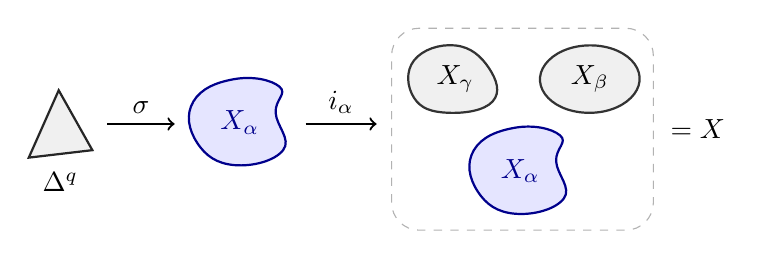
\begin{tikzpicture}[baseline=(current bounding box.center), scale=0.95]
    % Simplejo \Delta^q
    \fill[gray!12] (-0.4, 0.55) -- (0.45, 0.65) -- (0.0, 1.45) -- cycle;
    \draw[thick, black!85] (-0.4, 0.55) -- (0.45, 0.65) -- (0.0, 1.45) -- cycle;
    \node[below] at (0.02, 0.48) {$\Delta^q$};

    % Flecha \sigma
    \draw[->, thick] (0.65, 1.0) -- (1.55, 1.0) node[midway, above] {$\sigma$};

    % Componente aislada X_\alpha
    \fill[blue!10] plot[smooth cycle, tension=0.75] coordinates {
        (1.85, 0.75) (2.35, 0.45) (3.0, 0.65) (2.9, 1.15) (2.95, 1.5) (2.35, 1.6) (1.8, 1.3)
    };
    \draw[thick, blue!55!black] plot[smooth cycle, tension=0.75] coordinates {
        (1.85, 0.75) (2.35, 0.45) (3.0, 0.65) (2.9, 1.15) (2.95, 1.5) (2.35, 1.6) (1.8, 1.3)
    };
    \node[blue!55!black] at (2.42, 1.02) {$X_\alpha$};

    % Flecha de inclusión i_\alpha
    \draw[->, thick] (3.3, 1.0) -- (4.25, 1.0) node[midway, above] {$i_\alpha$};

    % Agrupación del espacio X
    \draw[dashed, gray!60, rounded corners=10pt] (4.45, -0.42) rectangle (7.95, 2.28);

    % Componente X_\gamma
    \fill[gray!12] plot[smooth cycle, tension=0.75] coordinates {
        (4.75, 1.35) (5.2, 1.15) (5.8, 1.3) (5.75, 1.75) (5.3, 2.05) (4.75, 1.85)
    };
    \draw[thick, black!80] plot[smooth cycle, tension=0.75] coordinates {
        (4.75, 1.35) (5.2, 1.15) (5.8, 1.3) (5.75, 1.75) (5.3, 2.05) (4.75, 1.85)
    };
    \node at (5.3, 1.6) {$X_\gamma$};

    % Componente X_\beta
    \fill[gray!12] plot[smooth cycle, tension=0.75] coordinates {
        (6.5, 1.4) (7.05, 1.15) (7.65, 1.35) (7.7, 1.8) (7.15, 2.05) (6.55, 1.85)
    };
    \draw[thick, black!80] plot[smooth cycle, tension=0.75] coordinates {
        (6.5, 1.4) (7.05, 1.15) (7.65, 1.35) (7.7, 1.8) (7.15, 2.05) (6.55, 1.85)
    };
    \node at (7.1, 1.6) {$X_\beta$};

    % Componente X_\alpha dentro de X
    \fill[blue!10] plot[smooth cycle, tension=0.75] coordinates {
        (5.6, 0.1) (6.1, -0.2) (6.75, 0.0) (6.65, 0.5) (6.7, 0.85) (6.1, 0.95) (5.55, 0.65)
    };
    \draw[thick, blue!55!black] plot[smooth cycle, tension=0.75] coordinates {
        (5.6, 0.1) (6.1, -0.2) (6.75, 0.0) (6.65, 0.5) (6.7, 0.85) (6.1, 0.95) (5.55, 0.65)
    };
    \node[blue!55!black] at (6.17, 0.37) {$X_\alpha$};

    \node[right] at (8.05, 0.93) {$= X$};
\end{tikzpicture}
\]

\begin{itemize}
    \item \textit{Suprayectividad:} Dada una función continua $\tau \colon \Delta^q \to X$, como $\Delta^q$ es $0$-conexo, se tiene que $\tau(\Delta^q) \subset X_\alpha$ para alguna $\alpha \in \Lambda$. Por lo tanto, existe una función continua $\tau' \colon \Delta^q \to X_\alpha$ tal que conmuta el diagrama
    \[
    \begin{tikzcd}[column sep=2.2em, row sep=2.2em]
    & X_\alpha \arrow[dr, hook, "i_\alpha"] & \\
    \Delta^q \arrow[ur, "\tau'"] \arrow[rr, "\tau"'] & & X
    \end{tikzcd}
    \]
    es decir, $\tau = i_\alpha \circ \tau' = \tilde{i}_\alpha(\tau')$.

    \item \textit{Inyectividad:} Sean $\sigma, \tau \in \coprod_{\alpha \in \Lambda} \mathcal{S}_q(X_\alpha)$. Si primero suponemos que $\sigma, \tau \in \mathcal{S}_q(X_\alpha)$, entonces $i_\alpha \circ \sigma = i_\alpha \circ \tau$ implica $\sigma = \tau$, pues $i_\alpha$ es inyectiva. Ahora, si $\sigma \in \mathcal{S}_q(X_\alpha)$ y $\tau \in \mathcal{S}_q(X_\beta)$ satisfacen $i_\alpha \circ \sigma = i_\beta \circ \tau$, entonces $\sigma(t) = \tau(t) \in X_\alpha \cap X_\beta$ para todo $t \in \Delta^q$. Si $\alpha \neq \beta$, esto es una contradicción pues las componentes por trayectorias son ajenas; luego $\alpha = \beta$ y regresamos al caso anterior.
\end{itemize}

Por consiguiente, $S_*(X) \cong \bigoplus_{\alpha \in \Lambda} S_*(X_\alpha)$ como complejos de cadenas. Aplicando homología obtenemos:
\begin{align*}
H_q(X; R) &\equiv H_q(S_*(X)) \\
&\cong H_q\!\left(\bigoplus_{\alpha \in \Lambda} S_*(X_\alpha)\right) \\
&\cong \bigoplus_{\alpha \in \Lambda} H_q(S_*(X_\alpha))  \\
&= \bigoplus_{\alpha \in \Lambda} H_q(X_\alpha; R).
\end{align*}
de donde $H_q(X; R) \cong \bigoplus_{\alpha \in \Lambda} H_q(X_\alpha; R)$.
\end{dem}

\begin{coro}
Sea $X$ un espacio; entonces $H_0(X; R)$ es isomorfo a una suma directa de copias de $R$, una por cada componente por trayectorias de $X$.
\end{coro}

\begin{dem}
Sea $\{X_\alpha\}_{\alpha \in \Lambda}$ la familia de componentes por trayectorias de $X$. Por la proposición anterior y el resultado para espacios $0$-conexos, se tiene
\[
H_0(X; R) \cong \bigoplus_{\alpha \in \Lambda} H_0(X_\alpha; R) \cong \bigoplus_{\alpha \in \Lambda} R.
\]
\end{dem}

\begin{definicion}[Primera definición. Homología relativa]
Sea $(X, A)$ una pareja de espacios. La inclusión $i \colon A \hookrightarrow X$ induce un monomorfismo $i_\# \colon S_q(A) \hookrightarrow S_q(X)$, por lo que identificamos a $S_q(A)$ como un submódulo de $S_q(X)$. Además, el operador frontera $\partial_q$ se restringe a $S_q(A)$ haciendo conmutar el siguiente diagrama:
\[
\begin{tikzcd}[column sep=2.6em, row sep=2.4em]
S_q(X) \arrow[r, "\partial_q"] & S_{q-1}(X) \\
S_q(A) \arrow[u, hook, "i_\#"] \arrow[r, dashed, "\partial_q|"'] & S_{q-1}(A) \arrow[u, hook, "i_\#"']
\end{tikzcd}
\]
ya que, para cada $\sigma \in \mathcal{S}_q(A)$, tenemos
\[
\begin{tikzcd}[column sep=2.4em, row sep=2.2em]
\Delta^q \arrow[r, "\sigma"] & A \\
\Delta^{q-1} \arrow[u, "F_q^i"] \arrow[ur, "\sigma \circ F_q^i"'] &
\end{tikzcd}
\hspace{2.5em}
\partial_q(\sigma) = \sum_{i=0}^q (-1)^i \sigma \circ F_q^i,
\]
con $(\sigma \circ F_q^i)(\Delta^{q-1}) \subset A$.

Por lo tanto, al pasar al cociente obtenemos el \textit{complejo de cadenas relativas} $(S_*(X, A), \bar{\partial}_*)$ dado en cada grado por
\[
\begin{tikzcd}[column sep=0.5em, row sep=2.2em]
S_q(X, A) \arrow[r, phantom, "\equiv"] &[-0.1cm] \raisebox{0.2ex}{$S_q(X)$} / \raisebox{-0.2ex}{$S_q(A)$} \arrow[d, "\bar{\partial}_q"] \\
S_{q-1}(X, A) \arrow[r, phantom, "\equiv"] & \raisebox{0.2ex}{$S_{q-1}(X)$} / \raisebox{-0.2ex}{$S_{q-1}(A)$}
\end{tikzcd}
\]
Definimos la \textit{homología relativa} de la pareja $(X, A)$ con coeficientes en $R$ como
\[
H_q(X, A; R) \equiv H_q(S_*(X, A), \bar{\partial}_*).
\]
\end{definicion}

%%%% Clase 34 del 28/10/26 inciada el 18/11/26 terminada el 22/11/2026

%%%%%% Clase 35 del 30/10/2026 iniciada el 22/11/2026

\begin{definicion}[Segunda definición. Homología relativa]
Sea $(X, A)$ una pareja de espacios. Por analogía con los $R$-módulos de $q$-ciclos y $q$-fronteras de $X$,
\begin{align*}
Z_q(X) &= \{ c \in S_q(X) \mid \partial_q(c) = 0 \}, \\
B_q(X) &= \{ \partial_{q+1}(c') \mid c' \in S_{q+1}(X) \},
\end{align*}
definimos los $R$-módulos de \textit{$q$-ciclos relativos} y \textit{$q$-fronteras relativas} de la pareja $(X, A)$ como
\begin{align*}
Z_q(X, A) &= \{ c \in S_q(X) \mid \partial_q(c) \in S_{q-1}(A) \}, \\
B_q(X, A) &= \{ c \in S_q(X) \mid c = \partial_{q+1}(c') + d, \; \text{con } c' \in S_{q+1}(X) \text{ y } d \in S_q(A) \}.
\end{align*}
Observemos que $B_q(X, A) \subset Z_q(X, A)$: en efecto, si $c = \partial_{q+1}(c') + d \in B_q(X, A)$ con $c' \in S_{q+1}(X)$ y $d \in S_q(A)$, entonces
\[
\partial_q(c) = \partial_q \partial_{q+1}(c') + \partial_q(d) = \partial_q(d) \in S_{q-1}(A),
\]
ya que $\partial_q \circ \partial_{q+1} = 0$ y $\partial_q(S_q(A)) \subset S_{q-1}(A)$.

Por lo tanto, el cociente está bien definido y definimos la \textit{homología relativa} de la pareja $(X, A)$ con coeficientes en $R$ como
\[
H_q(X, A; R) \equiv \raisebox{0.2ex}{$Z_q(X, A)$} / \raisebox{-0.2ex}{$B_q(X, A)$}.
\]
\end{definicion}

\begin{nota}
Si $X = \emptyset$, entonces $S_q(X) = 0$ para todo $q$.
\end{nota}

\begin{ejercicio}
    % ID: 69
Ver que las dos definiciones de $H_q(X, A; R)$ son isomorfas.
\end{ejercicio}

\begin{definicion}
Una \textit{función continua de parejas} $f \colon (X, A) \to (Y, B)$ es una función continua $f \colon X \to Y$ tal que $f(A) \subset B$.
\end{definicion}

Dada una función continua de parejas $f \colon (X, A) \to (Y, B)$, podemos describir el homomorfismo inducido en homología relativa a partir de cualquiera de las dos definiciones anteriores:

\begin{itemize}
    \item \textbf{A partir de la primera definición:} Consideramos el morfismo de cadenas inducido $f_\# \colon S_q(X) \to S_q(Y)$. Como $f(A) \subset B$, se cumple que $f_\#(S_q(A)) \subset S_q(B)$, por lo que $f_\#$ pasa a los cocientes induciendo un homomorfismo $\bar{f}_\#$ que hace conmutar el siguiente diagrama:
    \[
    \begin{tikzcd}[column sep=2.6em, row sep=2.4em]
    &[-0.8cm] S_q(X) \arrow[r, "f_\#"] \arrow[d] & S_q(Y) \arrow[d] &[-0.8cm] \\
    S_q(X, A) \arrow[r, phantom, "\equiv"] & S_q(X)/S_q(A) \arrow[r, "\bar{f}_\#"'] & S_q(Y)/S_q(B) \arrow[r, phantom, "\equiv"] & S_q(Y, B)
    \end{tikzcd}
    \]
\end{itemize}

\begin{ejercicio}
    % ID: 70
Ver que $\bar{f}_\# \colon (S_*(X, A), \bar{\partial}_*) \to (S_*(Y, B), \bar{\partial}'_*)$ es un morfismo de cadenas.
\end{ejercicio}

\begin{itemize}
    \item \textbf{A partir de la segunda definición:} Consideramos el morfismo de cadenas $f_\# \colon (S_*(X), \partial_*) \to (S_*(Y), \partial'_*)$ y verificamos que preserva ciclos y fronteras relativos:
    \begin{enumerate}
        \item \textit{Preservación de ciclos relativos ($f_\#(Z_q(X, A)) \subset Z_q(Y, B)$):} Sea $c \in Z_q(X, A)$, de modo que $\partial_q(c) \in S_{q-1}(A)$. Como $f_\#$ es un morfismo de cadenas, tenemos
        \[
        \partial'_q(f_\#(c)) = f_\#(\partial_q(c)).
        \]
        Puesto que $f(A) \subset B$ y $\partial_q(c) \in S_{q-1}(A)$, se tiene que $f_\#(\partial_q(c)) \in S_{q-1}(B)$; por lo tanto, $f_\#(c) \in Z_q(Y, B)$.

        \item \textit{Preservación de fronteras relativas ($f_\#(B_q(X, A)) \subset B_q(Y, B)$):} Sea $c \in B_q(X, A)$, entonces $c = \partial_{q+1}(c') + d$ con $c' \in S_{q+1}(X)$ y $d \in S_q(A)$. Usando la conmutatividad del diagrama
        \[
        \begin{tikzcd}[column sep=2.8em, row sep=2.4em]
        S_{q+1}(X) \arrow[r, "\partial_{q+1}"] \arrow[d, "f_\#"'] & S_q(X) \arrow[d, "f_\#"] \\
        S_{q+1}(Y) \arrow[r, "\partial'_{q+1}"'] & S_q(Y)
        \end{tikzcd}
        \]
        obtenemos
        \[
        f_\#(c) = f_\#(\partial_{q+1}(c')) + f_\#(d) = \partial'_{q+1}(f_\#(c')) + f_\#(d).
        \]
        Como $f_\#(c') \in S_{q+1}(Y)$ y $f_\#(d) \in S_q(B)$, concluimos que $f_\#(c) \in B_q(Y, B)$.
    \end{enumerate}
    En consecuencia, $f_\#$ induce el homomorfismo
    \[
    f_* \colon H_q(X, A; R) \equiv Z_q(X, A)/B_q(X, A) \longrightarrow H_q(Y, B; R) \equiv Z_q(Y, B)/B_q(Y, B),
    \]
    dado por $f_*([c]) = [f_\#(c)]$.
\end{itemize}
\begin{nota}
El complejo de cadenas relativas $S_q(X, A) \equiv S_q(X)/S_q(A)$ está formado por $R$-módulos libres, ya que la base de $S_q(A)$ es un subconjunto de la base de $S_q(X)$. En consecuencia, la base de $S_q(X)/S_q(A)$ está formada por (las clases de) los $q$-simplejos singulares $\sigma \colon \Delta^q \to X$ tales que $\sigma(\Delta^q) \not\subset A$.
\end{nota}

\begin{prop}
Sea $(X, A)$ una pareja de espacios. Denotemos por $\{X_\alpha\}_{\alpha \in \Lambda}$ a la familia de componentes por trayectorias de $X$ y sea $A_\alpha = X_\alpha \cap A$. Entonces las inclusiones $i_\alpha \colon (X_\alpha, A_\alpha) \hookrightarrow (X, A)$ inducen un isomorfismo
\[
\bigoplus_{\alpha \in \Lambda} H_q(X_\alpha, A_\alpha; R) \xrightarrow{\;\bigoplus_\alpha i_{\alpha*}\;} H_q(X, A; R).
\]
\end{prop}

\begin{dem}
Para cada $\alpha \in \Lambda$, consideremos el diagrama conmutativo de inclusiones y el diagrama inducido en los complejos de cadenas singulares:
\[
\begin{tikzcd}[column sep=2.6em, row sep=2.2em]
X_\alpha \arrow[r, hook, "i_\alpha"] & X \\
A_\alpha \arrow[u, hook] \arrow[r, hook] & A \arrow[u, hook]
\end{tikzcd}
\hspace{2em} \Longrightarrow \hspace{2em}
\begin{tikzcd}[column sep=2.6em, row sep=2.2em]
S_*(X_\alpha) \arrow[r, "i_{\alpha\#}"] & S_*(X) \\
S_*(A_\alpha) \arrow[u, hook] \arrow[r, hook] & S_*(A) \arrow[u, hook]
\end{tikzcd}
\]
Al pasar a los cocientes, cada $i_{\alpha\#}$ induce un morfismo de cadenas
\[
\bar{i}_{\alpha\#} \colon S_*(X_\alpha)/S_*(A_\alpha) \longrightarrow S_*(X)/S_*(A).
\]
Por la propiedad universal de la suma directa, obtenemos un único morfismo de cadenas
\[
\bigoplus_{\alpha \in \Lambda} \bar{i}_{\alpha\#} \colon \bigoplus_{\alpha \in \Lambda} S_*(X_\alpha)/S_*(A_\alpha) \longrightarrow S_*(X)/S_*(A).
\]

Por la nota anterior y la propiedad de las sumas directas de $R$-módulos libres, en cada grado $q$ las bases del dominio y del codominio están dadas respectivamente por
\[
\coprod_{\alpha \in \Lambda} \{ \sigma \colon \Delta^q \to X_\alpha \mid \sigma(\Delta^q) \not\subset A_\alpha \}
\; \text{ y } \;
\{ \tau \colon \Delta^q \to X \mid \tau(\Delta^q) \not\subset A \},
\]
y la función inducida entre las bases es $\coprod_{\alpha \in \Lambda} \tilde{i}_\alpha$, donde $\tilde{i}_\alpha(\sigma) = i_\alpha \circ \sigma$.

Veamos que $\coprod_{\alpha \in \Lambda} \tilde{i}_\alpha$ es suprayectiva. Sea $\tau \colon \Delta^q \to X$ continua tal que $\tau(\Delta^q) \not\subset A$. Como $\Delta^q$ es $0$-conexo, existe una componente por trayectorias $X_\alpha$ y una función continua $\tau' \colon \Delta^q \to X_\alpha$ que hace conmutar el siguiente diagrama:
\[
\begin{tikzcd}[column sep=2.6em, row sep=2.2em]
& X_\alpha \arrow[d, hook, "i_\alpha"] \\
\Delta^q \arrow[ur, dashed, "\tau'"] \arrow[r, "\tau"'] & X
\end{tikzcd}
\]
es decir, $i_\alpha \circ \tau' = \tau$. Además, $\tau'(\Delta^q) \not\subset A_\alpha = X_\alpha \cap A$, ya que si $\tau'(\Delta^q) \subset A_\alpha$, entonces $\tau(\Delta^q) \subset A_\alpha \subset A$, lo cual es una contradicción. Por lo tanto, $\tilde{i}_\alpha(\tau') = \tau$.

La inyectividad de $\coprod_{\alpha \in \Lambda} \tilde{i}_\alpha$ se deja como el ejercicio siguiente. Así, $\bigoplus_{\alpha \in \Lambda} \bar{i}_{\alpha\#}$ es un isomorfismo de complejos de cadenas. Aplicando homología y usando que esta conmuta con la suma directa de complejos de cadenas, se obtiene el resultado.
\end{dem}

\begin{ejercicio}
    % ID: 71
Ver que la función $\coprod_{\alpha \in \Lambda} \tilde{i}_\alpha$ de la demostración anterior es inyectiva.
\end{ejercicio}

\begin{prop}
Sea $X$ un espacio $0$-conexo y $A \subset X$ con $A \neq \emptyset$. Entonces $H_0(X, A; R) \cong 0$.
\end{prop}

\begin{dem}
Recordemos que $H_0(X, A; R) = Z_0(X, A)/B_0(X, A)$, donde
\begin{align*}
Z_0(X, A) &= \{ c \in S_0(X) \mid \underbrace{\partial_0(c)}_{=\;0} \in \underbrace{S_{-1}(A)}_{=\;0} \} = S_0(X), \\
B_0(X, A) &= \{ c \in S_0(X) \mid c = \partial_1(c') + d, \; \text{con } c' \in S_1(X) \text{ y } d \in S_0(A) \}.
\end{align*}
Sea $\sum_{x \in X} r_x x \in S_0(X)$ y fijemos un punto $x_0 \in A$. Como $X$ es $0$-conexo, para cada $x \in X$ existe una trayectoria $\sigma_x \colon \Delta^1 \to X$ tal que $\sigma_x(e_0) = x_0$ y $\sigma_x(e_1) = x$. Tomemos la $1$-cadena $\sum_{x \in X} r_x \sigma_x \in S_1(X)$; su frontera es
\begin{align*}
\partial_1\left(\sum_{x \in X} r_x \sigma_x\right) &= \sum_{x \in X} r_x \partial_1(\sigma_x) = \sum_{x \in X} r_x (\sigma_x(e_1) - \sigma_x(e_0)) \\
&= \sum_{x \in X} r_x (x - x_0) = \sum_{x \in X} r_x x - \left(\sum_{x \in X} r_x\right) x_0.
\end{align*}
Despejando, obtenemos
\[
\sum_{x \in X} r_x x = \partial_1\left(\sum_{x \in X} r_x \sigma_x\right) + \left(\sum_{x \in X} r_x\right) x_0 \in B_0(X, A),
\]
ya que $\left(\sum_{x \in X} r_x\right) x_0 \in S_0(A)$. Por lo tanto, $Z_0(X, A) = S_0(X) \subset B_0(X, A)$, de donde
\[
H_0(X, A; R) = Z_0(X, A)/B_0(X, A) \cong 0.
\]
\end{dem}

\begin{prop}
Sea $(X, A)$ una pareja de espacios; entonces $H_0(X, A; R)$ es isomorfo a una suma directa de copias de $R$, una copia por cada componente por trayectorias de $X$ que \textit{no} intersecta a $A$.
\end{prop}

\begin{dem}
Sean $\{X_\alpha\}_{\alpha \in \Lambda}$ las componentes por trayectorias de $X$ y sea $A_\alpha = X_\alpha \cap A$. Por un resultado anterior, tenemos
\[
H_0(X, A; R) \cong \bigoplus_{\alpha \in \Lambda} H_0(X_\alpha, A_\alpha; R).
\]
Por la proposición anterior, si $A_\alpha \neq \emptyset$, entonces $H_0(X_\alpha, A_\alpha; R) \cong 0$. Por otro lado, si $A_\alpha = \emptyset$, entonces $S_*(X_\alpha, \emptyset) = S_*(X_\alpha)$ y, al ser $X_\alpha$ un espacio $0$-conexo, se cumple que 
$$H_0(X_\alpha, \emptyset; R) = H_0(X_\alpha; R) \cong R.$$ 
En consecuencia, la suma directa conserva exactamente una copia de $R$ por cada componente $X_\alpha$ tal que $X_\alpha \cap A = \emptyset$.
\end{dem}
\begin{teorema}
Sea $(X, A)$ una pareja de espacios. Entonces existe una sucesión exacta larga en homología
\begin{align*}
\cdots &\longrightarrow H_q(A; R) \xrightarrow{\;i_*\;} H_q(X; R) \xrightarrow{\;j_*\;} H_q(X, A; R) \xrightarrow{\;\hat{\partial}_q\;} H_{q-1}(A; R) \\
&\xrightarrow{\;i_*\;} H_{q-1}(X; R) \longrightarrow \cdots \longrightarrow H_0(X; R) \xrightarrow{\;j_*\;} H_0(X, A; R) \longrightarrow 0,
\end{align*}
donde $i \colon A \hookrightarrow X$ y $j \colon X \hookrightarrow (X, A)$ son las inclusiones, y $\hat{\partial}_q$ está definido por
\[
\hat{\partial}_q([c]) = [\partial_q(c)].
\]
\end{teorema}

\begin{dem}
Veamos primero que $\hat{\partial}_q$ está bien definido. Si $[c] \in H_q(X, A; R)$, entonces $c \in Z_q(X, A)$, de modo que $\partial_q(c) \in S_{q-1}(A)$ y $\partial_{q-1}(\partial_q(c)) = 0$; así, $\partial_q(c) \in Z_{q-1}(A)$ y $[\partial_q(c)] \in H_{q-1}(A; R)$.

Para verificar que no depende del representante, supongamos que $[c] = [\tilde{c}]$ en $H_q(X, A; R)$. Entonces $\tilde{c} - c \in B_q(X, A)$, por lo que existen $c' \in S_{q+1}(X)$ y $d \in S_q(A)$ tales que
\[
\tilde{c} - c = \partial_{q+1}(c') + d.
\]
Aplicando $\partial_q$, obtenemos
\[
\partial_q(\tilde{c}) - \partial_q(c) = \partial_q \partial_{q+1}(c') + \partial_q(d) = \partial_q(d),
\]
donde $d \in S_q(A)$, es decir, $\partial_q(\tilde{c}) - \partial_q(c) \in B_{q-1}(A)$. Por lo tanto,
\[
[\partial_q(\tilde{c})] = [\partial_q(c)] \in H_{q-1}(A; R).
\]


%%%% Clase 35 del 30/10/26 inciada el 22/11/26 terminada el 22/11/2026

%%%%%% Clase 36 del 02/11/2026 iniciada el 22/11/2026

Verificamos ahora la exactitud de la sucesión en cada término:

\begin{itemize}
    \item {Exactitud en $H_q(X; R)$:} Recordemos que $j_* \colon Z_q(X)/B_q(X) \to Z_q(X, A)/B_q(X, A)$, donde
    \begin{align*}
    Z_q(X, A) &= \{ c \in S_q(X) \mid \partial_q(c) \in S_{q-1}(A) \}, \\
    B_q(X, A) &= \{ c \in S_q(X) \mid c = \partial_{q+1}(c') + i_\#(d), \; c' \in S_{q+1}(X), \; d \in S_q(A) \}.
    \end{align*}
    Sea $[z] \in H_q(A; R)$; entonces
    \[
    j_* i_*([z]) = [i_\#(z)] = 0 \in H_q(X, A; R),
    \]
    ya que $i_\#(z) \in i_\#(S_q(A)) \subset B_q(X, A)$. Por lo tanto, $\operatorname{Im} i_* \subset \ker j_*$.

    Recíprocamente, sea $[z] \in H_q(X; R)$ tal que $j_*([z]) = 0 \in H_q(X, A; R)$. Entonces $z \in B_q(X, A)$, de modo que existen $c' \in S_{q+1}(X)$ y $d \in S_q(A)$ tales que
    \[
    z = \partial_{q+1}(c') + i_\#(d).
    \]
    Como $\partial_q(z) = 0$ y $\partial_q \partial_{q+1}(c') = 0$, se tiene $i_\#(\partial_q(d)) = \partial_q(i_\#(d)) = 0$; al ser $i_\#$ inyectivo, $\partial_q(d) = 0$, luego $[d] \in H_q(A; R)$. Además, $z - i_\#(d) = \partial_{q+1}(c') \in B_q(X)$, por lo que
    \[
    [z] = [i_\#(d)] = i_*([d]).
    \]
    Así, $\ker j_* \subset \operatorname{Im} i_*$.

    \item {Exactitud en $H_q(X, A; R)$:} Sea $[z] \in H_q(X; R)$; entonces
    \[
    \hat{\partial}_q j_*([z]) = \hat{\partial}_q([z]) = [\partial_q(z)] = 0,
    \]
    ya que $z$ es un ciclo. Luego, $\operatorname{Im} j_* \subset \ker \hat{\partial}_q$.

    Recíprocamente, sea $[c] \in H_q(X, A; R)$ tal que $0 = \hat{\partial}_q([c]) = [\partial_q(c)] \in H_{q-1}(A; R)$. Entonces $\partial_q(c) \in B_{q-1}(A)$, es decir, existe $d \in S_q(A)$ tal que $\partial_q(c) = \partial_q(d)$. Por lo tanto, $\partial_q(c - d) = 0$, de donde $[c - d] \in H_q(X; R)$. Finalmente,
    \[
    j_*([c - d]) = [c - d] = [c] \in H_q(X, A; R),
    \]
    ya que $c - (c - d) = d \in S_q(A) \subset B_q(X, A)$. Así, $\ker \hat{\partial}_q \subset \operatorname{Im} j_*$.
\end{itemize}

La verificación de la exactitud en $H_q(A; R)$ se deja como ejercicio.
\end{dem}

\begin{ejercicio}
    % ID: 72
Ver la exactitud de la sucesión larga en $H_q(A; R)$.
\end{ejercicio}

\begin{nota}
Al final de la sucesión exacta larga tenemos
\[
\begin{tikzcd}[column sep=2.2em, row sep=1.2em]
H_0(X; R) \arrow[r, "j_*"] \arrow[d, phantom, "="{description, sloped, inner sep=1pt}] & H_0(X, A; R) \arrow[r] \arrow[d, phantom, "="{description, sloped, inner sep=1pt}] & 0 \\
S_0(X)/\operatorname{Im} \partial_1 & S_0(X)/B_0(X, A) &
\end{tikzcd}
\]
donde $B_0(X, A) = \{ c \in S_0(X) \mid c = \partial_1(c') + d, \; c' \in S_1(X), \; d \in S_0(A) \}$. Como $\operatorname{Im} \partial_1 \subset B_0(X, A)$ y $j_*([c]_{\operatorname{Im} \partial_1}) = [c]_{B_0(X, A)}$, concluimos que $j_*$ es suprayectiva.
\end{nota}

\begin{prop}[Hurewicz]
Sea $X$ un espacio $0$-conexo basado (con punto base $x_0$). Existe un homomorfismo suprayectivo
\[
h \colon \pi_1(X, x_0) \longrightarrow H_1(X; \mathbb{Z}),
\]
dado por $h\langle \alpha \rangle = [\alpha]$ (usando la identificación $\Delta^1 = I$), cuyo núcleo es el subgrupo conmutador de $\pi_1(X, x_0)$. Por lo tanto, $H_1(X; \mathbb{Z})$ es la abelianización de $\pi_1(X, x_0)$.
\end{prop}

\subsection{Cadenas homotópicas}

\begin{nota}
Sea $W$ un espacio vectorial real. Un subconjunto $C \subset W$ es \textit{convexo} si y solo si para cualesquiera $w_0, w_1, \dots, w_q \in C$ y escalares $t_i \geq 0$ ($i = 0, 1, \dots, q$) tales que $\sum_{i=0}^q t_i = 1$, se cumple que la \textit{combinación convexa} de estos puntos pertenece a $C$:
\[
\sum_{i=0}^q t_i w_i \in C.
\]
\end{nota}
\begin{definicion}
Sea $C \subset W$ un conjunto convexo. Una $q$-cadena $\sum_\sigma r_\sigma \sigma \in S_q(C)$ es \textit{afín} si cada $\sigma \colon \Delta^q \to C$ es una función afín; en otras palabras, existen puntos $w_0, w_1, \dots, w_q \in C$ tales que $\sigma$ es el $q$-simplejo singular determinado por $\sigma(e_i) = w_i$ ($0 \leq i \leq q$), es decir,
\[
\sigma\Big(\sum_{j=0}^q t_j e_j\Big) = \sum_{j=0}^q t_j w_j
\]
para todo $\sum_{j=0}^q t_j e_j \in \Delta^q$. En el caso $\Delta^q \subset \mathbb{R}^{q+1}$, esto se escribe simplemente como
\[
\sigma(t_0, \dots, t_q) = \sum_{j=0}^q t_j w_j.
\]
Denotamos a este $q$-simplejo afín por $\sigma = \langle\!\langle w_0, w_1, \dots, w_q \rangle\!\rangle$.
\end{definicion}

\begin{ejercicio}
    % ID: 73
Ver que, para cada $0 \leq i \leq q$, la $i$-cara de $\sigma = \langle\!\langle w_0, w_1, \dots, w_q \rangle\!\rangle$, definida como $\sigma^{(i)} \equiv \sigma \circ F_q^i$, está dada por
\[
\sigma^{(i)} = \langle\!\langle w_0, w_1, \dots, \hat{w}_i, \dots, w_q \rangle\!\rangle.
\]
\end{ejercicio}

\begin{definicion}[Construcción cono]
Dados $w \in C$ y un $q$-simplejo afín $\sigma = \langle\!\langle w_0, w_1, \dots, w_q \rangle\!\rangle$, definimos el $(q+1)$-simplejo afín $w \cdot \sigma$ mediante
\[
w \cdot \sigma \equiv \langle\!\langle w, w_0, w_1, \dots, w_q \rangle\!\rangle.
\]
\end{definicion}
\begin{ejemplo}
Para un $1$-simplejo afín $\sigma = \langle\!\langle w_0, w_1 \rangle\!\rangle$ y un punto $w \in C$, la construcción cono $w \cdot \sigma = \langle\!\langle w, w_0, w_1 \rangle\!\rangle$ se ilustra como sigue:
\[
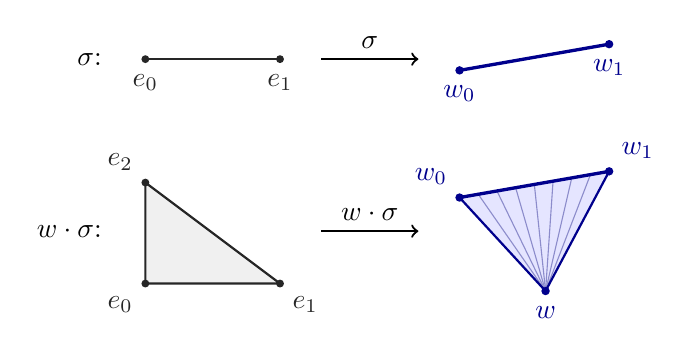
\begin{tikzpicture}[baseline=(current bounding box.center), scale=0.95]
    % --- Fila superior: 1-simplejo \sigma ---
    \node[left] at (-0.45, 3.0) {$\sigma\colon$};

    \coordinate (A0) at (0, 3.0);
    \coordinate (A1) at (1.8, 3.0);
    \draw[thick, black!85] (A0) -- (A1);
    \fill[black!85] (A0) circle (1.5pt) node[below=2pt] {$e_0$};
    \fill[black!85] (A1) circle (1.5pt) node[below=2pt] {$e_1$};

    \draw[->, thick] (2.35, 3.0) -- (3.65, 3.0) node[midway, above] {$\sigma$};

    \coordinate (B0) at (4.2, 2.85);
    \coordinate (B1) at (6.2, 3.20);
    \draw[very thick, blue!55!black] (B0) -- (B1);
    \fill[blue!55!black] (B0) circle (1.6pt) node[below=2pt] {$w_0$};
    \fill[blue!55!black] (B1) circle (1.6pt) node[below=2pt] {$w_1$};

    % --- Fila inferior: construcción cono w \cdot \sigma ---
    \node[left] at (-0.45, 0.7) {$w \cdot \sigma\colon$};

    \coordinate (E0) at (0, 0.0);
    \coordinate (E1) at (1.8, 0.0);
    \coordinate (E2) at (0, 1.35);
    \fill[gray!12] (E0) -- (E1) -- (E2) -- cycle;
    \draw[thick, black!85] (E0) -- (E1) -- (E2) -- cycle;
    \fill[black!85] (E0) circle (1.5pt) node[below left=1pt] {$e_0$};
    \fill[black!85] (E1) circle (1.5pt) node[below right=1pt] {$e_1$};
    \fill[black!85] (E2) circle (1.5pt) node[above left=1pt] {$e_2$};

    \draw[->, thick] (2.35, 0.7) -- (3.65, 0.7) node[midway, above] {$w \cdot \sigma$};

    \coordinate (W0) at (4.2, 1.15);
    \coordinate (W1) at (6.2, 1.50);
    \coordinate (W)  at (5.35, -0.10);

    \fill[blue!10] (W) -- (W0) -- (W1) -- cycle;
    % Rayos del cono desde w hacia el segmento w_0 w_1
    \foreach \k in {1,...,7} {
        \draw[blue!55!black!45, thin] (W) -- ({4.2 + 0.25*\k}, {1.15 + 0.04375*\k});
    }
    \draw[thick, blue!55!black] (W) -- (W0) (W) -- (W1);
    \draw[very thick, blue!55!black] (W0) -- (W1);

    \fill[blue!55!black] (W0) circle (1.6pt) node[above left=1pt] {$w_0$};
    \fill[blue!55!black] (W1) circle (1.6pt) node[above right=1pt] {$w_1$};
    \fill[blue!55!black] (W)  circle (1.6pt) node[below=2pt] {$w$};
\end{tikzpicture}
\]
\end{ejemplo}

\begin{lema}
Las caras de $w \cdot \sigma$ están dadas por
\[
(w \cdot \sigma)^{(i)} =
\begin{cases}
    \sigma, & \text{si } i = 0, \\
    w \cdot \sigma^{(i-1)}, & \text{si } i > 0.
\end{cases}
\]
\end{lema}

\begin{dem}
Sea $\sigma = \langle\!\langle w_0, \dots, w_q \rangle\!\rangle$, de modo que $w \cdot \sigma = \langle\!\langle w, w_0, \dots, w_q \rangle\!\rangle$. Para $i = 0$, al omitir la primera entrada obtenemos
\[
(w \cdot \sigma)^{(0)} = \langle\!\langle w_0, \dots, w_q \rangle\!\rangle = \sigma.
\]
Cuando $i > 0$, la $i$-ésima entrada de $w \cdot \sigma$ es $w_{i-1}$, por lo que
\[
(w \cdot \sigma)^{(i)} = \langle\!\langle w, w_0, \dots, \hat{w}_{i-1}, \dots, w_q \rangle\!\rangle = w \cdot \sigma^{(i-1)}.
\]
\end{dem}

\begin{lema}
Sea $z = \sum_\sigma r_\sigma \sigma \in S_q(C)$ un $q$-ciclo afín en $C$ (con $q > 0$) y sea $w \in C$. Si definimos la $(q+1)$-cadena afín
\[
w \cdot z = \sum_\sigma r_\sigma (w \cdot \sigma),
\]
entonces
\[
\partial_{q+1}(w \cdot z) = z.
\]
\end{lema}
\begin{dem}
Por la linealidad del operador frontera $\partial_{q+1}$ y el lema anterior, tenemos
\begin{align*}
\partial_{q+1}(w \cdot z) &= \partial_{q+1}\!\left(\sum_\sigma r_\sigma (w \cdot \sigma)\right) \\
&= \sum_\sigma r_\sigma \partial_{q+1}(w \cdot \sigma) \\
&= \sum_\sigma r_\sigma \left(\sum_{i=0}^{q+1} (-1)^i (w \cdot \sigma)^{(i)}\right) \\
&= \sum_\sigma r_\sigma \left(\sigma - w \cdot \sigma^{(0)} + w \cdot \sigma^{(1)} - \dots + (-1)^{q+1} w \cdot \sigma^{(q)}\right) \\
&= \sum_\sigma r_\sigma (\sigma - w \cdot \partial_q(\sigma)) \\
&= \sum_\sigma r_\sigma \sigma - \sum_\sigma r_\sigma (w \cdot \partial_q(\sigma)) \\
&= \sum_\sigma r_\sigma \sigma - w \cdot \left(\sum_\sigma r_\sigma \partial_q(\sigma)\right) \\
&= \sum_\sigma r_\sigma \sigma - w \cdot \partial_q(z) = z - w \cdot \partial_q(z).
\end{align*}
Es decir,
\[
{\partial_{q+1}(w \cdot z) = z - w \cdot \partial_q(z),}
\]
identidad que es válida para cualquier $q$-cadena afín $z \in S_q(C)$ (con $q > 0$).
\[
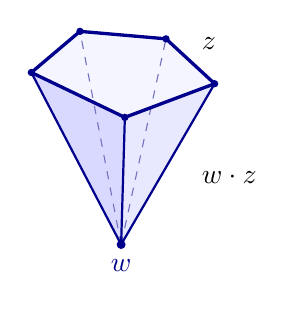
\begin{tikzpicture}[baseline=(current bounding box.center), scale=0.95]
    % Vértice del cono y vértices del ciclo z
    \coordinate (W)  at (0, 0);
    \coordinate (P1) at (-1.20, 2.30);
    \coordinate (P2) at (-0.55, 2.85);
    \coordinate (P3) at (0.60, 2.75);
    \coordinate (P4) at (1.25, 2.15);
    \coordinate (P5) at (0.05, 1.70);

    % Sombreado tridimensional del cono
    \fill[blue!4]  (P1) -- (P2) -- (P3) -- (P4) -- (P5) -- cycle;
    \fill[blue!15] (W) -- (P1) -- (P5) -- cycle;
    \fill[blue!9]  (W) -- (P5) -- (P4) -- cycle;

    % Aristas posteriores del cono
    \draw[dashed, blue!55!black!55] (W) -- (P2);
    \draw[dashed, blue!55!black!55] (W) -- (P3);

    % Aristas frontales del cono
    \draw[thick, blue!55!black] (W) -- (P1) (W) -- (P5) (W) -- (P4);

    % Ciclo afín z en la parte superior
    \draw[very thick, blue!55!black] (P1) -- (P2) -- (P3) -- (P4) -- (P5) -- cycle;

    % Vértices
    \foreach \P in {P1, P2, P3, P4, P5} {
        \fill[blue!55!black] (\P) circle (1.4pt);
    }
    \fill[blue!55!black] (W) circle (1.7pt) node[below=2pt] {$w$};

    % Etiquetas
    \node[above right] at (0.95, 2.48) {$z$};
    \node[right] at (0.95, 0.90) {$w \cdot z$};
\end{tikzpicture}
\]
En particular, como $z$ es un ciclo ($\partial_q(z) = 0$), concluimos que
\[
\partial_{q+1}(w \cdot z) = z.
\]
\end{dem}

\begin{teorema}
Sean $f, g \colon (X, A) \to (Y, B)$ funciones continuas tales que $f \simeq g$. Entonces
\[
f_* = g_* \colon H_q(X, A; R) \longrightarrow H_q(Y, B; R).
\]
\end{teorema}



%%%% Clase 36 del 02/11/26 inciada el 22/11/26 terminada el 22/11/2026

%%%%%% Clase 37 del 04/11/2026 iniciada el 22/11/2026


\begin{dem}
Haremos la prueba para el caso absoluto $f, g \colon X \to Y$, pues el mismo argumento se extiende al caso de parejas.

Como $f \simeq g$, existe una homotopía $H \colon X \times I \to Y$ tal que $H(x, 0) = f(x)$ y $H(x, 1) = g(x)$ para todo $x \in X$. Definamos las inclusiones $\lambda^0, \lambda^1 \colon X \to X \times I$ dadas por
\[
\lambda^0(x) = (x, 0) \quad \text{y} \quad \lambda^1(x) = (x, 1),
\]
de modo que $H \circ \lambda^0 = f$ y $H \circ \lambda^1 = g$. Aplicando homología, obtenemos
\[
(H \circ \lambda^0)_* = f_* \quad \text{y} \quad (H \circ \lambda^1)_* = g_*,
\]
lo cual implica
\[
H_* \circ \lambda^0_* = f_* \quad \text{y} \quad H_* \circ \lambda^1_* = g_*.
\]
Por lo tanto, basta demostrar que $\lambda^0_* = \lambda^1_*$.

Para ello, dado cualquier ciclo $[z] \in H_q(X; R)$, queremos ver que $\lambda^1_*([z]) = \lambda^0_*([z])$, es decir, $[\lambda^1_\#(z)] = [\lambda^0_\#(z)]$, o equivalentemente,
\[
[\lambda^1_\#(z) - \lambda^0_\#(z)] = 0 \in H_q(X \times I; R).
\]
Consideremos el siguiente diagrama entre los complejos de cadenas singulares de $X$ y $X \times I$:
\[
\begin{tikzcd}[column sep=2.6em, row sep=3.2em]
\cdots \arrow[r] &[-1em] S_{q+1}(X) \arrow[r, "\partial_{q+1}"] \arrow[d, shift right=0.55ex, "\lambda^0_\#"'] \arrow[d, shift left=0.55ex, "\lambda^1_\#"] & S_q(X) \arrow[r, "\partial_q"] \arrow[d, shift right=0.55ex, "\lambda^0_\#"'] \arrow[d, shift left=0.55ex, "\lambda^1_\#"] \arrow[dl, dashed, blue!55!black, "T_q^X"{description}] & S_{q-1}(X) \arrow[r] \arrow[d, shift right=0.55ex, "\lambda^0_\#"'] \arrow[d, shift left=0.55ex, "\lambda^1_\#"] \arrow[dl, dashed, blue!55!black, "T_{q-1}^X"{description}] &[-1em] \cdots \\
\cdots \arrow[r] & S_{q+1}(X \times I) \arrow[r, "\partial'_{q+1}"'] & S_q(X \times I) \arrow[r, "\partial'_q"'] & S_{q-1}(X \times I) \arrow[r] & \cdots
\end{tikzcd}
\]
A cada cadena $c \in S_q(X)$ le queremos asociar una $(q+1)$-cadena $T_q^X(c) \in S_{q+1}(X \times I)$, construyendo los homomorfismos $T_q^X \colon S_q(X) \to S_{q+1}(X \times I)$ por recursión de manera que satisfagan
\begin{equation}
\label{eq:homotopia_de_cadena}
\lambda^1_\#(c) - \lambda^0_\#(c) = \partial'_{q+1} T_q^X(c) + T_{q-1}^X \partial_q(c).
\end{equation}
Notemos que el segundo sumando no altera lo que buscamos, pues al evaluar \ref{eq:homotopia_de_cadena} en un ciclo $z \in Z_q(X)$ se tiene $\partial_q(z) = 0$, de donde
\[
\lambda^1_\#(z) - \lambda^0_\#(z) = \partial'_{q+1}(T_q^X(z)) \in B_q(X \times I),
\]
y por consiguiente $[\lambda^1_\#(z) - \lambda^0_\#(z)] = 0 \in H_q(X \times I; R)$.

\begin{definicion}
     A una familia de homomorfismos $\{T_q^X\}$ que satisface la igualdad $\ref{eq:homotopia_de_cadena}$ se le llama una \textit{homotopía de cadenas} (entre $\lambda^0_\#$ y $\lambda^1_\#$). Para llevar a cabo la construcción recursiva de esta homotopía de cadenas, pediremos además que sea natural.
\end{definicion}

Recordemos que una \textit{transformación natural} $T \colon F \Rightarrow G$ entre dos funtores $F, G \colon \mathcal{C} \to \mathcal{D}$ asigna a cada objeto $X \in \operatorname{Obj}(\mathcal{C})$ un morfismo compatible con los morfismos de $\mathcal{C}$. En nuestro caso, consideramos $\mathcal{C} = \Top$ y $\mathcal{D} = \text{C.C.\ } R\text{-Mod}$ (la categoría de complejos de cadenas de $R$-módulos), junto con los funtores $F$ y $G$ dados en cada grado $q$ sobre los objetos por
\[
F(X)_q = S_q(X), \qquad G(X)_q = S_{q+1}(X \times I),
\]
y sobre cada función continua $f \colon X \to Y$ por los homomorfismos inducidos
\[
F(f)_q = f_\# \colon S_q(X) \longrightarrow S_q(Y), \qquad G(f)_q = (f \times \operatorname{Id}_I)_\# \colon S_{q+1}(X \times I) \longrightarrow S_{q+1}(Y \times I).
\]

Pedir que la familia de homomorfismos $T_q^X \colon S_q(X) \to S_{q+1}(X \times I)$ (para cada $X \in \operatorname{Obj}(\Top)$) sea natural en cada grado $q$ significa que, dada cualquier función continua $f \colon Z \to X$, conmuta el siguiente diagrama:
\[
\begin{tikzcd}[column sep=3.4em, row sep=2.6em]
F(Z)_q = S_q(Z) \arrow[r, "T_q^Z"] \arrow[d, "f_\#"'] & G(Z)_q = S_{q+1}(Z \times I) \arrow[d, "(f \times \operatorname{Id}_I)_\#"] \\
F(X)_q = S_q(X) \arrow[r, "T_q^X"'] & G(X)_q = S_{q+1}(X \times I)
\end{tikzcd}
\]

Como $S_q(X)$ es el $R$-módulo libre generado por los $q$-simplejos singulares $\sigma \colon \Delta^q \to X$, para definir $T_q^X$ basta determinar su valor en cada generador $\sigma$. Tomando en el diagrama anterior $Z = \Delta^q$ y $f = \sigma \colon \Delta^q \to X$, y denotando por
\[
P_q \equiv T_q^{\Delta^q}(\operatorname{Id}_{\Delta^q}) \in S_{q+1}(\Delta^q \times I),
\]
obtenemos el diagrama conmutativo y el seguimiento de la identidad $\operatorname{Id}_{\Delta^q} \in S_q(\Delta^q)$:
\[
\begin{tikzcd}[column sep=2.8em, row sep=2.6em]
S_q(\Delta^q) \arrow[r, "T_q^{\Delta^q}"] \arrow[d, "\sigma_\#"'] & S_{q+1}(\Delta^q \times I) \arrow[d, "(\sigma \times \operatorname{Id}_I)_\#"] \\
S_q(X) \arrow[r, "T_q^X"'] & S_{q+1}(X \times I)
\end{tikzcd}
\hspace{2em}
\begin{tikzcd}[column sep=2.2em, row sep=2.6em]
\operatorname{Id}_{\Delta^q} \arrow[r, mapsto] \arrow[d, mapsto] & P_q \arrow[d, mapsto] \\
\sigma \arrow[r, mapsto] & T_q^X(\sigma)
\end{tikzcd}
\]
Puesto que $\sigma_\#(\operatorname{Id}_{\Delta^q}) = \sigma \circ \operatorname{Id}_{\Delta^q} = \sigma$, la conmutatividad del diagrama fuerza la igualdad
\[
{T_q^X(\sigma) = T_q^X(\sigma_\#(\operatorname{Id}_{\Delta^q})) = (\sigma \times \operatorname{Id}_I)_\#(T_q^{\Delta^q}(\operatorname{Id}_{\Delta^q})) = (\sigma \times \operatorname{Id}_I)_\#(P_q).}
\]
De este modo, construir toda la familia natural $\{T_q^X\}$ para cualquier espacio $X$ se reduce a elegir, para cada $q \geq 0$, una única $(q+1)$-cadena universal $P_q \in S_{q+1}(\Delta^q \times I)$.
Para determinar la condición que debe cumplir cada $P_q \in S_{q+1}(\Delta^q \times I)$, apliquemos primero la naturalidad en grado $q-1$ a cada inclusión de cara $F_q^i \colon \Delta^{q-1} \to \Delta^q$ ($0 \leq i \leq q$). Obtenemos el siguiente diagrama conmutativo junto con el recorrido de $\operatorname{Id}_{\Delta^{q-1}} \in S_{q-1}(\Delta^{q-1})$:
\[
\begin{tikzcd}[column sep=3.2em, row sep=2.6em]
S_{q-1}(\Delta^{q-1}) \arrow[r, "T_{q-1}^{\Delta^{q-1}}"] \arrow[d, "(F_q^i)_\#"'] & S_q(\Delta^{q-1} \times I) \arrow[d, "(F_q^i \times \operatorname{Id}_I)_\#"] \\
S_{q-1}(\Delta^q) \arrow[r, "T_{q-1}^{\Delta^q}"'] & S_q(\Delta^q \times I)
\end{tikzcd}
\hspace{1.8em}
\begin{tikzcd}[column sep=2.2em, row sep=2.6em]
\operatorname{Id}_{\Delta^{q-1}} \arrow[r, mapsto] \arrow[d, mapsto] & P_{q-1} \arrow[d, mapsto] \\
F_q^i \arrow[r, mapsto] & T_{q-1}^{\Delta^q}(F_q^i)
\end{tikzcd}
\]
Como $(F_q^i)_\#(\operatorname{Id}_{\Delta^{q-1}}) = F_q^i$, la conmutatividad del diagrama nos da
\begin{align*}
T_{q-1}^{\Delta^q}(F_q^i) &= T_{q-1}^{\Delta^q}\!\left((F_q^i)_\#(\operatorname{Id}_{\Delta^{q-1}})\right) \\
&= (F_q^i \times \operatorname{Id}_I)_\#\!\left(T_{q-1}^{\Delta^{q-1}}(\operatorname{Id}_{\Delta^{q-1}})\right) \\
&= (F_q^i \times \operatorname{Id}_I)_\#(P_{q-1}),
\end{align*}
donde $P_{q-1} \equiv T_{q-1}^{\Delta^{q-1}}(\operatorname{Id}_{\Delta^{q-1}})$.

Evaluando ahora la identidad de homotopía de cadenas $(\dagger)$ en el espacio $X = \Delta^q$ sobre el $q$-simplejo $\operatorname{Id}_{\Delta^q} \in S_q(\Delta^q)$, y usando que $(\lambda^k_{\Delta^q})_\#(\operatorname{Id}_{\Delta^q}) = \lambda^k_{\Delta^q}$ (para $k = 0, 1$) junto con $\partial_q(\operatorname{Id}_{\Delta^q}) = \sum_{i=0}^q (-1)^i F_q^i$, obtenemos
\[
\lambda^1_{\Delta^q} - \lambda^0_{\Delta^q} = \partial_{q+1}(P_q) + \sum_{i=0}^q (-1)^i (F_q^i \times \operatorname{Id}_I)_\#(P_{q-1}).
\]
Despejando $\partial_{q+1}(P_q)$, resulta la condición recursiva
\[
\partial_{q+1}(P_q) = \lambda^1_{\Delta^q} - \lambda^0_{\Delta^q} - \sum_{i=0}^q (-1)^i (F_q^i \times \operatorname{Id}_I)_\#(P_{q-1}).
\]
Llevaremos a cabo la definición recursiva de $P_q$ utilizando cadenas afines en el conjunto convexo $\Delta^q \times I$ y el lema anterior sobre la frontera del cono de un ciclo afín.

Para cada $q \geq 0$, sea
\[
b_q = \left(\frac{1}{q+1}, \dots, \frac{1}{q+1}\right)
\]
el baricentro de $\Delta^q$, y consideremos el punto central del prisma
\[
p_q = \left(b_q, \frac{1}{2}\right) \in \Delta^q \times I.
\]

Empezamos con el caso base $q = 0$, para el cual buscamos una $1$-cadena afín $P_0 \in S_1(\Delta^0 \times I)$. Identificando $\Delta^0 = \{e_0\}$, tenemos los $0$-simplejos afines $\lambda_{\Delta^0}^0 = \langle\!\langle (e_0, 0) \rangle\!\rangle$ y $\lambda_{\Delta^0}^1 = \langle\!\langle (e_0, 1) \rangle\!\rangle$. Definimos
\[
P_0 \equiv p_0 \cdot (\lambda_{\Delta^0}^1 - \lambda_{\Delta^0}^0).
\]
\[
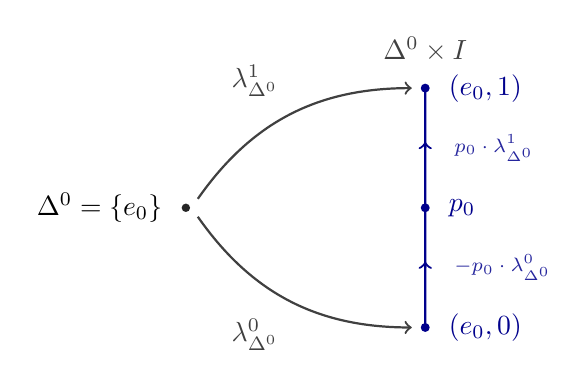
\begin{tikzpicture}[baseline=(current bounding box.center), scale=0.95]
    % Espacio \Delta^0 a la izquierda
    \coordinate (D) at (0, 1.6);
    \fill[black!85] (D) circle (1.6pt);
    \node[left=5pt] at (D) {$\Delta^0 = \{e_0\}$};

    % Segmento vertical \Delta^0 \times I a la derecha
    \coordinate (B) at (3.2, 0.0);
    \coordinate (M) at (3.2, 1.6);
    \coordinate (T) at (3.2, 3.2);

    \node[above=6pt, black!75] at (T) {$\Delta^0 \times I$};

    % Subsegmentos orientados que conforman P_0
    \draw[->, thick, blue!55!black] (B) -- (3.2, 0.88);
    \draw[thick, blue!55!black] (3.2, 0.80) -- (M);
    \draw[->, thick, blue!55!black] (M) -- (3.2, 2.48);
    \draw[thick, blue!55!black] (3.2, 2.40) -- (T);

    % Flechas curvas de las inclusiones \lambda_{\Delta^0}^1 y \lambda_{\Delta^0}^0
    \draw[->, thick, black!75] (0.16, 1.72) to[out=55, in=180]
        node[above left=2pt, pos=0.52] {$\lambda_{\Delta^0}^1$} (3.02, 3.2);
    \draw[->, thick, black!75] (0.16, 1.48) to[out=-55, in=180]
        node[below left=2pt, pos=0.52] {$\lambda_{\Delta^0}^0$} (3.02, 0.0);

    % Puntos distinguidos en \Delta^0 \times I
    \fill[blue!55!black] (T) circle (1.7pt) node[right=5pt] {$(e_0, 1)$};
    \fill[blue!55!black] (M) circle (1.7pt) node[right=5pt] {$p_0$};
    \fill[blue!55!black] (B) circle (1.7pt) node[right=5pt] {$(e_0, 0)$};

    % Etiquetas de las 1-cadenas orientadas
    \node[right=7pt, blue!55!black!85] at (3.2, 2.4) {\scriptsize $p_0 \cdot \lambda_{\Delta^0}^1$};
    \node[right=7pt, blue!55!black!85] at (3.2, 0.8) {\scriptsize $-p_0 \cdot \lambda_{\Delta^0}^0$};
\end{tikzpicture}
\]
Como $\lambda_{\Delta^0}^1 - \lambda_{\Delta^0}^0$ es una $0$-cadena (por lo tanto un $0$-ciclo, y con suma de coeficientes igual a cero), se cumple $\partial_1(P_0) = \lambda_{\Delta^0}^1 - \lambda_{\Delta^0}^0$. En forma explícita:
\begin{align*}
\partial_1(P_0) &= \partial_1(p_0 \cdot \lambda_{\Delta^0}^1 - p_0 \cdot \lambda_{\Delta^0}^0) \\
&= \partial_1(p_0 \cdot \lambda_{\Delta^0}^1) - \partial_1(p_0 \cdot \lambda_{\Delta^0}^0) \\
&= \bigl(\langle\!\langle (e_0, 1) \rangle\!\rangle - \langle\!\langle p_0 \rangle\!\rangle\bigr) - \bigl(\langle\!\langle (e_0, 0) \rangle\!\rangle - \langle\!\langle p_0 \rangle\!\rangle\bigr) \\
&= \lambda_{\Delta^0}^1 - \lambda_{\Delta^0}^0.
\end{align*}

Por recursión, para cada $q \geq 1$ definimos la $(q+1)$-cadena afín $P_q \in S_{q+1}(\Delta^q \times I)$ mediante
\[
P_q = p_q \cdot \bigg(\lambda_{\Delta^q}^1 - \lambda_{\Delta^q}^0 - \sum_{i=0}^q (-1)^i (F_q^i \times \operatorname{Id}_I)_\#(P_{q-1})\bigg).
\]
Denotando por
\[
z_q = \lambda_{\Delta^q}^1 - \lambda_{\Delta^q}^0 - \sum_{i=0}^q (-1)^i (F_q^i \times \operatorname{Id}_I)_\#(P_{q-1}),
\]
\begin{nota}
Se prueba por inducción sobre $q$ que la $q$-cadena afín $z_q$ definida arriba es efectivamente un ciclo, lo cual permite aplicar el lema de la construcción cono en cada paso de la recursión.
\end{nota}



\begin{ejemplo}
Para $q = 1$, la fórmula recursiva da la $2$-cadena afín
\[
P_1 = p_1 \cdot \Bigl(\lambda_{\Delta^1}^1 - \lambda_{\Delta^1}^0 - (F_1^0 \times \operatorname{Id}_I)_\#(P_0) + (F_1^1 \times \operatorname{Id}_I)_\#(P_0)\Bigr),
\]
que triangula el cuadrado $\Delta^1 \times I$ en seis $2$-simplejos afines con vértice común en $p_1$. Geométricamente, las cadenas $P_0$, $P_1$ y $P_2$ se visualizan como sigue:
\[
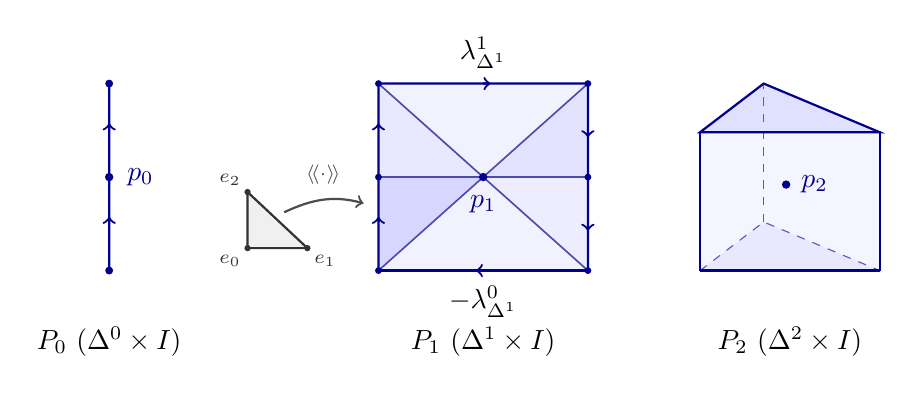
\begin{tikzpicture}[baseline=(current bounding box.center), scale=0.95]
    % === P_0 en \Delta^0 x I ===
    \coordinate (B0) at (0.4, 0.0);
    \coordinate (M0) at (0.4, 1.25);
    \coordinate (T0) at (0.4, 2.5);

    \draw[->, thick, blue!55!black] (B0) -- (0.4, 0.72);
    \draw[thick, blue!55!black] (0.4, 0.65) -- (M0);
    \draw[->, thick, blue!55!black] (M0) -- (0.4, 1.97);
    \draw[thick, blue!55!black] (0.4, 1.90) -- (T0);

    \fill[blue!55!black] (B0) circle (1.5pt);
    \fill[blue!55!black] (M0) circle (1.6pt) node[right=3pt] {$p_0$};
    \fill[blue!55!black] (T0) circle (1.5pt);

    \node at (0.4, -0.95) {$P_0$ ($\Delta^0 \times I$)};

    % === Pequeño \Delta^2 indicando un 2-simplejo afín en P_1 ===
    \coordinate (D0) at (2.25, 0.30);
    \coordinate (D1) at (3.05, 0.30);
    \coordinate (D2) at (2.25, 1.05);

    \fill[gray!12] (D0) -- (D1) -- (D2) -- cycle;
    \draw[thick, black!80] (D0) -- (D1) -- (D2) -- cycle;
    \fill[black!80] (D0) circle (1.2pt) node[below left=-1pt] {\scriptsize $e_0$};
    \fill[black!80] (D1) circle (1.2pt) node[below right=-1pt] {\scriptsize $e_1$};
    \fill[black!80] (D2) circle (1.2pt) node[above left=-1pt] {\scriptsize $e_2$};

    \draw[->, thick, black!70] (2.74, 0.78) to[out=25, in=165]
        node[midway, above=2pt] {\scriptsize $\langle\!\langle \cdot \rangle\!\rangle$} (3.80, 0.90);

    % === P_1 en \Delta^1 x I ===
    \coordinate (BL) at (4.0, 0.0);
    \coordinate (BR) at (6.8, 0.0);
    \coordinate (TR) at (6.8, 2.5);
    \coordinate (TL) at (4.0, 2.5);
    \coordinate (ML) at (4.0, 1.25);
    \coordinate (MR) at (6.8, 1.25);
    \coordinate (P1) at (5.4, 1.25);

    % Sombreado suave de los seis 2-simplejos
    \fill[blue!16] (P1) -- (BL) -- (ML) -- cycle;
    \fill[blue!9]  (P1) -- (ML) -- (TL) -- cycle;
    \fill[blue!5]  (P1) -- (TL) -- (TR) -- cycle;
    \fill[blue!11] (P1) -- (TR) -- (MR) -- cycle;
    \fill[blue!7]  (P1) -- (MR) -- (BR) -- cycle;
    \fill[blue!5]  (P1) -- (BR) -- (BL) -- cycle;

    % Rayos interiores desde p_1
    \foreach \V in {BL, BR, TR, TL, ML, MR} {
        \draw[semithick, blue!55!black!70] (P1) -- (\V);
    }

    % Frontera orientada de \Delta^1 x I
    % Superior: +\lambda_{\Delta^1}^1 (hacia la derecha)
    \draw[->, thick, blue!55!black] (TL) -- (5.50, 2.5);
    \draw[thick, blue!55!black] (5.40, 2.5) -- (TR);
    \node[above=2pt] at (5.4, 2.5) {$\lambda_{\Delta^1}^1$};

    % Inferior: -\lambda_{\Delta^1}^0 (hacia la izquierda)
    \draw[->, thick, blue!55!black] (BR) -- (5.30, 0.0);
    \draw[thick, blue!55!black] (5.40, 0.0) -- (BL);
    \node[below=2pt] at (5.4, 0.0) {$-\lambda_{\Delta^1}^0$};

    % Izquierda: +(F_1^1 x Id_I)_#(P_0) (hacia arriba)
    \draw[->, thick, blue!55!black] (BL) -- (4.0, 0.72);
    \draw[thick, blue!55!black] (4.0, 0.65) -- (ML);
    \draw[->, thick, blue!55!black] (ML) -- (4.0, 1.97);
    \draw[thick, blue!55!black] (4.0, 1.90) -- (TL);

    % Derecha: -(F_1^0 x Id_I)_#(P_0) (hacia abajo)
    \draw[->, thick, blue!55!black] (TR) -- (6.8, 1.78);
    \draw[thick, blue!55!black] (6.8, 1.85) -- (MR);
    \draw[->, thick, blue!55!black] (MR) -- (6.8, 0.53);
    \draw[thick, blue!55!black] (6.8, 0.60) -- (BR);

    % Vértices y baricentro p_1
    \foreach \V in {BL, BR, TR, TL, ML, MR} {
        \fill[blue!55!black] (\V) circle (1.3pt);
    }
    \fill[blue!55!black] (P1) circle (1.6pt) node[below=3pt] {$p_1$};

    \node at (5.4, -0.95) {$P_1$ ($\Delta^1 \times I$)};

    % === P_2 en \Delta^2 x I ===
    \coordinate (A0) at (8.30, 0.00);
    \coordinate (A1) at (10.70, 0.00);
    \coordinate (A2) at (9.15, 0.65);
    \coordinate (B0) at (8.30, 1.85);
    \coordinate (B1) at (10.70, 1.85);
    \coordinate (B2) at (9.15, 2.50);
    \coordinate (P2) at (9.45, 1.15);

    % Sombreado del prisma (cara frontal, base y tapa superior)
    \fill[blue!4]  (A0) -- (A1) -- (B1) -- (B0) -- cycle;
    \fill[blue!9]  (A0) -- (A1) -- (A2) -- cycle;
    \fill[blue!12] (B0) -- (B1) -- (B2) -- cycle;

    % Aristas ocultas del prisma (solo las 3 aristas traseras)
    \draw[dashed, blue!55!black!65] (A0) -- (A2) -- (A1);
    \draw[dashed, blue!55!black!65] (A2) -- (B2);

    % Aristas visibles del prisma
    \draw[thick, blue!55!black] (A0) -- (A1);
    \draw[thick, blue!55!black] (A0) -- (B0) (A1) -- (B1);
    \draw[thick, blue!55!black] (B0) -- (B1) -- (B2) -- cycle;

    % Baricentro p_2 en el interior
    \fill[blue!55!black] (P2) circle (1.6pt) node[right=2pt] {$p_2$};

    \node at (9.50, -0.95) {$P_2$ ($\Delta^2 \times I$)};
\end{tikzpicture}
\]
\end{ejemplo}
%%%% Clase 37 del 04/11/26 inciada el 22/11/26 terminada el 22/11/2026

%%%%%% Clase 38 del 06/11/2026 iniciada el 22/11/2026
Vimos que si tenemos una homotopía de cadenas natural $T$, entonces quedan determinadas las cadenas universales $P_q$. Ahora falta verificar el recíproco: que a partir de las cadenas $P_q$ construidas podemos definir la homotopía de cadenas natural $T$.

\begin{definicion}
Dado un espacio topológico $X$, definimos el homomorfismo $T_q^X \colon S_q(X) \to S_{q+1}(X \times I)$ sobre cada $q$-simplejo singular $\sigma \colon \Delta^q \to X$ como
\[
T_q^X(\sigma) = (\sigma \times \operatorname{Id}_I)_\#(P_q),
\]
donde $P_q \in S_{q+1}(\Delta^q \times I)$, y lo extendemos por linealidad a todo $S_q(X)$.
\end{definicion}

\begin{ejercicio}
    % ID: 74
Ver que la familia $T = \{T_q^X\}$ así definida es natural.
\end{ejercicio}

{Afirmación:} Para las inclusiones $\lambda^i \colon X \hookrightarrow X \times I$ ($i = 0, 1$), se cumple
\[
\lambda^1_\# - \lambda^0_\# = \partial_{q+1} \circ T_q^X + T_{q-1}^X \circ \partial_q.
\]

Basta verificar la igualdad sobre cada generador $\sigma \colon \Delta^q \to X$. Observemos primero que claramente
\[
(\sigma \times \operatorname{Id}_I) \circ \lambda^i_{\Delta^q} = \lambda^i \circ \sigma \qquad (i = 0, 1).
\]
Ahora, evaluando el lado derecho en $\sigma$, obtenemos
\begin{align*}
(\partial_{q+1} \circ T_q^X + T_{q-1}^X \circ \partial_q)(\sigma)
&= \partial_{q+1}(T_q^X(\sigma)) + T_{q-1}^X(\partial_q(\sigma)) \\
&= \partial_{q+1}\!\left((\sigma \times \operatorname{Id}_I)_\#(P_q)\right) + T_{q-1}^X\!\left(\sum_{i=0}^q (-1)^i \sigma \circ F_q^i\right) \\
&= (\sigma \times \operatorname{Id}_I)_\#(\partial_{q+1}(P_q)) + \sum_{i=0}^q (-1)^i T_{q-1}^X(\sigma \circ F_q^i).
\end{align*}
Por otro lado, claramente se cumple que
\begin{equation}
\tag{1}
(\sigma \circ F_q^i) \times \operatorname{Id}_I = (\sigma \times \operatorname{Id}_I) \circ (F_q^i \times \operatorname{Id}_I).
\end{equation}
Además, por la construcción recursiva de $P_q$ sabemos que
\[
\partial_{q+1}(P_q) = \lambda^1_{\Delta^q} - \lambda^0_{\Delta^q} - \sum_{i=0}^q (-1)^i (F_q^i \times \operatorname{Id}_I)_\#(P_{q-1}),
\]
y por la definición de $T_{q-1}^X$ junto con $(1)$,
\begin{align*}
T_{q-1}^X(\sigma \circ F_q^i) &= ((\sigma \circ F_q^i) \times \operatorname{Id}_I)_\#(P_{q-1}) \\
&\stackrel{(1)}{=} (\sigma \times \operatorname{Id}_I)_\# \circ (F_q^i \times \operatorname{Id}_I)_\#(P_{q-1}).
\end{align*}

Sustituyendo estas identidades en el desarrollo anterior y factorizando $(\sigma \times \operatorname{Id}_I)_\#$ por linealidad, obtenemos
\begin{align*}
(\partial_{q+1} \circ T_q^X + T_{q-1}^X \circ \partial_q)(\sigma)
&= (\sigma \times \operatorname{Id}_I)_\#\!\left(\lambda^1_{\Delta^q} - \lambda^0_{\Delta^q} - \sum_{i=0}^q (-1)^i (F_q^i \times \operatorname{Id}_I)_\#(P_{q-1})\right) \\
&\quad + (\sigma \times \operatorname{Id}_I)_\#\!\left(\sum_{i=0}^q (-1)^i (F_q^i \times \operatorname{Id}_I)_\#(P_{q-1})\right) \\
&= (\sigma \times \operatorname{Id}_I)_\#(\lambda^1_{\Delta^q} - \lambda^0_{\Delta^q}) \\
&= (\sigma \times \operatorname{Id}_I) \circ \lambda^1_{\Delta^q} - (\sigma \times \operatorname{Id}_I) \circ \lambda^0_{\Delta^q} \\
&= \lambda^1 \circ \sigma - \lambda^0 \circ \sigma \\
&= \lambda^1_\#(\sigma) - \lambda^0_\#(\sigma),
\end{align*}
donde en la penúltima igualdad utilizamos que $(\sigma \times \operatorname{Id}_I) \circ \lambda^i_{\Delta^q} = \lambda^i \circ \sigma$. Esto concluye la demostración de la afirmación.

Con ello queda construida la homotopía de cadenas $\{T_q^X\}$ entre $\lambda^0_\#$ y $\lambda^1_\#$, de donde $\lambda^0_* = \lambda^1_*$ y, por consiguiente, $f_* = g_*$.
\end{dem}
\begin{nota}
Para parejas de espacios y funciones continuas $f, g \colon (X, A) \to (Y, B)$, por la naturalidad de $T$ tenemos el diagrama conmutativo
\[
\begin{tikzcd}[column sep=2.8em, row sep=2.4em]
S_q(X) \arrow[r, "T_q^X"] & S_{q+1}(X \times I) \\
S_q(A) \arrow[u, hook, "i_\#"] \arrow[r, "T_q^A"'] & S_{q+1}(A \times I) \arrow[u, hook, "(i \times \operatorname{Id}_I)_\#"']
\end{tikzcd}
\]
En consecuencia, $T_q^X$ induce un homomorfismo en los cocientes:
\[
\begin{tikzcd}[column sep=3.0em, row sep=1.4em]
S_q(X)/S_q(A) \arrow[r, "\overline{T}_q^X"] \arrow[d, phantom, "\equiv"{description, sloped, inner sep=1pt}] & S_{q+1}(X \times I)/S_{q+1}(A \times I) \arrow[d, phantom, "\equiv"{description, sloped, inner sep=1pt}] \\
S_q(X, A) \arrow[r, "T_q^{(X, A)}"'] & S_{q+1}(X \times I, A \times I)
\end{tikzcd}
\]
donde $T_q^{(X, A)}$ es una homotopía de cadenas entre $(\lambda^1_{(X, A)})_\#$ y $(\lambda^0_{(X, A)})_\#$, para las inclusiones
\[
\lambda^i_{(X, A)} \colon (X, A) \hookrightarrow (X \times I, A \times I) \qquad (i = 0, 1).
\]
\end{nota}

\begin{definicion}
Sean $\varphi, \psi \colon (C_*, \partial_*^C) \to (D_*, \partial_*^D)$ morfismos de complejos de cadenas de $R$-módulos. Decimos que $\varphi$ es \textit{homotópico de cadenas} a $\psi$, y escribimos $\varphi \underset{c}{\simeq} \psi$, si existen homomorfismos de $R$-módulos $T_q \colon C_q \to D_{q+1}$ tales que, para todo $q$,
\[
\varphi_q - \psi_q = \partial_{q+1}^D \circ T_q + T_{q-1} \circ \partial_q^C.
\]
En tal caso, se tiene que $\varphi_* = \psi_* \colon H_*(C_*, \partial_*^C) \to H_*(D_*, \partial_*^D)$.
\end{definicion}
\begin{ejercicio}
    % ID: 75
Sean
\[
\begin{tikzcd}[column sep=2.6em]
(C_*, \partial_*^C) \arrow[r, shift left=0.6ex, "\varphi"] \arrow[r, shift right=0.6ex, "\psi"'] & (D_*, \partial_*^D) \arrow[r, "\beta"] & (E_*, \partial_*^E)
\end{tikzcd}
\]
morfismos de complejos de cadenas tales que $\varphi \underset{c}{\simeq} \psi$. Ver que $\beta \circ \varphi \underset{c}{\simeq} \beta \circ \psi$.
\end{ejercicio}

\begin{coro}
Sean $f, g \colon X \to Y$ funciones continuas tales que $f \simeq g$. Entonces $f_\# \underset{c}{\simeq} g_\#$ y, en particular,
\[
f_* = g_* \colon H_*(X; R) \longrightarrow H_*(Y; R).
\]
\end{coro}

\begin{dem}
Sea $H \colon X \times I \to Y$ una homotopía entre $f$ y $g$. Como $\lambda^0_\# \underset{c}{\simeq} \lambda^1_\#$, por el ejercicio anterior aplicado a $\beta = H_\#$ obtenemos
\begin{align*}
f_\# = (H \circ \lambda^0)_\# &= H_\# \circ \lambda^0_\# \\
&\underset{c}{\simeq} H_\# \circ \lambda^1_\# = (H \circ \lambda^1)_\# = g_\#,
\end{align*}
de donde $f_\# \underset{c}{\simeq} g_\#$, y por consiguiente $f_* = g_*$.
\end{dem}

\begin{coro}
Supongamos que $X \simeq Y$. Entonces $H_q(X; R) \cong H_q(Y; R)$ para todo $q$.
\end{coro}

\begin{dem}
Como $X \simeq Y$, existen funciones continuas $X \xrightarrow{f} Y \xrightarrow{g} X$ tales que $g \circ f \simeq \operatorname{Id}_X$ y $f \circ g \simeq \operatorname{Id}_Y$. Por el teorema de invariancia homotópica,
\[
g_* \circ f_* = (g \circ f)_* = (\operatorname{Id}_X)_* = \operatorname{Id}_{H_q(X; R)}
\quad \text{y} \quad
f_* \circ g_* = (f \circ g)_* = (\operatorname{Id}_Y)_* = \operatorname{Id}_{H_q(Y; R)}.
\]
Por lo tanto, $f_* \colon H_q(X; R) \to H_q(Y; R)$ es un isomorfismo para todo $q$.
\end{dem}

\begin{definicion}[Escisión]
Sea $(X, A)$ una pareja de espacios topológicos, sea $U \subset A$ y consideremos la inclusión
\[
j \colon (X - U, A - U) \hookrightarrow (X, A).
\]
Decimos que $j$ es una \textit{escisión} si el homomorfismo inducido en homología
\[
j_* \colon H_q(X - U, A - U; R) \xrightarrow{\;\cong\;} H_q(X, A; R)
\]
es un isomorfismo para todo $q$.
\end{definicion}

Nuestro objetivo será determinar bajo qué condiciones sobre $U$ la inclusión $j$ resulta ser una escisión.

\begin{ejemplo}
Supongamos que $X$ es convexo, $U \subset A \subset X$, y consideremos el caso $q = 1$:
\[
H_1(X - U, A - U; R) \xrightarrow{\;j_*\;} H_1(X, A; R) \ni [c].
\]
¿Cómo vemos que $j_*$ es suprayectivo?
\[
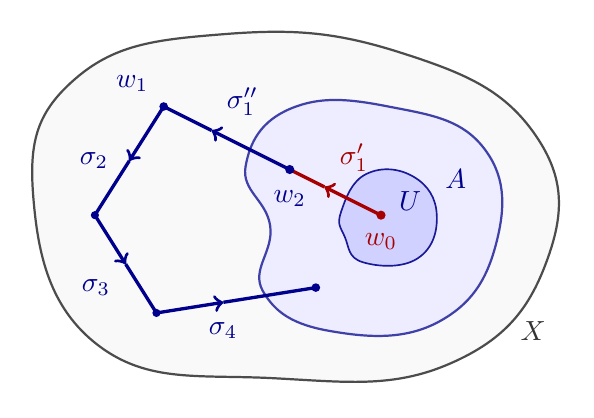
\begin{tikzpicture}[baseline=(current bounding box.center), scale=0.92]
    % === Regiones orgánicas anidadas U \subset A \subset X ===
    % Espacio convexo X (contorno general suave)
    \draw[thick, black!70, fill=gray!5] plot[smooth cycle, tension=0.75] coordinates {
        (-3.15,  0.30)
        (-2.55,  1.95)
        (-0.50,  2.55)
        ( 1.90,  2.30)
        ( 3.75,  1.20)
        ( 3.95, -0.55)
        ( 2.60, -2.00)
        ( 0.15, -2.20)
        (-2.25, -1.75)
    };

    % Subespacio A \subset X (región general)
    \draw[thick, blue!55!black!75, fill=blue!7] plot[smooth cycle, tension=0.75] coordinates {
        (-0.22,  0.72)
        ( 0.40,  1.52)
        ( 1.75,  1.55)
        ( 3.05,  1.00)
        ( 3.25, -0.30)
        ( 2.45, -1.42)
        ( 0.95, -1.55)
        ( 0.02, -1.00)
        ( 0.12, -0.10)
    };

    % Subconjunto U \subset A (región general)
    \draw[semithick, blue!55!black!90, fill=blue!18] plot[smooth cycle, tension=0.75] coordinates {
        ( 1.10,  0.10)
        ( 1.45,  0.62)
        ( 2.10,  0.58)
        ( 2.42,  0.05)
        ( 2.15, -0.55)
        ( 1.40, -0.60)
        ( 1.15, -0.25)
    };

    % Etiquetas de las regiones
    \node[black!80]      at (3.75, -1.55) {$X$};
    \node[blue!55!black] at (2.68,  0.55) {$A$};
    \node[blue!55!black] at (2.05,  0.24) {$U$};

    % === Vértices del ciclo relativo c = \sigma_1 + \sigma_2 + \sigma_3 + \sigma_4 ===
    \coordinate (W0) at ( 1.65,  0.05);
    \coordinate (W2) at ( 0.39,  0.68);
    \coordinate (W1) at (-1.35,  1.55);
    \coordinate (V2) at (-2.30,  0.05);
    \coordinate (V3) at (-1.45, -1.30);
    \coordinate (V4) at ( 0.75, -0.95);

    % Subdivisión \sigma_1' = <<w_0, w_2>> (en A, entrando a U)
    \draw[->, very thick, red!65!black] (W0) -- (0.869, 0.4405);
    \draw[very thick, red!65!black] (0.869, 0.4405) -- (W2);
    \node[red!65!black, above right=2pt] at (0.87, 0.44) {$\sigma_1'$};

    % Subdivisión \sigma_1'' = <<w_2, w_1>> (en X - U)
    \draw[->, very thick, blue!55!black] (W2) -- (-0.689, 1.2195);
    \draw[very thick, blue!55!black] (-0.689, 1.2195) -- (W1);
    \node[blue!55!black, above right=2pt] at (-0.69, 1.22) {$\sigma_1''$};

    % Resto del ciclo relativo: \sigma_2, \sigma_3, \sigma_4 (en X - U)
    \draw[->, very thick, blue!55!black] (W1) -- (-1.825, 0.80);
    \draw[very thick, blue!55!black] (-1.825, 0.80) -- (V2);
    \node[blue!55!black, left=4pt] at (-1.83, 0.80) {$\sigma_2$};

    \draw[->, very thick, blue!55!black] (V2) -- (-1.875, -0.625);
    \draw[very thick, blue!55!black] (-1.875, -0.625) -- (V3);
    \node[blue!55!black, below left=2pt] at (-1.88, -0.63) {$\sigma_3$};

    \draw[->, very thick, blue!55!black] (V3) -- (-0.526, -1.153);
    \draw[very thick, blue!55!black] (-0.526, -1.153) -- (V4);
    \node[blue!55!black, below=4pt] at (-0.53, -1.15) {$\sigma_4$};

    % Puntos y etiquetas de los vértices
    \fill[red!65!black]  (W0) circle (1.8pt) node[below=3pt] {$w_0$};
    \fill[blue!55!black] (W2) circle (1.8pt) node[below=4pt] {$w_2$};
    \fill[blue!55!black] (W1) circle (1.7pt) node[above left=2pt] {$w_1$};
    \fill[blue!55!black] (V2) circle (1.6pt);
    \fill[blue!55!black] (V3) circle (1.6pt);
    \fill[blue!55!black] (V4) circle (1.7pt);
\end{tikzpicture}

\]
Sea $c = \sigma_1 + \sigma_2 + \sigma_3 + \sigma_4$ un $1$-ciclo relativo en $(X, A)$, donde $\sigma_1 = \langle\!\langle w_0, w_1 \rangle\!\rangle$ parte de $w_0 \in U$. Elegimos un punto intermedio $w_2 \in A - U$ sobre el segmento que une $w_0$ con $w_1$, y definimos los $1$-simplejos afines
\[
\sigma_1' = \langle\!\langle w_0, w_2 \rangle\!\rangle \in S_1(A)
\quad \text{y} \quad
\sigma_1'' = \langle\!\langle w_2, w_1 \rangle\!\rangle \in S_1(X - U).
\]
Consideremos ahora el ciclo relativo $\tilde{c} = \sigma_1'' + \sigma_2 + \sigma_3 + \sigma_4$ en $(X - U, A - U)$. Entonces
\[
\tilde{c} - c = \sigma_1'' - \sigma_1.
\]
Como $X$ es convexo, podemos tomar el $2$-simplejo afín $d = \langle\!\langle w_0, w_2, w_1 \rangle\!\rangle \in S_2(X)$, cuya frontera es
\[
\partial_2(d) = \langle\!\langle w_2, w_1 \rangle\!\rangle - \langle\!\langle w_0, w_1 \rangle\!\rangle + \langle\!\langle w_0, w_2 \rangle\!\rangle = \sigma_1'' - \sigma_1 + \sigma_1'.
\]
En consecuencia,
\[
\tilde{c} - c = \partial_2(d) - \sigma_1' \in B_1(X, A),
\]
por lo que $[\tilde{c}] = [c] \in H_1(X, A; R)$, es decir, $j_*([\tilde{c}]) = [c]$.
\end{ejemplo}

\begin{definicion}
Sea $X$ un espacio topológico y sea $\mathcal{U} = \{U_\alpha\}_{\alpha \in \Lambda}$ una familia de subconjuntos de $X$ tal que
\[
X = \medcup_{\alpha \in \Lambda} \interior({U}_\alpha).
\]
Definimos $S_q^{\mathcal{U}}(X) \subset S_q(X)$ como el submódulo generado por los $q$-simplejos singulares $\sigma \colon \Delta^q \to X$ tales que $\sigma(\Delta^q) \subset U_\alpha$ para alguna $\alpha \in \Lambda$.
\end{definicion}

Notemos que $S_*^{\mathcal{U}}(X)$ es un subcomplejo de cadenas de $S_*(X)$, ya que si $\sigma(\Delta^q) \subset U_\alpha$, entonces el diagrama
\[
\begin{tikzcd}[column sep=2.4em, row sep=2.2em]
\Delta^q \arrow[r, "\sigma"] & U_\alpha \subset X \\
\Delta^{q-1} \arrow[u, hook, "F_q^i"] &
\end{tikzcd}
\]
muestra que $(\sigma \circ F_q^i)(\Delta^{q-1}) \subset U_\alpha$ para todo $i = 0, \dots, q$. Por lo tanto, el operador frontera $\partial_q$ de $S_*(X)$ se restringe a $S_*^{\mathcal{U}}(X)$.

\begin{definicion}
Sea $\varphi \colon C_* \to D_*$ un morfismo de cadenas. Decimos que $\varphi$ es una \textit{equivalencia homotópica de cadenas} si existe un morfismo de cadenas $\psi \colon D_* \to C_*$ tal que
\[
\psi \circ \varphi \underset{c}{\simeq} \operatorname{Id}_{C_*}
\quad \text{y} \quad
\varphi \circ \psi \underset{c}{\simeq} \operatorname{Id}_{D_*}.
\]
\end{definicion}

\begin{teorema}
Sea $X$ un espacio topológico y sea $\mathcal{U} = \{U_\alpha\}_{\alpha \in \Lambda}$ una familia de subconjuntos de $X$ tal que
\[
X = \medcup_{\alpha \in \Lambda} \interior({U}_\alpha).
\]
Entonces la inclusión $S_*^{\mathcal{U}}(X) \hookrightarrow S_*(X)$ es una equivalencia homotópica de cadenas. En consecuencia,
\[
H_*(S_*^{\mathcal{U}}(X)) \cong H_*(S_*(X)) \equiv H_*(X; R).
\]
\end{teorema}

%%%% Clase 38 del 06/11/26 inciada el 22/11/26 terminada el 22/11/2026

%%%%%% Clase 39 del 09/11/2026 iniciada el 22/11/2026
\begin{dem}
Para probar que la inclusión $i \colon S_*^{\mathcal{U}}(X) \hookrightarrow S_*(X)$ es una equivalencia homotópica de cadenas, construiremos primero un morfismo de cadenas llamado \textit{operador subdivisión} $\operatorname{sd} \colon S_* \Rightarrow S_*$.

\smallskip
\noindent\textit{Paso 1.} Supongamos que el operador subdivisión es una transformación natural y veamos cómo queda determinado por esta condición. Dado cualquier $q$-simplejo singular $\sigma \colon \Delta^q \to X$, debe conmutar el siguiente diagrama junto con el recorrido de $\operatorname{Id}_{\Delta^q}$:
\[
\begin{tikzcd}[column sep=3.0em, row sep=2.5em]
S_q(\Delta^q) \arrow[r, "\operatorname{sd}_q^{\Delta^q}"] \arrow[d, "\sigma_\#"'] & S_q(\Delta^q) \arrow[d, "\sigma_\#"] \\
S_q(X) \arrow[r, "\operatorname{sd}_q^X"'] & S_q(X)
\end{tikzcd}
\hspace{2em}
\begin{tikzcd}[column sep=2.2em, row sep=2.5em]
\operatorname{Id}_{\Delta^q} \arrow[r, mapsto] \arrow[d, mapsto] & \mathcal{S}_q \arrow[d, mapsto] \\
\sigma \arrow[r, mapsto] & \operatorname{sd}_q^X(\sigma)
\end{tikzcd}
\]
donde denotamos $\mathcal{S}_q = \operatorname{sd}_q^{\Delta^q}(\operatorname{Id}_{\Delta^q}) \in S_q(\Delta^q)$. De la conmutatividad se desprende que
\[
\operatorname{sd}_q^X(\sigma) = \operatorname{sd}_q^X(\sigma_\#(\operatorname{Id}_{\Delta^q})) = \sigma_\#\!\left(\operatorname{sd}_q^{\Delta^q}(\operatorname{Id}_{\Delta^q})\right) = \sigma_\#(\mathcal{S}_q).
\]

\smallskip
\noindent\textit{Paso 2.} Además, para que $\operatorname{sd}_*^{\Delta^q}$ sea un morfismo de cadenas debe conmutar el diagrama
\[
\begin{tikzcd}[column sep=3.0em, row sep=2.4em]
S_q(\Delta^q) \arrow[r, "\operatorname{sd}_q^{\Delta^q}"] \arrow[d, "\partial_q"'] & S_q(\Delta^q) \arrow[d, "\partial_q"] \\
S_{q-1}(\Delta^q) \arrow[r, "\operatorname{sd}_{q-1}^{\Delta^q}"'] & S_{q-1}(\Delta^q)
\end{tikzcd}
\]
Evaluando en $\operatorname{Id}_{\Delta^q}$ y aplicando la naturalidad a cada inclusión de cara $F_q^i \colon \Delta^{q-1} \to \Delta^q$, obtenemos la condición que deben satisfacer las cadenas $\mathcal{S}_q$:
\begin{align*}
\partial_q(\mathcal{S}_q) &= \partial_q\!\left(\operatorname{sd}_q^{\Delta^q}(\operatorname{Id}_{\Delta^q})\right)
= \operatorname{sd}_{q-1}^{\Delta^q}\!\left(\partial_q(\operatorname{Id}_{\Delta^q})\right) \\
&= \operatorname{sd}_{q-1}^{\Delta^q}\!\left(\sum_{i=0}^q (-1)^i F_q^i\right)
= \sum_{i=0}^q (-1)^i \operatorname{sd}_{q-1}^{\Delta^q}(F_q^i) \\
&\stackrel{\text{nat.}}{=} \sum_{i=0}^q (-1)^i (F_q^i)_\#\!\left(\operatorname{sd}_{q-1}^{\Delta^{q-1}}(\operatorname{Id}_{\Delta^{q-1}})\right)
= \sum_{i=0}^q (-1)^i (F_q^i)_\#(\mathcal{S}_{q-1}).
\end{align*}

\smallskip
\noindent\textit{Paso 3.} Sea $b_q \in \Delta^q$ el baricentro de $\Delta^q$.
\[
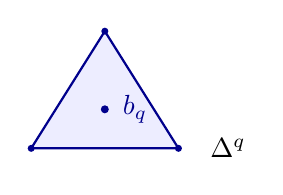
\begin{tikzpicture}[baseline=(current bounding box.center), scale=0.85]
    \coordinate (V0) at (0, 0);
    \coordinate (V1) at (2.2, 0);
    \coordinate (V2) at (1.1, 1.75);
    \coordinate (B)  at (1.1, 0.583);

    \fill[blue!7] (V0) -- (V1) -- (V2) -- cycle;
    \draw[thick, blue!55!black] (V0) -- (V1) -- (V2) -- cycle;
    \foreach \V in {V0, V1, V2} {
        \fill[blue!55!black] (\V) circle (1.5pt);
    }
    \fill[blue!55!black] (B) circle (1.7pt) node[right=3pt] {$b_q$};
    \node[right=8pt] at (V1) {$\Delta^q$};
\end{tikzpicture}
\]
Definimos por recursión las cadenas afines $\mathcal{S}_q \in S_q(\Delta^q)$ poniendo
\[
\mathcal{S}_0 = \operatorname{Id}_{\Delta^0} \in S_0(\Delta^0)
\qquad \text{y} \qquad
\mathcal{S}_q \equiv b_q \cdot \sum_{i=0}^q (-1)^i (F_q^i)_\#(\mathcal{S}_{q-1}) \quad (q > 0).
\]
Si denotamos $z_{q-1} \equiv \sum_{i=0}^q (-1)^i (F_q^i)_\#(\mathcal{S}_{q-1})$, se prueba por inducción sobre $q$ que $z_{q-1}$ es un ciclo usando las identidades de caras $F_q^i \circ F_{q-1}^j = F_q^j \circ F_{q-1}^{i-1}$ para $j < i$. Aplicando entonces el lema de la construcción cono, resulta
\[
\partial_q(\mathcal{S}_q) =
\begin{cases}
0 & \text{si } q = 0, \\
z_{q-1} & \text{si } q > 0.
\end{cases}
\]
Con las cadenas $\mathcal{S}_q$ ya construidas, definimos $\operatorname{sd}_q^X \colon S_q(X) \to S_q(X)$ sobre cada $q$-simplejo singular $\sigma \colon \Delta^q \to X$ mediante
\[
\operatorname{sd}_q^X(\sigma) = \sigma_\#(\mathcal{S}_q),
\]
y lo extendemos por linealidad a todo $S_q(X)$.

\begin{ejercicio}
    % ID: 76
Ver que $\operatorname{sd} = \{\operatorname{sd}_q^X\}$ es una transformación natural.
\end{ejercicio}

\smallskip
\noindent\textit{Paso 4.} Se comprueba por inducción sobre $q$ que $\operatorname{sd}_*^X = \{\operatorname{sd}_q^X\}_{q \geq 0}$ es un morfismo de cadenas. Además, se tiene que $\operatorname{sd}_*^X \underset{c}{\simeq} \operatorname{Id}_{S_*(X)}$; para ello se construye una homotopía de cadenas natural $h_q^X \colon S_q(X) \to S_{q+1}(X)$, de manera que
\[
(\operatorname{sd}^X)_* = \operatorname{Id} \colon H_*(X; R) \longrightarrow H_*(X; R),
\]
es decir, $[\operatorname{sd}_q^X(z)] = [z]$ para todo ciclo $z$.

\smallskip
\noindent\textit{Paso 5.} Dado un $q$-simplejo singular $\sigma \colon \Delta^q \to X$, consideremos la cubierta abierta de $\Delta^q$ dada por $\{\sigma^{-1}(\mathring{U}_\alpha)\}_{\alpha \in \Lambda}$, donde $X = \bigcup_{\alpha \in \Lambda} \mathring{U}_\alpha$. Usando el número de Lebesgue y el hecho de que al iterar el operador subdivisión los simplejos singulares resultantes se hacen arbitrariamente pequeños, existe $r \geq 0$ tal que, denotando por
\[
{}^r\operatorname{sd}_q^X \equiv \underbrace{\operatorname{sd}_q^X \circ \operatorname{sd}_q^X \circ \cdots \circ \operatorname{sd}_q^X}_{r \text{ veces}},
\]
se cumple ${}^r\operatorname{sd}_q^X(\sigma) \in S_q^{\mathcal{U}}(X)$. Para cada $\sigma \colon \Delta^q \to X$, definimos $r(\sigma) \geq 0$ como el menor entero tal que ${}^{r(\sigma)}\operatorname{sd}_q^X(\sigma) \in S_q^{\mathcal{U}}(X)$, con la convención ${}^0\operatorname{sd}_q^X(\sigma) = \sigma$.

\smallskip
\noindent\textit{Paso 6.} Para definir $\tau_q \colon S_q(X) \to S_q^{\mathcal{U}}(X)$, lo más sencillo sería poner $\tau_q(\sigma) = {}^{r(\sigma)}\operatorname{sd}_q^X(\sigma)$; sin embargo, con esta definición $\tau$ no resulta ser un morfismo de cadenas. Para dar la definición adecuada, recordemos que buscamos morfismos
\[
\begin{tikzcd}[column sep=2.6em]
S_q^{\mathcal{U}}(X) \arrow[r, hook, "i"] & S_q(X) \arrow[r, "\tau"] & S_q^{\mathcal{U}}(X)
\end{tikzcd}
\]
que satisfagan $\tau \circ i = \operatorname{Id}_{S_*^{\mathcal{U}}(X)}$ y $i \circ \tau \underset{c}{\simeq} \operatorname{Id}_{S_*(X)}$. Con este fin definimos una homotopía de cadenas natural $R_q^X \colon S_q(X) \to S_{q+1}(X)$ mediante
\[
R_q^X(\sigma) = \sum_{0 \leq j \leq r(\sigma) - 1} h_q^X\!\left({}^j\operatorname{sd}_q^X(\sigma)\right),
\]
y a partir de ella definimos
\[
\tau_q(\sigma) = R_{q-1}^X \circ \partial_q(\sigma) + \partial_{q+1} \circ R_q^X(\sigma) + \sigma.
\]
De este modo se obtiene que $i \circ \tau \underset{c}{\simeq} \operatorname{Id}_{S_*(X)}$ y $\tau \circ i = \operatorname{Id}_{S_*^{\mathcal{U}}(X)}$, por lo que la inclusión
\[
\begin{tikzcd}[column sep=2.6em]
S_*^{\mathcal{U}}(X) \arrow[r, hook, "i", "\simeq"'] & S_*(X)
\end{tikzcd}
\]
es una equivalencia homotópica de cadenas.
\end{dem}

\begin{coro}[Teorema de Escisión]
Sea $(X, A)$ una pareja de espacios topológicos y sean $U \subset A \subset X$ tales que $\overline{U} \subset \mathring{A}$. Entonces la inclusión $j \colon (X - U, A - U) \hookrightarrow (X, A)$ induce isomorfismos
\[
j_* \colon H_q(X - U, A - U; R) \xrightarrow{\;\cong\;} H_q(X, A; R)
\]
para todo $q \geq 0$.
\end{coro}
\begin{dem}
Consideremos la familia de subconjuntos $\mathcal{U} = \{X - U, A\}$ de $X$. Por hipótesis, $\overline{U} \subset \mathring{A}$, de modo que
\[
X = (X - \overline{U}) \cup \mathring{A} = (X - U)^\circ \cup \mathring{A}.
\]
En este caso, $S_*^{\mathcal{U}}(X) = S_*(X - U) + S_*(A)$, y por el teorema anterior la inclusión
\[
\begin{tikzcd}[column sep=2.8em]
S_*^{\mathcal{U}}(X) = S_*(X - U) + S_*(A) \arrow[r, hook, "i", "\underset{c}{\simeq}"'] & S_*(X)
\end{tikzcd}
\]
es una equivalencia homotópica de cadenas.

Claramente, para cualesquiera subespacios $A, B \subset X$ se cumple $S_*(A \cap B) = S_*(A) \cap S_*(B)$; en particular,
\[
S_*(X - U) \cap S_*(A) = S_*\bigl((X - U) \cap A\bigr) = S_*(A - U).
\]
Por definición,
\[
H_*(X - U, A - U; R) \equiv H_*\bigl(S_*(X - U)/S_*(A - U)\bigr)
\quad \text{y} \quad
H_*(X, A; R) \equiv H_*\bigl(S_*(X)/S_*(A)\bigr),
\]
por lo que queremos ver que el morfismo inducido
\[
\bar{j}_\# \colon S_*(X - U)/S_*(A - U) \longrightarrow S_*(X)/S_*(A)
\]
induce un isomorfismo en homología.

Por el teorema anterior, existe un morfismo de cadenas $\tau$ tal que $\tau \circ i = \operatorname{Id}_{S_*^{\mathcal{U}}(X)}$:
\[
\begin{tikzcd}[column sep=3.0em]
S_*(X) \arrow[r, shift left=0.6ex, "\tau"] & S_*(X - U) + S_*(A). \arrow[l, hook, shift left=0.6ex, "i"]
\end{tikzcd}
\]
Como tanto $i$ como $\tau$ envían $S_*(A)$ en $S_*(A)$, ambos pasan a los cocientes y obtenemos
\[
\begin{tikzcd}[column sep=3.0em]
\bigl(S_*(X - U) + S_*(A)\bigr)\big/S_*(A) \arrow[r, shift left=0.6ex, "\bar{i}"] & S_*(X)/S_*(A). \arrow[l, shift left=0.6ex, "\bar{\tau}"]
\end{tikzcd}
\]
Además, por naturalidad, la homotopía de cadenas $R^X$ también pasa a los cocientes y define
\[
\overline{R}_q^X \colon S_q(X)/S_q(A) \longrightarrow S_{q+1}(X)/S_{q+1}(A),
\]
de manera que $\bar{i}$ y $\bar{\tau}$ son inversos homotópicos de cadenas.

Consideremos ahora el diagrama conmutativo
\[
\begin{tikzcd}[column sep=3.4em, row sep=2.8em]
S_*(X - U)/S_*(A - U)
    \arrow[r, "\bar{j}_\#"]
    \arrow[dr, "\bar{\iota}"', "\cong"{sloped}]
    & S_*(X)/S_*(A) \\
& \bigl(S_*(X - U) + S_*(A)\bigr)\big/S_*(A)
    \arrow[u, "\bar{i}"', "\underset{c}{\simeq}"]
\end{tikzcd}
\]
donde $\bar{\iota}$ es el morfismo inducido por la inclusión $\iota \colon S_*(X - U) \hookrightarrow S_*(X - U) + S_*(A)$. Por el segundo teorema de isomorfismo de $R$-módulos (Teorema de Noether), $\bar{\iota}$ es un isomorfismo de complejos de cadenas y, por tanto, induce un isomorfismo en homología. Por otro lado, $\bar{i}$ es una equivalencia homotópica de cadenas, de modo que también induce un isomorfismo en homología. En consecuencia, $j_* = (\bar{j}_\#)_*$ es un isomorfismo en homología.
\end{dem}

%%%% Clase 39 del 09/11/26 inciada el 22/11/26 terminada el 22/11/2026

%%%%%% Clase 40 del 11/11/2026 iniciada el 22/11/2026

\begin{prop}
Sea $X$ un espacio topológico y consideremos subespacios $V \subset U \subset A \subset X$ tales que:
\begin{enumerate}
    \item $V$ se puede escindir, es decir, la inclusión $\iota \colon (X - V, A - V) \hookrightarrow (X, A)$ es una escisión.
    \item $(X - U, A - U)$ es un retracto por deformación de $(X - V, A - V)$, con inclusión $j \colon (X - U, A - U) \hookrightarrow (X - V, A - V)$.
\end{enumerate}
Entonces $U$ se puede escindir, es decir, la inclusión $i \colon (X - U, A - U) \hookrightarrow (X, A)$ es una escisión.
\end{prop}

\begin{dem}
Por la condición 2, existe una función continua $r \colon (X - V, A - V) \to (X - U, A - U)$ tal que
\[
r \circ j = \operatorname{Id}_{(X - U, A - U)}
\qquad \text{y} \qquad
j \circ r \simeq \operatorname{Id}_{(X - V, A - V)}.
\]
Por la invariancia homotópica de la homología, $j_*$ es un isomorfismo en homología. Además, por la condición 1, $\iota_*$ también es un isomorfismo en homología.

Consideremos el diagrama conmutativo de inclusiones
\[
\begin{tikzcd}[column sep=0.1em, row sep=2.4em]
(X - U, A - U) \arrow[rr, "j"] \arrow[dr, "i"'] & & (X - V, A - V) \arrow[dl, "\iota"] \\
& (X, A) &
\end{tikzcd}
\]
Aplicando homología obtenemos que $i_* = \iota_* \circ j_*$ es una composición de isomorfismos y, por lo tanto, es un isomorfismo en homología; es decir, $i$ es una escisión.
\end{dem}
\begin{definicion}[Homología reducida]
Sea $X$ un espacio topológico. Definimos la \textit{homología reducida} de $X$, denotada por $\widetilde{H}_q(X; R)$, de alguna de las siguientes maneras:
\begin{enumerate}
    \item[(i)] Considerando la función constante $c \colon X \to \{\mathrm{pt}\}$ y el homomorfismo inducido $c_* \colon H_q(X; R) \to H_q(\{\mathrm{pt}\}; R)$, ponemos
    \[
    \widetilde{H}_q(X; R) \equiv \ker c_*.
    \]
    \item[(ii)] Fijando un punto $x_0 \in X$, ponemos
    \[
    \widetilde{H}_q(X; R) \equiv H_q(X, \{x_0\}; R).
    \]
\end{enumerate}
\end{definicion}

Para ver que las definiciones (i) y (ii) son isomorfas (cuando $X \neq \emptyset$) necesitamos el siguiente resultado algebraico.

\begin{prop}
Consideremos una sucesión exacta corta de $R$-módulos:
\[
\begin{tikzcd}[column sep=2.6em]
0 \arrow[r] & A \arrow[r, "i"] & B \arrow[r, "j"] \arrow[l, dashed, bend left=38, "k"] & C \arrow[r] \arrow[l, dashed, bend left=38, "l"] & 0
\end{tikzcd}
\]
Entonces son equivalentes:
\begin{enumerate}
    \item Existe un homomorfismo $k \colon B \to A$ tal que $k \circ i = \operatorname{Id}_A$ (es decir, la sucesión se escinde por la izquierda).
    \item Existe un homomorfismo $l \colon C \to B$ tal que $j \circ l = \operatorname{Id}_C$ (es decir, la sucesión se escinde por la derecha).
    \item $B \cong A \oplus C$.
\end{enumerate}
Además, si la sucesión se escinde, los homomorfismos $k$ y $l$ pueden elegirse de manera que la sucesión
\[
\begin{tikzcd}[column sep=1em]
0 \arrow[r] & C \arrow[r, "l"] & B \arrow[r, "k"] & A \arrow[r] & 0
\end{tikzcd}
\]
sea exacta.
\end{prop}

\begin{prop}
Las definiciones \textup{(i)} y \textup{(ii)} de homología reducida son isomorfas.
\end{prop}

\begin{dem}
Consideremos la sucesión exacta larga de la pareja $(X, \{x_0\})$:
\[
{\small
\begin{tikzcd}[column sep=1.9em]
\cdots \arrow[r]
& H_q(\{x_0\}; R) \arrow[r, "i_*"]
& H_q(X; R) \arrow[r, "j_*"] \arrow[l, bend left=36, "c_*"]
& H_q(X, \{x_0\}; R) \arrow[r, "\hat{\partial}_q = 0"]
& H_{q-1}(\{x_0\}; R) \arrow[r, "i_*"]
& H_{q-1}(X; R) \arrow[l, bend left=36, "c_*"]
\end{tikzcd}}
\]

Sea $c \colon X \to \{x_0\}$ la función constante. Como $c \circ i = \operatorname{Id}_{\{x_0\}}$, al aplicar homología resulta 
$$c_* \circ i_* = \operatorname{Id}_{H_q(\{x_0\}; R)}$$ 
en todos los grados.

En particular, cada $i_*$ es inyectivo; como $\operatorname{Im} \hat{\partial}_q = \ker i_* = 0$, tenemos $\hat{\partial}_q = 0$ para todo $q$. Así, la sucesión exacta larga se descompone en sucesiones exactas cortas:
\[
\begin{tikzcd}[column sep=2.8em]
0 \arrow[r]
& H_q(\{x_0\}; R) \arrow[r, "i_*"]
& H_q(X; R) \arrow[r, "j_*"] \arrow[l, bend left=38, "c_*"]
& H_q(X, \{x_0\}; R) \arrow[r] \arrow[l, bend left=38, "l"]
& 0
\end{tikzcd}
\]
Como la sucesión se escinde por la izquierda mediante $c_*$, por la proposición anterior existe un homomorfismo $l \colon H_q(X, \{x_0\}; R) \to H_q(X; R)$ inverso por la derecha de $j_*$, es decir, $j_* \circ l = \operatorname{Id}$ (en particular, $j_*$ es suprayectivo y $l$ es inyectivo), tal que además la sucesión con $l$ y $c_*$ es exacta, por lo que
\[
{\operatorname{Im} l}= {\ker c_*}.
\]
En otras palabras, $\ker c_* \cong H_q(X, \{x_0\}; R)$.
\end{dem}
\begin{corolario}
Para todo $q$ se tiene
\[
H_q(X; R) \cong \widetilde{H}_q(X; R) \oplus H_q(\{x_0\}; R).
\]
\end{corolario}

\begin{dem}
Se sigue directamente del inciso 3 de la proposición sobre sucesiones exactas escindidas.
\end{dem}

\begin{corolario}
Si $X$ es un espacio contraíble, entonces $\widetilde{H}_q(X; R) \cong 0$ para todo $q \geq 0$.
\end{corolario}

\begin{lema}
Sean $S_+^n$ y $S_-^n$ los hemisferios norte y sur de $S^n$ ($n \geq 1$). Entonces la inclusión
\[
i \colon (S_+^n, S^{n-1}) \hookrightarrow (S^n, S_-^n)
\]
es una escisión.
\end{lema}

\begin{dem}
Identifiquemos la inclusión $i \colon (S_+^n, S^{n-1}) \hookrightarrow (S^n, S_-^n)$ con $(X - U, A - U) \hookrightarrow (X, A)$ mediante
\begin{align*}
(X, A) &= (S^n, S_-^n), \\
(X - U, A - U) &= (S_+^n, S^{n-1}),
\end{align*}
donde $U$ es el hemisferio sur abierto. Como $\overline{U} = S_-^n \not\subset \mathring{A}$, no podemos aplicar directamente el Teorema de Escisión a $i$.

Consideremos entonces el casquete abierto
\[
V = \{x \in S^n \mid x_{n+1} < -1/2\}.
\]
\[
\begin{tikzpicture}[baseline=(current bounding box.center), scale=0.75]
    % === Rellenos de las regiones recortados al disco de la esfera ===
    \begin{scope}
        \clip (0, 0) circle (2.0);
        % Hemisferio norte S_+^n
        \fill[blue!5] (0, 0) circle (2.0);
        % Franja S_-^n - V (entre el ecuador y el paralelo x_{n+1} = -1/2)
        \fill[blue!11]
            (-2.1, 0) -- (-2.0, 0)
            arc[start angle=180, end angle=360, x radius=2.0, y radius=0.40]
            -- (2.1, 0) -- (2.1, -2.2) -- (-2.1, -2.2) -- cycle;
        % Casquete escindido V = {x \in S^n | x_{n+1} < -1/2}
        \fill[red!14]
            (-2.1, -1.0206) -- (-1.7200, -1.0206)
            arc[start angle=186.77, end angle=353.23, x radius=1.73205, y radius=0.34641]
            -- (2.1, -1.0206) -- (2.1, -2.2) -- (-2.1, -2.2) -- cycle;
    \end{scope}

    % === Arcos posteriores (ocultos) ===
    % Ecuador posterior
    \draw[dashed, blue!55!black!55]
        (2.0, 0) arc[start angle=0, end angle=180, x radius=2.0, y radius=0.40];
    % Paralelo x_{n+1} = -1/2 posterior
    \draw[dashed, red!55!black!55]
        (1.7200, -1.0206) arc[start angle=-6.77, end angle=186.77, x radius=1.73205, y radius=0.34641];

    % === Contorno de la esfera y arcos frontales ===
    \draw[thick, blue!55!black] (0, 0) circle (2.0);
    % Ecuador frontal S^{n-1}
    \draw[thick, blue!55!black]
        (-2.0, 0) arc[start angle=180, end angle=360, x radius=2.0, y radius=0.40];
    % Paralelo frontal x_{n+1} = -1/2
    \draw[thick, red!65!black]
        (-1.7200, -1.0206) arc[start angle=186.77, end angle=353.23, x radius=1.73205, y radius=0.34641];

    % === Flechas indicando la retracción por deformación r hacia S^{n-1} ===
    \draw[->, semithick, blue!65!black] (-0.75, -1.18) -- (-0.75, -0.48);
    \draw[->, semithick, blue!65!black] ( 0.00, -1.22) -- ( 0.00, -0.50);
    \draw[->, semithick, blue!65!black] ( 0.75, -1.18) -- ( 0.75, -0.48);
    \node[blue!65!black] at (0.24, -0.88) {\scriptsize $r$};

    % === Etiquetas distribuidas sin cruces ===
    \node[blue!55!black] at (0,  1.08) {$S_+^n$};
    \node[red!65!black]  at (0, -1.66) {$V$};

    % Ecuador y paralelo a la derecha
    \node[blue!55!black, right=4pt] at (2.0, 0) {$S^{n-1}$};
    \draw[thin, red!55!black!70] (1.76, -1.0206) -- (1.96, -1.0206);
    \node[red!65!black, right=2pt] at (1.96, -1.0206) {\scriptsize $x_{n+1} = -\tfrac{1}{2}$};

    % Hemisferio sur S_-^n acotado limpiamente a la izquierda
    \draw[thin, blue!55!black!70, rounded corners=2pt]
        (-2.12, -0.04) -- (-2.26, -0.04) -- (-2.26, -1.96) -- (-2.12, -1.96);
    \node[blue!55!black, left=3pt] at (-2.26, -1.00) {$S_-^n$};
\end{tikzpicture}
\]
Como $\overline{V} \subset \mathring{A}$, por el Teorema de Escisión $V$ se puede escindir. Además, tenemos una retracción por deformación
\[
\begin{tikzcd}[column sep=2.8em]
(S^n - V, S_-^n - V) \arrow[r, shift left=0.6ex, "r"] & (S_+^n, S^{n-1}), \arrow[l, hook, shift left=0.6ex, "j"]
\end{tikzcd}
\]
de modo que $(S_+^n, S^{n-1})$ es un retracto por deformación de $(S^n - V, S_-^n - V)$ vía la inclusión $j$. Por la proposición posterior al Teorema de Escisión, concluimos que $i$ es una escisión.
\end{dem}

\begin{ejercicio}
    % ID: 77
Consideremos el \textit{complejo de cadenas aumentado} de $X$:
\[
\begin{tikzcd}[column sep=1.7em]
\cdots \arrow[r] & S_q(X) \arrow[r] & S_{q-1}(X) \arrow[r] & \cdots \arrow[r] & S_2(X) \arrow[r, "\partial_2"] & S_1(X) \arrow[r, "\partial_1"] & S_0(X) \arrow[r, "\varepsilon"] & R \arrow[r] & 0.
\end{tikzcd}
\]
Definiendo $\widetilde{H}_q(X; R)$ como la homología de este complejo de cadenas aumentado, se obtiene
\begin{align*}
\widetilde{H}_0(X; R) &\equiv \ker\varepsilon / \operatorname{Im}\partial_1, \\
\widetilde{H}_q(X; R) &= H_q(X; R) \qquad \text{si } q > 0.
\end{align*}
Ver que esta definición es isomorfa a cualquiera de las dos anteriores (recordemos que $\operatorname{Im}\partial_1 \subset \ker\varepsilon$).
\end{ejercicio}

\begin{ejercicio}
    % ID: 78
Ver que para una pareja $(X, A)$ con $A \neq \emptyset$ tenemos una sucesión exacta larga en homología reducida:
\[
\begin{tikzcd}[column sep=2.2em, row sep=1.8em]
\cdots \arrow[r] & \widetilde{H}_q(A; R) \arrow[r] & \widetilde{H}_q(X; R) \arrow[r] & H_q(X, A; R) \arrow[r] & \widetilde{H}_{q-1}(A; R) \arrow[r] & \cdots \\
& \cdots \arrow[r] & \widetilde{H}_0(A; R) \arrow[r, "i_*"] & \widetilde{H}_0(X; R) \arrow[r, "j_*"] & H_0(X, A; R) \arrow[r] & 0.
\end{tikzcd}
\]
\end{ejercicio}
\begin{prop}
Para todo $n \geq 0$ se tiene
\[
\widetilde{H}_q(S^n; R) \cong
\begin{cases}
R & \text{si } q = n, \\
0 & \text{si } q \neq n.
\end{cases}
\]
\end{prop}

\begin{dem}
Para $n \geq 1$, consideremos primero la sucesión exacta larga en homología reducida de la pareja $(D^n, S^{n-1})$:
\[
{\small
\begin{tikzcd}[column sep=1.6em, row sep=1.0em]
\cdots \arrow[r]
& \widetilde{H}_q(S^{n-1}; R) \arrow[r]
& \widetilde{H}_q(D^n; R) \arrow[r] \arrow[d, phantom, "\cong"{description, sloped, inner sep=1pt}]
& H_q(D^n, S^{n-1}; R) \arrow[r, "\hat{\partial}_q", "\cong"']
& \widetilde{H}_{q-1}(S^{n-1}; R) \arrow[r]
& \widetilde{H}_{q-1}(D^n; R) \arrow[d, phantom, "\cong"{description, sloped, inner sep=1pt}] \\
& & 0 & & & 0
\end{tikzcd}}
\]
donde las homologías reducidas de $D^n$ se anulan ya que $D^n \simeq \{*\}$ es contraíble; por exactitud, $\hat{\partial}_q$ es un isomorfismo.

Por otro lado, la proyección $\pi \colon (S_+^n, S^{n-1}) \xrightarrow{\;\cong\;} (D^n, S^{n-1})$ es un homeomorfismo de parejas. Consideremos ahora la sucesión exacta larga en homología reducida de la pareja $(S^n, S_-^n)$:
\[
\begin{tikzcd}[column sep=2.2em, row sep=1.0em]
\widetilde{H}_q(S_-^n; R) \arrow[r] \arrow[d, phantom, "\cong"{description, sloped, inner sep=1pt}]
& \widetilde{H}_q(S^n; R) \arrow[r, "j_*", "\cong"']
& H_q(S^n, S_-^n; R) \arrow[r]
& \widetilde{H}_{q-1}(S_-^n; R) \arrow[r] \arrow[d, phantom, "\cong"{description, sloped, inner sep=1pt}]
& \cdots \\
0 & & & 0
\end{tikzcd}
\]
donde $\widetilde{H}_*(S_-^n; R) = 0$ por ser $S_-^n$ contraíble, de modo que $j_*$ es un isomorfismo.

Combinando estos resultados con el lema de escisión para $i \colon (S_+^n, S^{n-1}) \hookrightarrow (S^n, S_-^n)$, tenemos el diagrama
\[
\begin{tikzcd}[column sep=3.4em, row sep=2.2em]
\widetilde{H}_q(S^n; R)
    \arrow[r, "j_*", "\cong"']
    \arrow[dd, dashed, "\Sigma"', "\cong"]
    & H_q(S^n, S_-^n; R) \\
    & H_q(S_+^n, S^{n-1}; R)
        \arrow[u, "i_*"', "\cong"]
        \arrow[d, "\pi_*", "\cong"'] \\
\widetilde{H}_{q-1}(S^{n-1}; R)
    & H_q(D^n, S^{n-1}; R)
        \arrow[l, "\hat{\partial}_q", "\cong"']
\end{tikzcd}
\]
obteniendo así el \textit{isomorfismo de suspensión}
\[
\Sigma = \hat{\partial}_q \circ \pi_* \circ i_*^{-1} \circ j_* \colon \widetilde{H}_q(S^n; R) \xrightarrow{\;\cong\;} \widetilde{H}_{q-1}(S^{n-1}; R).
\]
Procedemos ahora por inducción sobre $n$. Para el caso base $n = 0$, tenemos
\begin{align*}
\widetilde{H}_q(S^0; R) &\cong H_q(S^0, \{-1\}; R) \\
&\cong H_q(\{1\}; R) \qquad \text{(por escisión)} \\
&\cong
\begin{cases}
R & \text{si } q = 0, \\
0 & \text{si } q \neq 0.
\end{cases}
\end{align*}

Supongamos ahora que tenemos el resultado para $n - 1$. Aplicando el isomorfismo de suspensión $\Sigma$ junto con la hipótesis de inducción, resulta
\[
\widetilde{H}_q(S^n; R) \underset{\Sigma}{\cong} \widetilde{H}_{q-1}(S^{n-1}; R) \cong
\begin{cases}
R & \text{si } q - 1 = n - 1, \\
0 & \text{si } q - 1 \neq n - 1,
\end{cases}
\]
es decir, $R$ si $q = n$ y $0$ si $q \neq n$.
\end{dem}
%%%% Clase 40 del 11/11/26 inciada el 22/11/26 terminada el 24/11/2026

%%%%%% Clase 41 del 13/11/2026 iniciada el 24/11/2026
\subsection{Aplicaciones}
\begin{corolario}
Si $n \neq m$, entonces $S^n \not\simeq S^m$.
\end{corolario}

\begin{dem}
Supongamos que existe una equivalencia homotópica $f \colon S^n \to S^m$. Tomando un anillo no trivial $R \neq 0$, el homomorfismo inducido en homología reducida de grado $n$ da un isomorfismo
\[
\begin{tikzcd}[column sep=3.0em, row sep=1.0em]
\widetilde{H}_n(S^n; R)
    \arrow[r, "f_*", "\cong"']
    \arrow[d, phantom, "\cong"{description, sloped, inner sep=1pt}]
& \widetilde{H}_n(S^m; R)
    \arrow[d, phantom, "\cong"{description, sloped, inner sep=1pt}] \\
R & 0
\end{tikzcd}
\]
lo cual es una contradicción. Por lo tanto, no existe tal equivalencia homotópica $f$.
\end{dem}

\begin{teorema}[Invariancia de la dimensión (Brouwer)]
Si $n \neq m$, entonces $\mathbb{R}^n$ no es homeomorfo a $\mathbb{R}^m$.
\end{teorema}

\begin{dem}
Si alguno de los índices es $0$, el resultado es inmediato por cardinalidad; supongamos entonces $n, m \geq 1$ y que existe un homeomorfismo $h \colon \mathbb{R}^n \xrightarrow{\;\cong\;} \mathbb{R}^m$. Componiendo $h$ con una traslación en $\mathbb{R}^m$, obtenemos un homeomorfismo $f \colon \mathbb{R}^n \xrightarrow{\;\cong\;} \mathbb{R}^m$ tal que $f(0) = 0$.

Al restringir $f$ al complemento del origen, consideremos el diagrama
\[
\begin{tikzcd}[column sep=3.4em, row sep=2.5em]
\mathbb{R}^n - \{0\} \arrow[r, "f|_{\mathbb{R}^n - \{0\}}", "\cong"'] & \mathbb{R}^m - \{0\} \\
S^{n-1} \arrow[u, hook, "i", "\simeq"'] \arrow[r, dashed, "\simeq"'] & S^{m-1} \arrow[u, hook, "j"', "\simeq"]
\end{tikzcd}
\]
donde las inclusiones $i$ y $j$ son equivalencias homotópicas (en particular, retractos por deformación). Al componer con $i$, $f|_{\mathbb{R}^n - \{0\}}$ y un inverso homotópico de $j$, obtenemos una equivalencia homotópica $S^{n-1} \simeq S^{m-1}$, lo cual contradice el corolario anterior. Por consiguiente, $\mathbb{R}^n \not\cong \mathbb{R}^m$.
\end{dem}

\begin{ejercicio}
    % ID: 79
Ver que la inclusión $i \colon S^{n-1} \hookrightarrow \mathbb{R}^n - \{0\}$ es un retracto por deformación.
\end{ejercicio}

\begin{prop}
Para todo $n \geq 1$, la esfera $S^{n-1}$ no es un retracto de $D^n$.
\end{prop}

\begin{dem}
Supongamos que existe una retracción $r \colon D^n \to S^{n-1}$, de manera que para la inclusión $i \colon S^{n-1} \hookrightarrow D^n$ se cumple $r \circ i = \operatorname{Id}_{S^{n-1}}$. Aplicando homología reducida con coeficientes en un anillo no trivial $R \neq 0$, tenemos
\[
r_* \circ i_* = \operatorname{Id}_{\widetilde{H}_{n-1}(S^{n-1}; R)},
\]
que se factoriza mediante el diagrama
\[
\begin{tikzcd}[column sep=3.2em, row sep=1.0em]
\widetilde{H}_{n-1}(S^{n-1}; R)
    \arrow[r, "i_*"']
    \arrow[rr, bend left=30, "\operatorname{Id}"]
& \widetilde{H}_{n-1}(D^n; R)
    \arrow[r, "r_*"']
    \arrow[d, phantom, "\cong"{description, sloped, inner sep=1pt}]
& \widetilde{H}_{n-1}(S^{n-1}; R) \\
& 0 &
\end{tikzcd}
\]
Como $\widetilde{H}_{n-1}(D^n; R) \cong 0$, la composición $r_* \circ i_*$ satisface simultáneamente
\[
r_* \circ i_* =
\begin{cases}
\operatorname{Id}, \\
0,
\end{cases}
\]
lo cual es una contradicción pues $\widetilde{H}_{n-1}(S^{n-1}; R) \cong R \neq 0$. Por lo tanto, no existe tal retracción $r$.
\end{dem}
\begin{teorema}[Teorema del punto fijo de Brouwer]
Sea $f \colon D^n \to D^n$ una función continua ($n \geq 1$). Entonces existe $x \in D^n$ tal que $f(x) = x$.
\end{teorema}

\begin{dem}
Supongamos que $f$ no tiene puntos fijos, es decir, $f(x) \neq x$ para todo $x \in D^n$. Para cada $x \in D^n$, consideremos el semirrayo que parte de $f(x)$ y pasa por $x$, parametrizado a partir de $x$ mediante el vector unitario
\[
u(x) = \frac{x - f(x)}{\|x - f(x)\|}, \qquad p(t) = x + t u(x) \quad (t \geq 0).
\]
Buscamos $t \geq 0$ tal que $\|p(t)\| = 1$, es decir, $p(t) \in S^{n-1}$. Elevando al cuadrado y usando que $\|u(x)\| = 1$, esto ocurre si y solo si
\begin{equation}
\label{eq: projection over Sn-1}
t^2 + 2t\langle x, u(x) \rangle + \|x\|^2 - 1 = 0.
\end{equation}
Definimos la función $t \colon D^n \to \mathbb{R}$ mediante
\[
t(x) = -\langle x, u(x) \rangle + \sqrt{\langle x, u(x) \rangle^2 + (1 - \|x\|^2)}.
\]
Como $\|x\|^2 \leq 1$ para todo $x \in D^n$, se tiene $\langle x, u(x) \rangle^2 + (1 - \|x\|^2) \geq \langle x, u(x) \rangle^2 \geq 0$, por lo que $t(x) \in \mathbb{R}$ está bien definida, cumple $t(x) \geq 0$ y satisface la ecuación~\eqref{eq: projection over Sn-1}.

Definimos ahora $r \colon D^n \to S^{n-1}$ por
\[
r(x) = x + t(x) u(x),
\]
que es la intersección del semirrayo que va de $f(x)$ a $x$ con $S^{n-1}$. Como $f$ es continua y $x - f(x) \neq 0$ en todo $D^n$, las funciones $u$ y $t$ son continuas y, en consecuencia, $r$ es continua.
\[
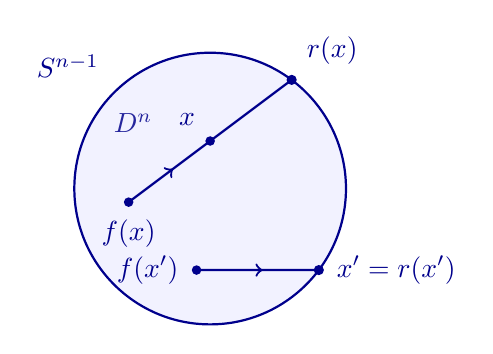
\begin{tikzpicture}[baseline=(current bounding box.center), scale=1.15]
    % Disco D^n y esfera frontera S^{n-1}
    \fill[blue!5] (0, 0) circle (1.5cm);
    \draw[thick, blue!55!black] (0, 0) circle (1.5cm);

    % Etiquetas de D^n y S^{n-1}
    \node[blue!55!black!85] at (-0.85, 0.72) {$D^n$};
    \node[blue!55!black, above left=2pt] at (-1.06, 1.06) {$S^{n-1}$};

    % === Caso 1: x en el interior de D^n ===
    \coordinate (F1) at (-0.90, -0.15);
    \coordinate (X1) at ( 0.00,  0.525);
    \coordinate (R1) at ( 0.90,  1.20);

    \draw[->, thick, blue!55!black] (F1) -- (-0.41, 0.2175);
    \draw[thick, blue!55!black] (-0.45, 0.1875) -- (R1);

    \fill[blue!55!black] (F1) circle (1.5pt) node[below=3pt] {$f(x)$};
    \fill[blue!55!black] (X1) circle (1.5pt) node[above left=2pt] {$x$};
    \fill[blue!55!black] (R1) circle (1.6pt) node[above right=2pt] {$r(x)$};

    % === Caso 2: x' en la frontera S^{n-1} ===
    \coordinate (F2) at (-0.15, -0.90);
    \coordinate (R2) at ( 1.20, -0.90);

    \draw[->, thick, blue!55!black] (F2) -- (0.58, -0.90);
    \draw[thick, blue!55!black] (0.52, -0.90) -- (R2);

    \fill[blue!55!black] (F2) circle (1.5pt) node[left=3pt] {$f(x')$};
    \fill[blue!55!black] (R2) circle (1.6pt) node[right=3pt] {$x' = r(x')$};
\end{tikzpicture}
\]
Notemos que si $x \in S^{n-1}$, entonces $\|x\| = 1$. Además, por la desigualdad de Cauchy--Schwarz y el hecho de que $\|f(x)\| \leq 1$ con $f(x) \neq x$, tenemos
\[
\langle x, x - f(x) \rangle = \|x\|^2 - \langle x, f(x) \rangle = 1 - \langle x, f(x) \rangle > 0,
\]
de donde $\langle x, u(x) \rangle > 0$. Por lo tanto,
\[
t(x) = -\langle x, u(x) \rangle + \sqrt{\langle x, u(x) \rangle^2} = -\langle x, u(x) \rangle + \langle x, u(x) \rangle = 0,
\]
y así $r(x) = x$. Es decir, $r \circ i = \operatorname{Id}_{S^{n-1}}$ para la inclusión $i \colon S^{n-1} \hookrightarrow D^n$.

En consecuencia, $r \colon D^n \to S^{n-1}$ es una retracción, lo cual contradice la proposición anterior. Por lo tanto, existe $x \in D^n$ tal que $f(x) = x$.
\end{dem}
\begin{definicion}[Grado]
Sea $f \colon S^n \to S^n$ una función continua. Consideremos el homomorfismo inducido en homología reducida
\[
\begin{tikzcd}[column sep=3.0em, row sep=1.0em]
\widetilde{H}_n(S^n; \mathbb{Z})
    \arrow[r, "f_*"]
    \arrow[d, phantom, "\cong"{description, sloped, inner sep=1pt}]
& \widetilde{H}_n(S^n; \mathbb{Z})
    \arrow[d, phantom, "\cong"{description, sloped, inner sep=1pt}] \\
\mathbb{Z} & \mathbb{Z}
\end{tikzcd}
\]
Sea $\gamma \in \widetilde{H}_n(S^n; \mathbb{Z})$ un generador; entonces existe un único $r \in \mathbb{Z}$ tal que $f_*(\gamma) = r\gamma$. Definimos el \textit{grado} de $f$ como
\[
\operatorname{gr}(f) = r.
\]
Esta definición no depende del generador elegido, ya que si tomamos el otro generador $-\gamma$, se tiene
\[
f_*(-\gamma) = -f_*(\gamma) = -r\gamma = r(-\gamma).
\]
\end{definicion}

\begin{prop}
Si $f, g \colon S^n \to S^n$ son funciones continuas tales que $f \simeq g$, entonces $\operatorname{gr}(f) = \operatorname{gr}(g)$.
\end{prop}

\begin{dem}
Se sigue de inmediato de la invariancia homotópica de la homología, pues $f \simeq g$ implica $f_* = g_*$.
\end{dem}

\begin{nota}
Brouwer dio la definición de grado para variedades trianguladas y luego Hopf dio la definición usando homología.
\[
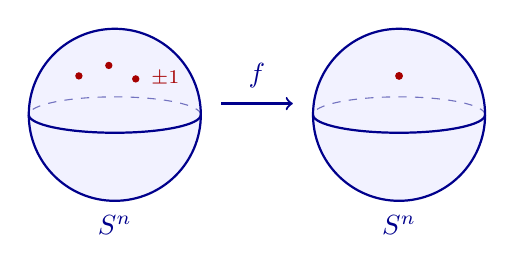
\begin{tikzpicture}[baseline=(current bounding box.center), scale=0.95]
    % === Esfera dominio S^n ===
    \fill[blue!5] (0, 0) circle (1.15);
    \draw[dashed, blue!55!black!55]
        (1.15, 0) arc[start angle=0, end angle=180, x radius=1.15, y radius=0.24];
    \draw[thick, blue!55!black] (0, 0) circle (1.15);
    \draw[thick, blue!55!black]
        (-1.15, 0) arc[start angle=180, end angle=360, x radius=1.15, y radius=0.24];
    \node[blue!55!black] at (0, -1.48) {$S^n$};

    % Preimágenes con signo \pm 1
    \fill[red!65!black] (-0.48, 0.52) circle (1.4pt);
    \fill[red!65!black] (-0.08, 0.66) circle (1.4pt);
    \fill[red!65!black] ( 0.28, 0.48) circle (1.4pt)
        node[right=2pt] {\scriptsize $\pm 1$};

    % === Flecha f ===
    \draw[->, thick, blue!55!black] (1.42, 0.15) -- (2.38, 0.15)
        node[midway, above=2pt] {$f$};

    % === Esfera codominio S^n ===
    \fill[blue!5] (3.80, 0) circle (1.15);
    \draw[dashed, blue!55!black!55]
        (4.95, 0) arc[start angle=0, end angle=180, x radius=1.15, y radius=0.24];
    \draw[thick, blue!55!black] (3.80, 0) circle (1.15);
    \draw[thick, blue!55!black]
        (2.65, 0) arc[start angle=180, end angle=360, x radius=1.15, y radius=0.24];
    \node[blue!55!black] at (3.80, -1.48) {$S^n$};

    % Punto imagen
    \fill[red!65!black] (3.80, 0.52) circle (1.5pt);
\end{tikzpicture}
\]
\end{nota}
\begin{ejercicio}
    % ID: 80
Ver que el homomorfismo de conexión
\[
\hat{\partial}_q^{(X, A)} \colon H_q(X, A; R) \longrightarrow H_{q-1}(A; R)
\]
es una transformación natural.
\end{ejercicio}

\begin{prop}
Sea $\rho \colon S^n \to S^n$ la reflexión dada por
\[
\rho(x_0, x_1, \dots, x_n) = (-x_0, x_1, \dots, x_n).
\]
Entonces el homomorfismo inducido $\rho_* \colon \widetilde{H}_n(S^n; R) \to \widetilde{H}_n(S^n; R)$ es multiplicar por $-1$; en particular (para $R = \mathbb{Z}$), $\operatorname{gr}(\rho) = -1$.
\end{prop}

\begin{dem}
Procedemos por inducción sobre $n$.

\smallskip
\noindent\textit{Caso base ($n = 0$).} Tomemos $S^0 = \{a, b\}$ (con $\rho(a) = b$ y $\rho(b) = a$) y consideremos el extremo del complejo de cadenas aumentado de $S^0$:
\[
\begin{tikzcd}[column sep=2.6em]
S_1(S^0) \arrow[r, "\partial_1"] & S_0(S^0) \arrow[r, "\varepsilon"] & R.
\end{tikzcd}
\]
Como $\Delta^1$ es conexo y $S^0 = \{a, b\}$ es discreto, los únicos $1$-simplejos singulares $\Delta^1 \to \{a, b\}$ son los constantes $c_a$ y $c_b$, que satisfacen
\[
\partial_1(c_a) = a - a = 0
\qquad \text{y} \qquad
\partial_1(c_b) = b - b = 0.
\]
En consecuencia, $\partial_1 = 0$ y $\operatorname{Im}\partial_1 = 0$. Dado que $S_0(\{a, b\}) = \{\alpha a + \beta b \mid \alpha, \beta \in R\}$, obtenemos
\[
\widetilde{H}_0(S^0; R) = \ker\varepsilon / \operatorname{Im}\partial_1 = \ker\varepsilon = \{\alpha a + \beta b \mid \alpha + \beta = 0\}.
\]

Por otro lado, para cualquier función continua $f \colon X \to Y$, la aumentación $\varepsilon$ satisface el diagrama conmutativo
\[
\begin{tikzcd}[column sep=2.6em, row sep=2.2em]
S_0(X) \arrow[r, "\varepsilon"] \arrow[d, "f_\#"'] & R \\
S_0(Y) \arrow[ur, "\varepsilon"'] &
\end{tikzcd}
\]
de modo que $f_\#$ restringe a $\ker\varepsilon$. En nuestro caso, como $\operatorname{Im}\partial_1 = 0$, el homomorfismo inducido $\rho_*$ coincide con la restricción $\rho_\#|_{\ker\varepsilon}$:
\[
\begin{tikzcd}[column sep=1em, row sep=2.0em]
\widetilde{H}_0(S^0; R) \arrow[r, phantom, "="] \arrow[d, "\rho_*"'] & \ker\varepsilon \arrow[d, "\rho_\#|_{\ker\varepsilon}"] \\
\widetilde{H}_0(S^0; R) \arrow[r, phantom, "="] & \ker\varepsilon
\end{tikzcd}
\]
Así, para todo $\alpha a + \beta b \in \ker\varepsilon$ (donde $\alpha + \beta = 0$, es decir, $\alpha = -\beta$ y $\beta = -\alpha$), tenemos
\begin{align*}
\rho_*(\alpha a + \beta b) &= \rho_\#(\alpha a + \beta b) \\
&= \alpha\rho_\#(a) + \beta\rho_\#(b) \\
&= \alpha b + \beta a \\
&= -\beta b - \alpha a \\
&= -(\alpha a + \beta b).
\end{align*}
Por lo tanto, $\rho_*$ es multiplicar por $-1$ en dimensión $0$.
\smallskip
\noindent\textit{Paso inductivo.} Sea $n \geq 1$ y supongamos que $\rho_*$ es multiplicar por $(-1)$ en dimensión $n - 1$. Veremos que el isomorfismo de suspensión $\Sigma$ conmuta con $\rho_*$, de modo que conmuta el cuadrado de la izquierda:
\[
\begin{tikzcd}[column sep=3.2em, row sep=2.8em, baseline=(current bounding box.center)]
\widetilde{H}_n(S^n; R)
    \arrow[r, "\rho_*"]
    \arrow[d, "\Sigma"', "\cong"]
& \widetilde{H}_n(S^n; R)
    \arrow[d, "\Sigma", "\cong"'] \\
\widetilde{H}_{n-1}(S^{n-1}; R)
    \arrow[r, "\rho_*"']
& \widetilde{H}_{n-1}(S^{n-1}; R)
\end{tikzcd}
\hspace{2.2em}
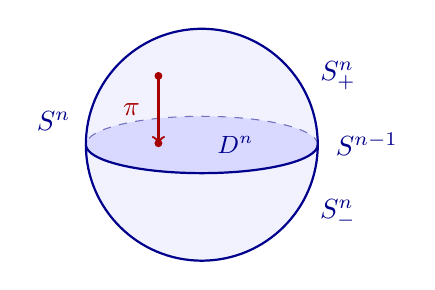
\begin{tikzpicture}[baseline=(current bounding box.center), scale=0.95]
    % Esfera S^n y disco ecuatorial D^n
    \fill[blue!5] (0, 0) circle (1.55);
    \fill[blue!15] (0, 0) ellipse [x radius=1.55, y radius=0.38];

    % Arco posterior del ecuador S^{n-1}
    \draw[dashed, blue!55!black!55]
        (1.55, 0) arc[start angle=0, end angle=180, x radius=1.55, y radius=0.38];

    % Contorno de S^n y arco frontal del ecuador
    \draw[thick, blue!55!black] (0, 0) circle (1.55);
    \draw[thick, blue!55!black]
        (-1.55, 0) arc[start angle=180, end angle=360, x radius=1.55, y radius=0.38];

    % Proyección vertical \pi de S_+^n sobre D^n
    \draw[->, thick, red!65!black] (-0.58, 0.92) -- (-0.58, 0.02)
        node[midway, left=3pt] {$\pi$};
    \fill[red!65!black] (-0.58, 0.92) circle (1.5pt);
    \fill[red!65!black] (-0.58, 0.02) circle (1.5pt);

    % Etiquetas
    \node[blue!55!black] at ( 0.45,  0.00) {\small $D^n$};
    \node[blue!55!black] at (-1.98,  0.32) {$S^n$};
    \node[blue!55!black] at ( 1.82,  0.92) {$S_+^n$};
    \node[blue!55!black, right=3pt] at (1.55, 0) {$S^{n-1}$};
    \node[blue!55!black] at ( 1.82, -0.92) {$S_-^n$};
\end{tikzpicture}
\]

Observemos que, al cambiar de signo únicamente la primera coordenada $x_0$, la reflexión $\rho \colon S^n \to S^n$ preserva $S_+^n$, $S_-^n$ y $S^{n-1}$, y se extiende con la misma fórmula al disco ecuatorial
\[
D^n = \{x \in \mathbb{R}^{n+1} \mid \|x\| \leq 1,\; x_n = 0\} \xrightarrow{\;\rho\;} D^n.
\]
Además, $\rho$ conmuta con las inclusiones $j, i$ y con la proyección
\[
\pi \colon S_+^n \longrightarrow D^n, \qquad \pi(x_0, x_1, \dots, x_n) = (x_0, x_1, \dots, x_{n-1}, 0).
\]
Por funtorialidad de la homología y por la naturalidad del homomorfismo de conexión $\hat{\partial}_n$, todos los cuadrados del siguiente diagrama conmutan:
\[
\begin{tikzcd}[column sep=4.2em, row sep=2.4em]
\widetilde{H}_n(S^n; R)
    \arrow[r, "\rho_*"]
    \arrow[d, "j_*"', "\cong"]
& \widetilde{H}_n(S^n; R)
    \arrow[d, "j_*", "\cong"'] \\
H_n(S^n, S_-^n; R)
    \arrow[r, "\rho_*"]
& H_n(S^n, S_-^n; R) \\
H_n(S_+^n, S^{n-1}; R)
    \arrow[r, "\rho_*"]
    \arrow[u, "i_*", "\cong"']
    \arrow[d, "\pi_*"', "\cong"]
& H_n(S_+^n, S^{n-1}; R)
    \arrow[u, "i_*"', "\cong"]
    \arrow[d, "\pi_*", "\cong"'] \\
H_n(D^n, S^{n-1}; R)
    \arrow[r, "\rho_*"]
    \arrow[d, "\hat{\partial}_n"', "\cong"]
& H_n(D^n, S^{n-1}; R)
    \arrow[d, "\hat{\partial}_n", "\cong"'] \\
\widetilde{H}_{n-1}(S^{n-1}; R)
    \arrow[r, "\rho_*"']
& \widetilde{H}_{n-1}(S^{n-1}; R)
\end{tikzcd}
\]
En consecuencia, $\Sigma = \hat{\partial}_n \circ \pi_* \circ i_*^{-1} \circ j_*$ conmuta con $\rho_*$, es decir, $\Sigma \circ \rho_* = \rho_* \circ \Sigma$. Como $\Sigma$ es un isomorfismo y, por hipótesis de inducción, $\rho_*$ es multiplicar por $(-1)$ en $\widetilde{H}_{n-1}(S^{n-1}; R)$, concluimos que $\rho_*$ es multiplicar por $(-1)$ en dimensión $n$.
\end{dem}

\begin{prop}
Toda rotación en $\mathbb{R}^n$, restringida como función $S^{n-1} \to S^{n-1}$, es homotópica a la identidad.
\end{prop}

\begin{dem}
Una rotación es un elemento $L \in \mathrm{SO}(n)$, es decir, una matriz tal que $L L^t = \operatorname{Id}$ y $\det(L) = 1$. Por la forma canónica de matrices ortogonales especiales, se tiene que
\[
L = Q P Q^t,
\]
donde $Q \in \mathrm{O}(n)$ y $P$ es una matriz diagonal por bloques en la que cada bloque es igual a
\[
\begin{pmatrix}
\cos\theta_i & -\operatorname{sen}\theta_i \\
\operatorname{sen}\theta_i & \cos\theta_i
\end{pmatrix}
\qquad \text{o} \qquad 1,
\]
para ciertos ángulos $\theta_i$ ($i = 1, \dots, r$).

Definimos una trayectoria $\sigma \colon I \to \mathrm{SO}(n) \subset M(n, \mathbb{R}) \cong \mathbb{R}^{n^2}$ mediante
\[
\sigma(t) = Q P(t) Q^t,
\]
donde $Q$ es fija y $P(t)$ es la matriz diagonal por bloques correspondiente con bloques iguales a
\[
\begin{pmatrix}
\cos(t\theta_i) & -\operatorname{sen}(t\theta_i) \\
\operatorname{sen}(t\theta_i) & \cos(t\theta_i)
\end{pmatrix}
\qquad \text{o} \qquad 1.
\]
Como cada entrada de $P(t)$ es una función continua de $t$ y el producto de matrices es continuo, $\sigma$ es continua.

Cuando $t = 0$, tenemos $P(0) = \operatorname{Id}$ ya que $\cos 0 = 1$ y $\operatorname{sen} 0 = 0$; en consecuencia,
\begin{align*}
\sigma(0) &= Q \operatorname{Id} Q^t = \operatorname{Id}, \\
\sigma(1) &= Q P Q^t = L.
\end{align*}
Como $L \in \mathrm{SO}(n)$ es arbitraria, esto muestra que $\mathrm{SO}(n)$ es $0$-conexo.

Consideremos la función de evaluación $\operatorname{ev} \colon \operatorname{Lin}(\mathbb{R}^n, \mathbb{R}^n) \times \mathbb{R}^n \to \mathbb{R}^n$ dada por $\operatorname{ev}(\varphi, v) = \varphi(v)$. Como $\operatorname{ev}$ es bilineal (entre espacios de dimensión finita), entonces es continua.

Definimos $H \colon S^{n-1} \times I \to S^{n-1}$ mediante
\[
H(x, t) = \sigma(t)(x).
\]
Notemos que $H$ está bien definida, pues si $L \in \mathrm{SO}(n)$ y $x \in S^{n-1}$, entonces $\operatorname{ev}(L, x) = L(x) \in S^{n-1}$ ya que $L$ preserva la norma. Además, $H$ es continua al ser la composición de la fila superior del siguiente diagrama conmutativo:
\[
\begin{tikzcd}[column sep=2.0em, row sep=2.4em]
S^{n-1} \times I \arrow[r, "\operatorname{Id} \times \sigma"] &[1.0em]
S^{n-1} \times \mathrm{SO}(n) \arrow[r, "\cong"] &
\mathrm{SO}(n) \times S^{n-1} \arrow[r, dashed, "\operatorname{ev}|"] \arrow[d, hook] &
S^{n-1} \arrow[d, hook] \\
& & \operatorname{Lin}(\mathbb{R}^n, \mathbb{R}^n) \times \mathbb{R}^n \arrow[r, "\operatorname{ev}"'] & \mathbb{R}^n
\end{tikzcd}
\]
Finalmente, para todo $x \in S^{n-1}$ se cumple
\begin{align*}
H(x, 0) &= \sigma(0)(x) = \operatorname{Id}(x) = x, \\
H(x, 1) &= \sigma(1)(x) = L(x),
\end{align*}
con lo cual $L|_{S^{n-1}} \simeq \operatorname{Id}_{S^{n-1}}$.
\end{dem}

\begin{prop}
Sea $f \colon S^n \to S^n$ la restricción de una transformación ortogonal en $\mathbb{R}^{n+1}$. Entonces el homomorfismo inducido
\[
f_* \colon \widetilde{H}_n(S^n; R) \longrightarrow \widetilde{H}_n(S^n; R)
\]
es multiplicar por $\det(f)$.
\end{prop}

\begin{dem}
Como $f$ es la restricción de una transformación ortogonal, se tiene $\det(f) = \pm 1$. Si $\det(f) = 1$, entonces dicha transformación pertenece a $\mathrm{SO}(n+1)$ y, por la proposición anterior, $f \simeq \operatorname{Id}_{S^n}$. En consecuencia, $f_*$ es multiplicar por $1$, es decir, multiplicar por $\det(f)$.

Si $\det(f) = -1$, tomamos la reflexión $\rho \colon S^n \to S^n$ y obtenemos que $\rho \circ f$ es la restricción de una rotación en $\mathrm{SO}(n+1)$. Por la proposición anterior, $\rho \circ f \simeq \operatorname{Id}_{S^n}$, de donde
\[
\rho_* \circ f_* = \operatorname{Id}_{\widetilde{H}_n(S^n; R)}.
\]
Además, $\rho$ y $f$ son homeomorfismos, por lo que $\rho_*$ y $f_*$ son isomorfismos. Como ya vimos que $\rho_*(a) = -a$, se cumple $\rho_* \circ \rho_* = \operatorname{Id}_{\widetilde{H}_n(S^n; R)}$; al combinar esto con $\rho_* \circ f_* = \operatorname{Id}_{\widetilde{H}_n(S^n; R)}$ y la unicidad del inverso, resulta que $f_* = \rho_*$, que es multiplicar por $-1 = \det(f)$.
\end{dem}

\begin{corolario}
Sea $\alpha \colon S^n \to S^n$ la función antípoda, es decir, $\alpha(a) = -a$. Entonces el homomorfismo inducido $\alpha_* \colon \widetilde{H}_n(S^n; R) \to \widetilde{H}_n(S^n; R)$ es multiplicar por $(-1)^{n+1}$.
\end{corolario}

\begin{dem}
La función antípoda $\alpha$ es la restricción de $-\operatorname{Id}_{\mathbb{R}^{n+1}}$ a $S^n$, cuyo determinante es $\det(\alpha) = (-1)^{n+1}$. Por la proposición anterior, $\alpha_*$ es multiplicar por $(-1)^{n+1}$.
\end{dem}

\begin{nota}
Si $M^n$ es una variedad suave, un \textit{campo vectorial} en $M$ asocia de forma continua a cada punto $x \in M$ un vector tangente $v(x) \in T_x M$. En el caso particular de la esfera $S^n \subset \mathbb{R}^{n+1}$, el espacio tangente $T_x S^n$ en cada punto $x \in S^n$ está formado por los vectores ortogonales a $x$, como se ilustra para $n = 1$ junto con un campo vectorial tangente en $S^1$:
\[
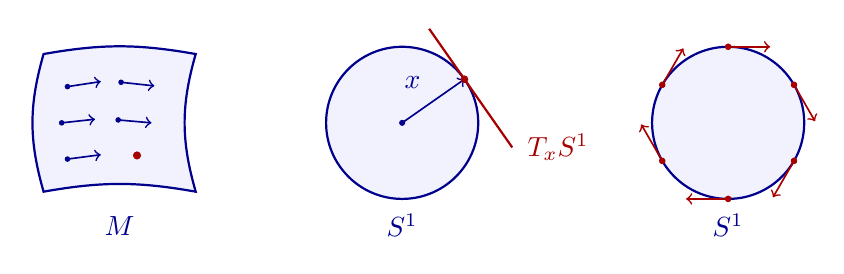
\begin{tikzpicture}[baseline=(current bounding box.center), scale=0.92]
    % === Panel 1: Variedad suave M con campo vectorial ===
    \begin{scope}
        \filldraw[thick, blue!55!black, fill=blue!5]
            (-0.95,  0.95) to[bend right=16] (-0.95, -0.95)
                           to[bend left=10]  ( 1.15, -0.95)
                           to[bend left=16]  ( 1.15,  0.95)
                           to[bend right=10] (-0.95,  0.95) -- cycle;

        \foreach \x/\y/\dx/\dy in {
            -0.62/ 0.50/0.46/ 0.07,
             0.12/ 0.56/0.46/-0.05,
            -0.70/ 0.00/0.46/ 0.05,
             0.08/ 0.04/0.46/-0.04,
            -0.62/-0.50/0.46/ 0.06
        }{
            \fill[blue!55!black] (\x, \y) circle (1.1pt);
            \draw[->, semithick, blue!55!black] (\x, \y) -- ++(\dx, \dy);
        }

        % Punto donde el campo se anula
        \fill[red!65!black] (0.34, -0.45) circle (1.6pt);
        \node[blue!55!black] at (0.10, -1.42) {$M$};
    \end{scope}

    % === Panel 2: Espacio tangente T_x S^1 ortogonal a x ===
    \begin{scope}[xshift=4.0cm]
        \filldraw[thick, blue!55!black, fill=blue!5] (0, 0) circle (1.05);
        \fill[blue!55!black] (0, 0) circle (1.2pt);

        % Vector posición x
        \draw[->, semithick, blue!55!black] (0, 0) -- (35:1.05)
            node[midway, above left=1pt] {$x$};

        % Recta tangente T_x S^1 y marca de perpendicularidad
        \begin{scope}[shift={(35:1.05)}, rotate=35]
            \draw[thick, red!65!black] (0, 0.85) -- (0, -1.15);
            %\draw[thin, red!65!black!80] (-0.16, 0) -- (-0.16, -0.16) -- (0, -0.16);
            \coordinate (Tend) at (0, -1.15);
        \end{scope}

        \fill[red!65!black] (35:1.05) circle (1.5pt);
        \node[red!65!black, right=2pt] at (Tend) {$T_x S^1$};
        \node[blue!55!black] at (0, -1.42) {$S^1$};
    \end{scope}

    % === Panel 3: Campo vectorial tangente no nulo en S^1 ===
    \begin{scope}[xshift=8.5cm]
        \filldraw[thick, blue!55!black, fill=blue!5] (0, 0) circle (1.05);

        \foreach \ang in {90, 30, -30, -90, -150, 150}{
            \begin{scope}[shift={(\ang:1.05)}, rotate=\ang]
                \draw[->, semithick, red!65!black] (0, 0) -- (0, -0.58);
                \fill[red!65!black] (0, 0) circle (1.3pt);
            \end{scope}
        }

        \node[blue!55!black] at (0, -1.42) {$S^1$};
    \end{scope}
\end{tikzpicture}
\]
\end{nota}

\begin{definicion}[Campo vectorial tangente en $S^n$]
Un \textit{campo vectorial tangente} en $S^n$ es equivalente a una función continua $v \colon S^n \to \mathbb{R}^{n+1}$ tal que $x \perp v(x)$ para todo $x \in S^n$.
\end{definicion}
%%%% Clase 41 del 13/11/26 inciada el 24/11/26 terminada el 24/11/2026

%%%%%% Clase 42 del 16/11/2026 iniciada el 24/11/2026
\begin{prop}
La esfera $S^n$ tiene un campo vectorial tangente que no se anula en ningún punto si y solo si $n$ es impar.
\end{prop}

\begin{dem}
$(\Leftarrow)$ Si $n = 2m + 1$ ($m \geq 0$), definimos $V \colon S^n \to \mathbb{R}^{n+1}$ mediante
\[
V(x_0, x_1, \dots, x_{2m+1}) = (-x_1, x_0, -x_3, x_2, \dots, -x_{2m+1}, x_{2m}).
\]
Esta función es continua, no se anula en ningún punto (ya que $\|V(x)\| = \|x\| = 1$) y cumple $x \perp V(x)$ para todo $x \in S^n$.

$(\Rightarrow)$ Supongamos que existe un campo vectorial tangente $V \colon S^n \to \mathbb{R}^{n+1}$ tal que $V(x) \neq 0$ para todo $x \in S^n$. Definimos $W \colon S^n \to S^n$ por
\[
W(x) = \frac{V(x)}{\|V(x)\|},
\]
que es continua y claramente satisface $x \perp W(x)$ para todo $x \in S^n$.

Consideremos la función continua $F \colon S^n \times I \to S^n$ dada por
\[
F(x, t) = x\cos(t\pi) + W(x)\operatorname{sen}(t\pi).
\]
Usando el producto punto (con $\|x\| = \|W(x)\| = 1$ y $\langle x, W(x) \rangle = 0$), es inmediato verificar que $\|F(x, t)\| = 1$, por lo que $F$ toma valores en $S^n$. Además, para todo $x \in S^n$ satisface
\begin{align*}
F(x, 0) &= x, \\
F(x, 1) &= -x \equiv \alpha(x),
\end{align*}
donde $\alpha \colon S^n \to S^n$ es la función antípoda. En consecuencia, $\alpha \simeq \operatorname{Id}_{S^n}$.

Aplicando homología reducida con coeficientes en $\mathbb{Z}$, el homomorfismo inducido $\alpha_* \colon \widetilde{H}_n(S^n; \mathbb{Z}) \to \widetilde{H}_n(S^n; \mathbb{Z})$ es multiplicar por $1$. Sin embargo, por el corolario anterior, $\alpha_*$ es multiplicar por $(-1)^{n+1}$. Por lo tanto, $(-1)^{n+1} = 1$, de donde concluimos que $n$ es impar.
\end{dem}
\begin{prop}
Sea $Z$ un espacio de Hausdorff y sea $Y \subset Z$ un subespacio cerrado. Supongamos que existe una función continua $F \colon (D^n, S^{n-1}) \to (Z, Y)$ tal que la restricción
\[
F|_{D^n - S^{n-1}} \colon D^n - S^{n-1} \xrightarrow{\;\cong\;} Z - Y
\]
es un homeomorfismo. Entonces
\[
Z \cong Y \cup_{F|_{S^{n-1}}} D^n.
\]
\end{prop}

\begin{dem}
Queda como ejercicio.
\end{dem}

\begin{lema}
El espacio proyectivo real $\mathbb{R}P^m \equiv S^m / \mathbb{Z}_2$ es un complejo CW con una celda de dimensión $r$ para cada $0 \leq r \leq m$.
\end{lema}

\begin{dem}
El espacio $\mathbb{R}P^m$ admite la filtración canónica
\[
\mathbb{R}P^0 = \{\mathrm{pt}\} \subset \mathbb{R}P^1 \subset \cdots \subset \mathbb{R}P^n \subset \cdots \subset \mathbb{R}P^m,
\]
donde identificamos la inclusión $\mathbb{R}P^{n-1} \hookrightarrow \mathbb{R}P^n$ con el conjunto de puntos de la forma $[x_1, x_2, \dots, x_n, 0]$.

Para cada $1 \leq n \leq m$, sea $F \colon (D^n, S^{n-1}) \to (\mathbb{R}P^n, \mathbb{R}P^{n-1})$ la composición
\[
\begin{tikzcd}[column sep=2.6em]
(D^n, S^{n-1}) \arrow[r, "\cong"] & (S_+^n, S^{n-1}) \arrow[r, hook] & (S^n, S^{n-1}) \arrow[r, "p"] & (\mathbb{R}P^n, \mathbb{R}P^{n-1}),
\end{tikzcd}
\]
donde $p$ es la proyección cociente. Explícitamente, para $x = (x_1, x_2, \dots, x_n) \in D^n$,
\[
F(x_1, x_2, \dots, x_n) = \bigl[x_1, x_2, \dots, x_n, \sqrt{1 - \|x\|^2}\bigr].
\]
La inversa de la restricción $F|_{D^n - S^{n-1}} \colon D^n - S^{n-1} \to \mathbb{R}P^n - \mathbb{R}P^{n-1}$ está dada por $\hat{F} \colon \mathbb{R}P^n - \mathbb{R}P^{n-1} \to D^n - S^{n-1}$,
\[
\hat{F}\bigl([x_1, x_2, \dots, x_{n+1}]\bigr) =
\left(
\frac{x_1 x_{n+1}}{\sqrt{\sum_{k=1}^{n+1} (x_k x_{n+1})^2}}, \dots,
\frac{x_n x_{n+1}}{\sqrt{\sum_{k=1}^{n+1} (x_k x_{n+1})^2}}
\right),
\]
que es continua y bien definida (pues $x_{n+1} \neq 0$ fuera de $\mathbb{R}P^{n-1}$). Por la proposición anterior,
\[
\mathbb{R}P^n \cong \mathbb{R}P^{n-1} \cup_{F|_{S^{n-1}}} D^n,
\]
donde la función de pegado $F|_{S^{n-1}} = p \colon S^{n-1} \to \mathbb{R}P^{n-1}$ es la proyección al cociente. Inductivamente, $\mathbb{R}P^m$ es un complejo CW con una celda de dimensión $r$ para cada $0 \leq r \leq m$.
\end{dem}

\begin{definicion}[Espacio proyectivo complejo]
Definimos el \textit{espacio proyectivo complejo} de dimensión $n$ como el espacio cociente
\[
\mathbb{C}P^n = S^{2n+1} / U(1) \cong (\mathbb{C}^{n+1} - \{0\}) / {\sim},
\]
donde $U(1) = S^1$ actúa sobre $S^{2n+1}$ mediante $U(1) \times S^{2n+1} \to S^{2n+1}$,
\[
z \cdot (z_1, \dots, z_{n+1}) = (z z_1, \dots, z z_{n+1}).
\]
\end{definicion}

\begin{lema}
El espacio proyectivo complejo $\mathbb{C}P^m$ es un complejo CW con una celda de dimensión $2r$ para cada $0 \leq r \leq m$.
\end{lema}

\begin{dem}
Tenemos la filtración canónica, donde denotamos cada $k$-esqueleto por $X^k$:
\[
X^0 = \mathbb{C}P^0 = \{\mathrm{pt}\} = X^1 \subset X^2 = \mathbb{C}P^1 = X^3 \subset X^4 = \mathbb{C}P^2 \subset \cdots \subset X^{2m} = \mathbb{C}P^m,
\]
en la que cada inclusión $\mathbb{C}P^{n-1} \hookrightarrow \mathbb{C}P^n$ está formada por los puntos de la forma $[z_1, z_2, \dots, z_n, 0]$.

Para cada $1 \leq n \leq m$, consideremos la función continua $F \colon (D^{2n}, S^{2n-1}) \to (\mathbb{C}P^n, \mathbb{C}P^{n-1})$ definida por
\[
F(x_1, x_2, \dots, x_{2n-1}, x_{2n}) =
\left[
x_1 + i x_2, \dots, x_{2n-1} + i x_{2n}, \sqrt{1 - \sum_{k=1}^{2n} x_k^2}
\right].
\]
La inversa de $F|_{D^{2n} - S^{2n-1}}$ es la función continua $\hat{F} \colon \mathbb{C}P^n - \mathbb{C}P^{n-1} \to D^{2n} - S^{2n-1}$ dada por
\[
\hat{F}\bigl([z_1, \dots, z_{n+1}]\bigr) =
\left(
\frac{\operatorname{Re}(z_1 \bar{z}_{n+1})}{a_{n+1}},
\frac{\operatorname{Im}(z_1 \bar{z}_{n+1})}{a_{n+1}}, \dots,
\frac{\operatorname{Re}(z_n \bar{z}_{n+1})}{a_{n+1}},
\frac{\operatorname{Im}(z_n \bar{z}_{n+1})}{a_{n+1}}
\right),
\]
donde $a_{n+1} = |z_{n+1}| \sqrt{\sum_{k=1}^{n+1} |z_k|^2}$. Por la proposición anterior,
\[
\mathbb{C}P^n \cong \mathbb{C}P^{n-1} \cup_{F|_{S^{2n-1}}} D^{2n},
\]
donde $F|_{S^{2n-1}} \colon S^{2n-1} \to \mathbb{C}P^{n-1}$ es la proyección al cociente.
\end{dem}

\begin{prop}
Sea $f \colon S^{n-1} \to Y$ una función continua y sea $Z = Y \cup_f D^n$. Si $F \colon (D^n, S^{n-1}) \to (Z, Y)$ es la función inducida por la identificación, entonces el homomorfismo
\[
F_* \colon H_q(D^n, S^{n-1}; R) \xrightarrow{\;\cong\;} H_q(Z, Y; R)
\]
es un isomorfismo para todo $q$.
\end{prop}

\begin{dem}
Consideremos el collar abierto de $S^{n-1}$ en $D^n$ dado por
\[
\Sigma = \{x \in D^n \mid \|x\| > 1/2\}.
\]
\[
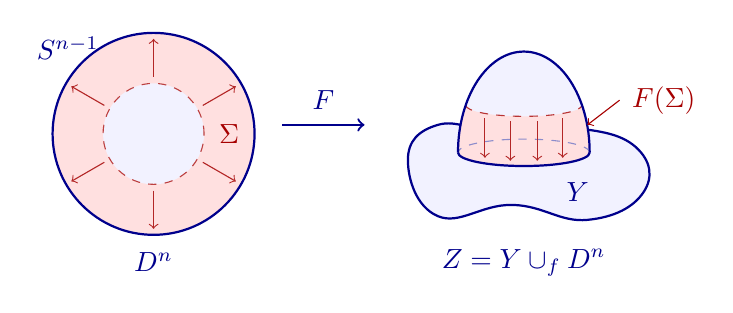
\begin{tikzpicture}[baseline=(current bounding box.center), scale=0.95]
    % === Panel izquierdo: Disco D^n con el collar abierto \Sigma ===
    \begin{scope}
        % Anillo \Sigma y disco interior D^n - \Sigma
        \fill[red!12] (0, 0) circle (1.35);
        \fill[blue!5] (0, 0) circle (0.675);

        % Frontera interior \|x\| = 1/2 (punteada por ser \Sigma abierto) y exterior S^{n-1}
        \draw[dashed, red!65!black!75] (0, 0) circle (0.675);
        \draw[thick, blue!55!black] (0, 0) circle (1.35);

        % Retracción radial por deformación de \Sigma sobre S^{n-1}
        \foreach \ang in {30, 90, 150, 210, 270, 330}{
            \draw[->, thin, red!65!black!85] (\ang:0.76) -- (\ang:1.27);
        }

        % Etiquetas
        \node[red!65!black] at (1.01, 0) {$\Sigma$};
        \node[blue!55!black] at (135:1.62) {$S^{n-1}$};
        \node[blue!55!black] at (0, -1.72) {$D^n$};
    \end{scope}

    % === Flecha F entre ambos espacios ===
    \draw[->, thick, blue!55!black] (1.72, 0.12) -- (2.82, 0.12)
        node[midway, above=2pt] {$F$};

    % === Panel derecho: Espacio adjunto Z = Y \cup_f D^n con F(\Sigma) ===
    \begin{scope}[xshift=4.95cm]
        % Subespacio base Y (región orgánica)
        \filldraw[thick, blue!55!black, fill=blue!5]
            plot[smooth cycle, tension=0.75] coordinates {
                (-1.55, -0.35) (-1.15, 0.12) (-0.30, 0.02)
                ( 0.65,  0.08) ( 1.50,-0.18) ( 1.60,-0.78)
                ( 0.85, -1.15) (-0.15,-0.95) (-1.15,-1.10)
            };

        % Relleno de la celda adjunta F(D^n)
        \fill[blue!5]
            (-0.88, -0.25)
            arc[start angle=180, end angle=360, x radius=0.88, y radius=0.18]
            arc[start angle=0, end angle=180, x radius=0.88, y radius=1.35]
            -- cycle;

        % Relleno del collar F(\Sigma) alrededor de la base de la celda
        \fill[red!12]
            (-0.88, -0.25)
            arc[start angle=180, end angle=360, x radius=0.88, y radius=0.18]
            arc[start angle=0, end angle=28, x radius=0.88, y radius=1.35]
            arc[start angle=360, end angle=180, x radius=0.777, y radius=0.15]
            arc[start angle=152, end angle=180, x radius=0.88, y radius=1.35]
            -- cycle;

        % Arcos posteriores punteados y borde superior abierto de F(\Sigma)
        \draw[dashed, blue!55!black!45]
            (0.88, -0.25) arc[start angle=0, end angle=180, x radius=0.88, y radius=0.18];
        \draw[dashed, red!65!black!80]
            (-0.777, 0.384) arc[start angle=180, end angle=360, x radius=0.777, y radius=0.15];

        % Contorno de la celda y curva de pegado sobre Y
        \draw[thick, blue!55!black]
            (0.88, -0.25) arc[start angle=0, end angle=180, x radius=0.88, y radius=1.35];
        \draw[thick, blue!55!black]
            (-0.88, -0.25) arc[start angle=180, end angle=360, x radius=0.88, y radius=0.18];

        % Retracción por deformación de Y \cup F(\Sigma) sobre Y
        \draw[->, thin, red!65!black!85] (-0.52, 0.21) -- (-0.52, -0.32);
        \draw[->, thin, red!65!black!85] (-0.18, 0.17) -- (-0.18, -0.36);
        \draw[->, thin, red!65!black!85] ( 0.18, 0.17) -- ( 0.18, -0.36);
        \draw[->, thin, red!65!black!85] ( 0.52, 0.21) -- ( 0.52, -0.32);

        % Etiquetas
        \draw[->, thin, red!65!black] (1.28, 0.45) -- (0.85, 0.12);
        \node[red!65!black, right=1pt] at (1.28, 0.45) {$F(\Sigma)$};
        \node[blue!55!black] at (0.72, -0.78) {$Y$};
        \node[blue!55!black] at (0, -1.72) {$Z = Y \cup_f D^n$};
    \end{scope}
\end{tikzpicture}
\]

Consideremos el siguiente diagrama conmutativo inducido por las inclusiones $i, j, k, l$ y por $F$:
\[
{\small
\begin{tikzcd}[column sep=2.2em, row sep=2.8em]
H_q(D^n, S^{n-1}; R)
    \arrow[r, "i_*", "\cong"']
    \arrow[d, "F_*"']
    \arrow[dr, phantom, "\text{(1)}"]
& H_q(D^n, \Sigma; R)
    \arrow[d, "F_*"]
    \arrow[dr, phantom, "\text{(2)}"]
& H_q(D^n - S^{n-1}, \Sigma - S^{n-1}; R)
    \arrow[l, "k_*"', "\cong"]
    \arrow[d, "(F|_{D^n - S^{n-1}})_*", "\cong"'] \\
H_q(Z, Y; R)
    \arrow[r, "j_*", "\cong"']
& H_q(Z, Y \cup F(\Sigma); R)
& H_q(Z - Y, F(\Sigma - S^{n-1}); R)
    \arrow[l, "l_*"', "\cong"]
\end{tikzcd}}
\]

\smallskip
\noindent\textit{Paso 1.} Para ver que $i_*$ es un isomorfismo, consideremos el morfismo entre las sucesiones exactas largas de las parejas $(D^n, S^{n-1})$ y $(D^n, \Sigma)$ inducido por la inclusión $\iota \colon S^{n-1} \hookrightarrow \Sigma$:
\[
{\small
\begin{tikzcd}[column sep=1.45em, row sep=2.4em]
H_q(S^{n-1}; R)
    \arrow[r]
    \arrow[d, "\iota_*", "\cong"']
& H_q(D^n; R)
    \arrow[r]
    \arrow[d, "\operatorname{Id}", "\cong"']
& H_q(D^n, S^{n-1}; R)
    \arrow[r, "\hat{\partial}_q"]
    \arrow[d, "i_*"]
& H_{q-1}(S^{n-1}; R)
    \arrow[r]
    \arrow[d, "\iota_*", "\cong"']
& H_{q-1}(D^n; R)
    \arrow[d, "\operatorname{Id}", "\cong"'] \\
H_q(\Sigma; R)
    \arrow[r]
& H_q(D^n; R)
    \arrow[r]
& H_q(D^n, \Sigma; R)
    \arrow[r, "\hat{\partial}_q"']
& H_{q-1}(\Sigma; R)
    \arrow[r]
& H_{q-1}(D^n; R)
\end{tikzcd}}
\]
Como $S^{n-1}$ es un retracto por deformación radial de $\Sigma$, los homomorfismos $\iota_*$ son isomorfismos. Por el lema del $5$ (\textit{Five Lemma}), resulta que $i_*$ es un isomorfismo.

Para ver que $j_*$ es un isomorfismo aplicamos exactamente el mismo procedimiento: la retracción por deformación radial de $\Sigma$ sobre $S^{n-1}$ deja fijo a $S^{n-1}$ punto a punto, por lo que desciende al cociente y muestra que $Y$ es un retracto por deformación de $Y \cup F(\Sigma)$. Por el lema del $5$, obtenemos que $j_*$ es un isomorfismo.

\smallskip
\noindent\textit{Paso 2.} Analicemos ahora el cuadrado~(2):
\begin{itemize}
    \item La inclusión $k \colon (D^n - S^{n-1}, \Sigma - S^{n-1}) \hookrightarrow (D^n, \Sigma)$ es una escisión por el Teorema de Escisión (con $U = S^{n-1}$ cerrado y $A = \Sigma$ abierto en $D^n$, de modo que $\overline{U} = S^{n-1} \subset \Sigma = \mathring{A}$).
    \item La inclusión $l \colon (Z - Y, F(\Sigma - S^{n-1})) \hookrightarrow (Z, Y \cup F(\Sigma))$ es una escisión por el Teorema de Escisión tomando $U = Y$ y $A = Y \cup F(\Sigma)$ (pues $Y$ es cerrado en $Z$ y $Y \cup F(\Sigma)$ es abierto en $Z$, ya que su preimagen en $Y \sqcup D^n$ es $Y \sqcup \Sigma$, por lo que $\overline{Y} = Y \subset (Y \cup F(\Sigma))^\circ$).
\end{itemize}
En consecuencia, tanto $k_*$ como $l_*$ son isomorfismos. Además, por un ejercicio anterior, $F|_{D^n - S^{n-1}}$ es un homeomorfismo sobre su imagen $Z - Y$ (un encaje abierto), por lo que induce un homeomorfismo de parejas
\[
F|_{D^n - S^{n-1}} \colon (D^n - S^{n-1}, \Sigma - S^{n-1}) \xrightarrow{\;\cong\;} (Z - Y, F(\Sigma - S^{n-1})),
\]
y así $(F|_{D^n - S^{n-1}})_*$ es un isomorfismo.

Finalmente, por la conmutatividad del cuadrado~(2), el homomorfismo vertical central 
$$F_* \colon H_q(D^n, \Sigma; R) \to H_q(Z, Y \cup F(\Sigma); R)$$ es un isomorfismo; y por la conmutatividad del cuadrado~(1), concluimos que $F_* \colon H_q(D^n, S^{n-1}; R) \to H_q(Z, Y; R)$ es un isomorfismo para todo $q$.
\end{dem}
\begin{teorema}[Teorema de los tres incisos]
Sea $f \colon S^{n-1} \to Y$ una función continua ($n \geq 1$) y sea $Z = Y \cup_f D^n$. Denotando por $i \colon Y \hookrightarrow Z$ a la inclusión y por $f_* \colon \widetilde{H}_{n-1}(S^{n-1}; R) \to \widetilde{H}_{n-1}(Y; R)$ al homomorfismo inducido, se cumple:
\begin{enumerate}
    \item $\widetilde{H}_q(Z; R) \cong \widetilde{H}_q(Y; R)$ para todo $q \neq n, n - 1$.
    \item $\widetilde{H}_{n-1}(Z; R) \cong \widetilde{H}_{n-1}(Y; R) / \operatorname{Im} f_*$.
    \item Se tiene una sucesión exacta corta:
    \[
    \begin{tikzcd}[column sep=2.4em]
    0 \arrow[r] & \widetilde{H}_n(Y; R) \arrow[r, "i_*"] & \widetilde{H}_n(Z; R) \arrow[r] & \ker f_* \arrow[r] & 0.
    \end{tikzcd}
    \]
\end{enumerate}
\end{teorema}

\begin{nota}
Si $R$ es un dominio de ideales principales (d.i.p.), por ejemplo un campo o $\mathbb{Z}$, entonces
\[
\widetilde{H}_n(Z; R) \cong \widetilde{H}_n(Y; R) \oplus \ker f_*.
\]
\end{nota}

\begin{dem}
Consideremos la sucesión exacta larga en homología reducida de la pareja $(Z, Y)$, junto con los isomorfismos $F_*$ (de la proposición anterior) y $\hat{\partial}_q$ (de la pareja $(D^n, S^{n-1})$):
\[
{\small
\begin{tikzcd}[column sep=1.9em, row sep=2.2em]
\cdots \arrow[r]
& \widetilde{H}_q(Y; R) \arrow[r, "i_*"]
& \widetilde{H}_q(Z; R) \arrow[r]
& H_q(Z, Y; R) \arrow[r, "\hat{\partial}_q"]
& \widetilde{H}_{q-1}(Y; R) \arrow[r]
& \cdots \\
& & & H_q(D^n, S^{n-1}; R)
    \arrow[u, "F_*", "\cong"']
    \arrow[d, "\hat{\partial}_q", "\cong"']
& & \\
& & & \widetilde{H}_{q-1}(S^{n-1}; R)
    \arrow[uur, "f_*"']
& &
\end{tikzcd}}
\]

Para ver que el triángulo derecho conmuta, consideremos el siguiente diagrama:
\[
\begin{tikzcd}[column sep=3.4em, row sep=2.6em]
H_q(D^n, S^{n-1}; R)
    \arrow[r, "\hat{\partial}_q", "\cong"']
    \arrow[d, "F_*"', "\cong"]
& \widetilde{H}_{q-1}(S^{n-1}; R)
    \arrow[d, "f_*"] \\
H_q(Z, Y; R)
    \arrow[r, "\hat{\partial}_q"']
& \widetilde{H}_{q-1}(Y; R)
\end{tikzcd}
\]
Si colocamos $(F|_{S^{n-1}})_*$ en la flecha vertical derecha (inducido por $F|_{S^{n-1}} \colon S^{n-1} \to Y$), el cuadrado conmuta pues $\hat{\partial}_q$ es una transformación natural. Pero $F|_{S^{n-1}} = f$, ya que para todo $x \in S^{n-1}$ se tiene $F(x) = [x] = [f(x)]$ en $Z = Y \cup_f D^n$; en consecuencia, el cuadrado anterior (y por tanto el triángulo) conmuta.

Sustituyendo cada término $H_q(Z, Y; R)$ por $\widetilde{H}_{q-1}(S^{n-1}; R)$ mediante el isomorfismo $\hat{\partial}_q \circ F_*^{-1}$ (y denotando por $\varphi$ a la composición correspondiente), la sucesión de la pareja $(Z, Y)$ toma la forma
\[
{\small
\begin{tikzcd}[column sep=1.55em]
\cdots \arrow[r]
& \widetilde{H}_q(S^{n-1}; R) \arrow[r, "f_*"]
& \widetilde{H}_q(Y; R) \arrow[r, "i_*"]
& \widetilde{H}_q(Z; R) \arrow[r, "\varphi"]
& \widetilde{H}_{q-1}(S^{n-1}; R) \arrow[r, "f_*"]
& \widetilde{H}_{q-1}(Y; R) \arrow[r]
& \cdots
\end{tikzcd}}
\]
que resulta ser exacta.
%%%% Clase 42 del 16/11/26 inciada el 24/11/26 terminada el 25/11/2026

%%%%%% Clase 43 del 18/11/2026 iniciada el 25/11/2026

Analizamos ahora cada uno de los tres incisos a partir de esta sucesión exacta:
\begin{enumerate}
    \item Si $q \neq n, n - 1$, entonces tanto $\widetilde{H}_q(S^{n-1}; R)$ como $\widetilde{H}_{q-1}(S^{n-1}; R)$ se anulan:
    \[
    {\small
    \begin{tikzcd}[column sep=1.35em, row sep=1.0em]
    \widetilde{H}_q(S^{n-1}; R)
        \arrow[r, "f_*"]
        \arrow[d, phantom, "\cong"{description, sloped, inner sep=1pt}]
    & \widetilde{H}_q(Y; R)
        \arrow[r, "i_*", "\cong"']
    & \widetilde{H}_q(Z; R)
        \arrow[r, "\varphi"]
    & \widetilde{H}_{q-1}(S^{n-1}; R)
        \arrow[r, "f_*"]
        \arrow[d, phantom, "\cong"{description, sloped, inner sep=1pt}]
    & \widetilde{H}_{q-1}(Y; R) \arrow[r]
    & \cdots \\
    0 & & & 0 & &
    \end{tikzcd}}
    \]
    Por exactitud, $i_*$ es un isomorfismo.

    \item Para $q = n - 1$, consideremos el tramo
    \[
    {\small
    \begin{tikzcd}[column sep=1.35em, row sep=1.0em]
    \cdots \arrow[r]
    & \widetilde{H}_n(Z; R) \arrow[r]
    & \widetilde{H}_{n-1}(S^{n-1}; R) \arrow[r, "f_*"]
    & \widetilde{H}_{n-1}(Y; R) \arrow[r, two heads, "i_*"]
    & \widetilde{H}_{n-1}(Z; R) \arrow[r]
    & \widetilde{H}_{n-2}(S^{n-1}; R)
        \arrow[d, phantom, "\cong"{description, sloped, inner sep=1pt}] \\
    & & & & & 0
    \end{tikzcd}}
    \]
    Como $\widetilde{H}_{n-2}(S^{n-1}; R) \cong 0$, el homomorfismo $i_*$ es suprayectivo; aplicando el primer teorema de isomorfismo y la exactitud ($\ker i_* = \operatorname{Im} f_*$), obtenemos
    \[
    \widetilde{H}_{n-1}(Z; R) \cong \widetilde{H}_{n-1}(Y; R) / \ker i_* = \widetilde{H}_{n-1}(Y; R) / \operatorname{Im} f_*.
    \]

    \item Para $q = n$, consideremos el tramo
    \[
    {\small
    \begin{tikzcd}[column sep=1.35em, row sep=1.0em]
    \cdots \arrow[r]
    & \widetilde{H}_n(S^{n-1}; R)
        \arrow[r]
        \arrow[d, phantom, "\cong"{description, sloped, inner sep=1pt}]
    & \widetilde{H}_n(Y; R) \arrow[r, "i_*"]
    & \widetilde{H}_n(Z; R) \arrow[r, "\varphi"]
    & \widetilde{H}_{n-1}(S^{n-1}; R) \arrow[r, "f_*"]
    & \widetilde{H}_{n-1}(Y; R) \\
    & 0 & & & &
    \end{tikzcd}}
    \]
    Como $\widetilde{H}_n(S^{n-1}; R) \cong 0$, el homomorfismo $i_*$ es inyectivo y, por exactitud, $\operatorname{Im}\varphi = \ker f_*$. En consecuencia, la sucesión
    \[
    \begin{tikzcd}[column sep=2.4em, row sep=1.0em]
    0 \arrow[r]
    & \widetilde{H}_n(Y; R) \arrow[r, "i_*"]
    & \widetilde{H}_n(Z; R) \arrow[r, two heads, "\varphi"]
    & \operatorname{Im}\varphi \arrow[r]
        \arrow[d, phantom, "="{description, sloped, inner sep=1pt}]
    & 0 \\
    & & & \ker f_* &
    \end{tikzcd}
    \]
    es exacta.
\end{enumerate}
\end{dem}

\begin{prop}
Para todo $n \geq 0$ se tiene
\[
H_q(\mathbb{C}P^n; R) \cong
\begin{cases}
0 & \text{si } q > 2n \text{ o } q \text{ es impar}, \\
R & \text{si } q \text{ es par y } 0 \leq q \leq 2n.
\end{cases}
\]
\end{prop}

\begin{dem}
Procedemos por inducción sobre $n$. Para el caso base $n = 0$, tenemos $\mathbb{C}P^0 = \{x\}$, de modo que
\[
H_q(\mathbb{C}P^0; R) \cong
\begin{cases}
R & \text{si } q = 0, \\
0 & \text{si } q \neq 0.
\end{cases}
\]

Supongamos ahora que $n \geq 1$ y que conocemos la homología de $\mathbb{C}P^{n-1}$. Por un resultado anterior,
\[
\mathbb{C}P^n \cong \mathbb{C}P^{n-1} \cup_f D^{2n},
\]
donde $f \colon S^{2n-1} \twoheadrightarrow \mathbb{C}P^{n-1}$ es la proyección al cociente. Notemos primero que, por hipótesis de inducción, el homomorfismo
\[
f_* \colon \widetilde{H}_{2n-1}(S^{2n-1}; R) \longrightarrow \widetilde{H}_{2n-1}(\mathbb{C}P^{n-1}; R) \cong 0
\]
es necesariamente nulo ($f_* = 0$), por lo que $\operatorname{Im} f_* = 0$ y $\ker f_* = \widetilde{H}_{2n-1}(S^{2n-1}; R) \cong R$.

Aplicando el Teorema de los tres incisos obtenemos:
\begin{enumerate}
    \item $\widetilde{H}_q(\mathbb{C}P^n; R) \cong \widetilde{H}_q(\mathbb{C}P^{n-1}; R)$ para todo $q \neq 2n, 2n - 1$.
    \item $\widetilde{H}_{2n-1}(\mathbb{C}P^n; R) \cong \widetilde{H}_{2n-1}(\mathbb{C}P^{n-1}; R) / \operatorname{Im} f_* \cong 0$.
    \item Se tiene la sucesión exacta corta
    \[
    \begin{tikzcd}[column sep=2.6em, row sep=1.0em]
    0 \arrow[r]
    & \widetilde{H}_{2n}(\mathbb{C}P^{n-1}; R)
        \arrow[r]
        \arrow[d, phantom, "\cong"{description, sloped, inner sep=1pt}]
    & \widetilde{H}_{2n}(\mathbb{C}P^n; R)
        \arrow[r, "\cong"]
    & \ker f_*
        \arrow[r]
        \arrow[d, phantom, "\cong"{description, sloped, inner sep=1pt}]
    & 0 \\
    & 0 & & R &
    \end{tikzcd}
    \]
    donde $\widetilde{H}_{2n}(\mathbb{C}P^{n-1}; R) \cong 0$ por hipótesis de inducción; luego $\widetilde{H}_{2n}(\mathbb{C}P^n; R) \cong R$.
\end{enumerate}
Dado que $H_q = \widetilde{H}_q$ para $q > 0$ y $H_0(\mathbb{C}P^n; R) \cong \widetilde{H}_0(\mathbb{C}P^n; R) \oplus R \cong R$, se concluye el resultado para $n$.
Por el inciso~1 del Teorema de los tres incisos, tenemos
\[
\widetilde{H}_q(\mathbb{R}P^n; R) \cong \widetilde{H}_q(\mathbb{R}P^{n-1}; R)
\qquad \text{para todo } q \neq n, n - 1.
\]
Para determinar los grados restantes, consideremos la sucesión exacta de la demostración del Teorema de los tres incisos:
\[
{\small
\begin{tikzcd}[column sep=1.9em, row sep=1.0em]
\widetilde{H}_n(S^{n-1}; R) \arrow[r, "f_*"]
& \widetilde{H}_n(\mathbb{R}P^{n-1}; R)
    \arrow[r, "i_*", "\text{(2)}"']
    \arrow[d, phantom, "\cong"{description, sloped, inner sep=1pt}]
& \widetilde{H}_n(\mathbb{R}P^n; R) \arrow[r, hook, "\varphi"]
& \widetilde{H}_{n-1}(S^{n-1}; R) \\
& 0 & & \\[0.8em]
{} \arrow[r, "f_*"]
& \widetilde{H}_{n-1}(\mathbb{R}P^{n-1}; R) \arrow[r, two heads, "i_*", "\text{(1)}"']
& \widetilde{H}_{n-1}(\mathbb{R}P^n; R) \arrow[r]
& \widetilde{H}_{n-2}(S^{n-1}; R)
    \arrow[d, phantom, "\cong"{description, sloped, inner sep=1pt}] \\
& & & 0
\end{tikzcd}}
\]
donde $\widetilde{H}_n(\mathbb{R}P^{n-1}; R) \cong 0$ por hipótesis de inducción (lo cual hace que $\varphi$ sea inyectivo) y $\widetilde{H}_{n-2}(S^{n-1}; R) \cong 0$ (lo cual hace que $i_*$ en (1) sea suprayectivo). Distinguimos dos casos según la paridad de $n$:

\smallskip
\noindent\textit{Caso 1 ($n$ par).} Entonces $n - 1$ es impar y, por la proposición anterior, $f_* \colon \widetilde{H}_{n-1}(S^{n-1}; R) \to \widetilde{H}_{n-1}(\mathbb{R}P^{n-1}; R)$ es multiplicar por $2$. Por (1) y la exactitud ($\ker i_* = \operatorname{Im} f_*$), obtenemos
\[
\widetilde{H}_{n-1}(\mathbb{R}P^n; R)
\overset{\text{(1)}}{\cong}
\frac{\widetilde{H}_{n-1}(\mathbb{R}P^{n-1}; R)}{\ker i_*}
= \frac{\widetilde{H}_{n-1}(\mathbb{R}P^{n-1}; R)}{\operatorname{Im} f_*}
\cong \frac{R}{2R}.
\]
Además, como $\varphi$ es inyectivo con imagen $\ker f_*$, resulta
\[
\widetilde{H}_n(\mathbb{R}P^n; R) \cong \ker f_* \cong R_{(2)}.
\]

\smallskip
\noindent\textit{Caso 2 ($n$ impar).} Entonces $n - 1$ es par y, por la proposición anterior, $f_* = 0$. Usando (2) junto con $\widetilde{H}_n(\mathbb{R}P^{n-1}; R) \cong 0$, se sigue que
\[
\widetilde{H}_n(\mathbb{R}P^n; R) \cong \ker f_* = \widetilde{H}_{n-1}(S^{n-1}; R) \cong R.
\]
En grado $n - 1$, al anularse $f_*$, la sucesión exacta se reduce a
\[
\begin{tikzcd}[column sep=2.2em, row sep=1.0em]
\widetilde{H}_{n-1}(S^{n-1}; R) \arrow[r, "f_* = 0"]
& \widetilde{H}_{n-1}(\mathbb{R}P^{n-1}; R)
    \arrow[r, "i_*", "\cong"']
    \arrow[d, phantom, "\cong"{description, sloped, inner sep=1pt}]
& \widetilde{H}_{n-1}(\mathbb{R}P^n; R) \arrow[r]
& \widetilde{H}_{n-2}(S^{n-1}; R)
    \arrow[d, phantom, "\cong"{description, sloped, inner sep=1pt}] \\
& R_{(2)} & & 0
\end{tikzcd}
\]
donde $\widetilde{H}_{n-1}(\mathbb{R}P^{n-1}; R) \cong R_{(2)}$ por hipótesis de inducción (para $n \geq 3$; si $n = 1$, $\widetilde{H}_0(\mathbb{R}P^0; R) = 0$). En consecuencia, $\widetilde{H}_{n-1}(\mathbb{R}P^n; R) \cong R_{(2)}$.
\end{dem}

\begin{ejemplo}[Construcción de un generador específico para $H_1(S^1; R)$]

Consideremos primero la pareja $(I, \partial I)$, donde $\partial I = \{a, b\}$ (con $a = 0$ y $b = 1$), y su sucesión exacta larga en homología reducida:
\[
{\small
\begin{tikzcd}[column sep=1.5em, row sep=1.0em]
\cdots \arrow[r]
& \widetilde{H}_1(\partial I; R) \arrow[r]
& \widetilde{H}_1(I; R)
    \arrow[r]
    \arrow[d, phantom, "\cong"{description, sloped, inner sep=1pt}]
& H_1(I, \partial I; R) \arrow[r, "\hat{\partial}_1", "\cong"']
& \widetilde{H}_0(\partial I; R) \arrow[r]
& \widetilde{H}_0(I; R)
    \arrow[d, phantom, "\cong"{description, sloped, inner sep=1pt}] \\
& & 0 & & & 0
\end{tikzcd}}
\]
Como $I$ es contraíble, $\widetilde{H}_1(I; R) \cong 0$ y $\widetilde{H}_0(I; R) \cong 0$, por lo que $\hat{\partial}_1 \colon H_1(I, \partial I; R) \xrightarrow{\;\cong\;} \widetilde{H}_0(\partial I; R)$ es un isomorfismo.

Por un resultado anterior (sobre $S^0 = \{a, b\}$), sabemos que
\[
\widetilde{H}_0(\partial I; R) = \{\alpha a + \beta b \mid \alpha + \beta = 0\} \cong R,
\]
mediante el isomorfismo $\alpha a + \beta b \mapsto \alpha$. Tomando el $1$-ciclo relativo $[\operatorname{Id}_I] \in H_1(I, \partial I; R)$, al aplicar $\hat{\partial}_1$ obtenemos
\[
\hat{\partial}_1([\operatorname{Id}_I]) = [b - a] \longmapsto -1 \in R.
\]
Como $-1$ es un generador de $R$ y $\hat{\partial}_1$ es un isomorfismo, concluimos que $[\operatorname{Id}_I]$ es un generador de $H_1(I, \partial I; R)$.

Ahora trasladamos este generador a $S^1$. Consideremos la función continua de parejas $\beta \colon (I, \partial I) \to (S^1, \{1\})$ definida por
\[
\beta(t) = e^{2\pi i t}.
\]
Dado que $\beta$ colapsa toda la frontera $\partial I$ al punto base $1 \in S^1$, se factoriza a través de la proyección cociente $q$ en el triángulo conmutativo
\[
\begin{tikzcd}[column sep=3.4em, row sep=2.8em]
(I, \partial I)
    \arrow[r, "\beta"]
    \arrow[d, "q"']
& (S^1, \{1\}) \\
\left(\dfrac{I}{\partial I}, \{*\}\right)
    \arrow[ur, dashed, "\bar{\beta}"', "\cong"]
&
\end{tikzcd}
\]
donde la función inducida $\bar{\beta}$ es un homeomorfismo de parejas.

Además, tomando $Y = \{y_0\}$ y la función constante $f \colon \partial I \to Y = \{y_0\}$, tenemos la identificación
\[
\left(\frac{I}{\partial I}, \{*\}\right) \cong \bigl(\{y_0\} \cup_f I, \{y_0\}\bigr),
\]
de modo que $q$ corresponde exactamente a la función característica $F \colon (D^1, S^0) \to (Z, Y)$ obtenida al adjuntar una $1$-celda al punto $Y = \{y_0\}$.

Aplicando homología en grado $1$ al triángulo anterior, obtenemos el diagrama conmutativo
\[
\begin{tikzcd}[column sep=3.4em, row sep=2.8em]
H_1(I, \partial I; R)
    \arrow[r, "\beta_*"]
    \arrow[d, "q_*"', "\cong"]
& H_1(S^1, \{1\}; R) \\
H_1\!\left(\dfrac{I}{\partial I}, \{*\}; R\right)
    \arrow[ur, "\bar{\beta}_*"', "\cong"]
&
\end{tikzcd}
\]
Por la proposición anterior sobre adjunción de celdas (aplicada a $F = q$), $q_*$ es un isomorfismo; y como $\bar{\beta}$ es un homeomorfismo, $\bar{\beta}_*$ también lo es. Por lo tanto, $\beta_* = \bar{\beta}_* \circ q_*$ es un isomorfismo.

Finalmente, como $[\operatorname{Id}_I]$ es un generador de $H_1(I, \partial I; R)$, su imagen
\[
\beta_*([\operatorname{Id}_I]) = [\beta]
\]
es un generador de $H_1(S^1, \{1\}; R) = \widetilde{H}_1(S^1; R) = H_1(S^1; R)$.
\end{ejemplo}
\begin{nota}
Si en vez de $\beta$ tomamos una función continua suprayectiva $g \colon I \to S^1$ tal que solamente identifique al $0$ y al $1$, entonces $[g] \in H_1(S^1; R)$ es un generador.
\end{nota}

\begin{lema}[Lema 1]
Consideremos $\Delta^1$ y sea $e_0 = t_0 < t_1 < \dots < t_n = e_1$ una subdivisión de $\Delta^1$. Sea $c \in S_1(\Delta^1)$ la $1$-cadena afín definida por
\[
c = \langle\!\langle t_0, t_1 \rangle\!\rangle + \dots + \langle\!\langle t_{n-1}, t_n \rangle\!\rangle \equiv \sigma_1 + \dots + \sigma_n,
\]
donde cada $\sigma_i = \langle\!\langle t_{i-1}, t_i \rangle\!\rangle \colon \Delta^1 \to \Delta^1$ es un $1$-simplejo afín.
\[
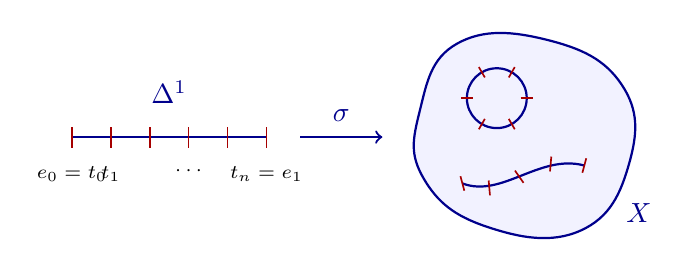
\begin{tikzpicture}[baseline=(current bounding box.center), scale=0.95]
    % === Subdivisión de \Delta^1 ===
    \draw[thick, blue!55!black] (0, 0) -- (2.6, 0);
    \foreach \x in {0, 0.52, 1.04, 1.56, 2.08, 2.60}{
        \draw[semithick, red!65!black] (\x, -0.14) -- (\x, 0.14);
    }
    \node[blue!55!black, above=6pt] at (1.30, 0.10) {$\Delta^1$};
    \node[below=5pt] at (0.00, -0.08) {\scriptsize $e_0 = t_0$};
    \node[below=5pt] at (0.52, -0.08) {\scriptsize $t_1$};
    \node[below=5pt] at (1.56, -0.08) {\scriptsize $\cdots$};
    \node[below=5pt] at (2.60, -0.08) {\scriptsize $t_n = e_1$};

    % === Flecha \sigma ===
    \draw[->, thick, blue!55!black] (3.05, 0) -- (4.15, 0)
        node[midway, above=2pt] {$\sigma$};

    % === Espacio X con imagen subdividida (curva abierta y lazo) ===
    \begin{scope}[xshift=6.0cm]
        \filldraw[thick, blue!55!black, fill=blue!5]
            plot[smooth cycle, tension=0.75] coordinates {
                (-1.35,  0.35) (-0.85,  1.25) ( 0.35,  1.30)
                ( 1.35,  0.70) ( 1.45, -0.35) ( 0.80, -1.25)
                (-0.45, -1.20) (-1.30, -0.55)
            };

        % Caso cerrado: \sigma(e_0) = \sigma(e_1)
        \draw[thick, blue!55!black] (-0.32, 0.52) circle (0.40);
        \foreach \ang in {0, 60, 120, 180, 240, 300}{
            \draw[semithick, red!65!black]
                (-0.32, 0.52) ++(\ang:0.32) -- ++(\ang:0.16);
        }

        % Caso general: trayectoria subdividida
        \draw[thick, blue!55!black]
            (-0.78, -0.62) .. controls (-0.25, -0.82) and (0.25, -0.22) .. (0.85, -0.38);
        \foreach \px/\py/\ang in {
            -0.78/-0.62/105,
            -0.42/-0.68/95,
            -0.02/-0.53/125,
             0.40/-0.36/85,
             0.85/-0.38/75
        }{
            \draw[semithick, red!65!black]
                (\px, \py) ++(\ang:-0.10) -- ++(\ang:0.20);
        }

        \node[blue!55!black] at (1.58, -1.02) {$X$};
    \end{scope}
\end{tikzpicture}
\]
Sea $\sigma \colon \Delta^1 \to X$ un $1$-simplejo singular. Entonces
\[
\sigma - \sigma_\#(c) \in B_1(X),
\]
y por lo tanto $[\sigma - \sigma_\#(c)] = 0 \in H_1(X; R)$. En particular, si $\sigma(e_0) = \sigma(e_1)$, se tiene que
\[
[\sigma] = [\sigma_\#(c)] \in H_1(X; R).
\]
\end{lema}

\begin{dem}
Consideremos $\operatorname{Id}_{\Delta^1} \colon \Delta^1 \to \Delta^1$ en $S_1(\Delta^1)$, cuya frontera es $\partial_1(\operatorname{Id}_{\Delta^1}) = e_1 - e_0$. Por otro lado, para la $1$-cadena $c$ tenemos
\begin{align*}
\partial_1(c) &= (t_1 - t_0) + (t_2 - t_1) + \dots + (t_n - t_{n-1}) \\
&= t_n - t_0 = e_1 - e_0.
\end{align*}
Por lo tanto, $\partial_1(\operatorname{Id}_{\Delta^1} - c) = 0$, es decir, $\operatorname{Id}_{\Delta^1} - c$ es un $1$-ciclo en $\Delta^1$. Como $\Delta^1$ es contraíble, se cumple $H_1(\Delta^1; R) \cong 0$, de modo que existe $d \in S_2(\Delta^1)$ tal que $\partial_2(d) = \operatorname{Id}_{\Delta^1} - c$.

Aplicando el morfismo de cadenas $\sigma_\#$, obtenemos
\begin{align*}
\sigma - \sigma_\#(c) &= \sigma_\#(\operatorname{Id}_{\Delta^1}) - \sigma_\#(c) \\
&= \sigma_\#(\operatorname{Id}_{\Delta^1} - c) \\
&= \sigma_\#(\partial_2(d)) \\
&= \partial_2(\sigma_\#(d)) \in B_1(X).
\end{align*}
En particular, si $\sigma(e_0) = \sigma(e_1)$, tanto $\sigma$ como $\sigma_\#(c)$ son ciclos y sus clases coinciden: $[\sigma] = [\sigma_\#(c)]$.
\end{dem}

\begin{lema}[Lema 2]
Sea $\iota \colon \Delta^1 \to \Delta^1$ una función continua tal que $\iota(e_0) = e_1$ y $\iota(e_1) = e_0$, y sea $\sigma \colon \Delta^1 \to X$ una función continua. Entonces
\[
\sigma + \sigma_\#(\iota) \in B_1(X).
\]
En particular, si $\sigma(e_0) = \sigma(e_1)$, entonces
\[
[\sigma_\#(\iota)] = [\sigma \circ \iota] = -[\sigma] \in H_1(X; R).
\]
\end{lema}

\begin{dem}
Consideremos $\iota$ y $\operatorname{Id}_{\Delta^1}$ en $S_1(\Delta^1)$. Sus fronteras son
\[
\partial_1(\iota) = e_0 - e_1
\qquad \text{y} \qquad
\partial_1(\operatorname{Id}_{\Delta^1}) = e_1 - e_0,
\]
por lo que $\partial_1(\operatorname{Id}_{\Delta^1} + \iota) = 0$. En consecuencia, $[\operatorname{Id}_{\Delta^1} + \iota] \in H_1(\Delta^1; R) \cong 0$, así que existe $b \in S_2(\Delta^1)$ tal que $\partial_2(b) = \operatorname{Id}_{\Delta^1} + \iota$.

Aplicando $\sigma_\#$, resulta
\begin{align*}
\sigma + \sigma_\#(\iota) &= \sigma_\#(\operatorname{Id}_{\Delta^1}) + \sigma_\#(\iota) \\
&= \sigma_\#(\operatorname{Id}_{\Delta^1} + \iota) \\
&= \sigma_\#(\partial_2(b)) \\
&= \partial_2(\sigma_\#(b)) \in B_1(X).
\end{align*}
Si $\sigma$ es un ciclo (es decir, $\sigma(e_0) = \sigma(e_1)$), esto implica $[\sigma_\#(\iota)] = -[\sigma] \in H_1(X; R)$. (Un ejemplo explícito de tal función $\iota \colon \Delta^1 = I \to \Delta^1 = I$ es $\iota(t) = 1 - t$.)
\end{dem}

\medskip
Recordemos que para calcular la homología relativa $H_*(X, A; R)$ definimos el complejo de cadenas relativas como
\[
S_*(X, A) = \frac{S_*(X)}{S_*(A)},
\]
obteniendo la sucesión exacta corta de complejos de cadenas
\[
\begin{tikzcd}[column sep=2.4em]
0 \arrow[r] & S_*(A) \arrow[r] & S_*(X) \arrow[r] & S_*(X, A) \arrow[r] & 0,
\end{tikzcd}
\]
la cual induce la sucesión exacta larga en homología:
\[
\begin{tikzcd}[column sep=2.2em]
\cdots \arrow[r] & H_q(A; R) \arrow[r] & H_q(X; R) \arrow[r] & H_q(X, A; R) \arrow[r] & H_{q-1}(A; R) \arrow[r] & \cdots
\end{tikzcd}
\]

%%%% Clase 43 del 18/11/26 inciada el 25/11/26 terminada el 25/11/2026

%%%%%% Clase 44 del 20/11/2026 iniciada el 25/11/2026


